\documentclass[12pt]{article}

\usepackage{KUstyle}
\usepackage[margin=0.8in]{geometry} % Package for pagemargin
\usepackage{setspace} % Package for linespacing
\usepackage{tabularx} % Package for table
\usepackage{fontspec}
\usepackage{enumitem}

\usepackage[utf8]{inputenc}
\usepackage[english]{babel}
\usepackage{csquotes}
\usepackage{xpatch}
\usepackage{blindtext}
\usepackage{url}
\usepackage{tcolorbox}
\usepackage{bbold}
\usepackage{caption}
\usepackage{subcaption}
\usepackage{multirow}

\usepackage[
   backend=biber,
   style=phys,
   articletitle=true,
   biblabel=brackets,
   chaptertitle=false,
   pageranges=false,
   eprint=true,
]{biblatex}
\addbibresource{refs.bib}

\usepackage{amsmath}
\usepackage{amssymb}
\usepackage{amsfonts}
\usepackage{mathtools}
\usepackage{multirow}
\usepackage{hhline}
\usepackage{slashed}
\usepackage{shuffle}
\usepackage{braket}

\usepackage{tikz}
\usetikzlibrary{decorations.pathmorphing}
\usetikzlibrary{decorations.markings}
\usetikzlibrary{arrows}

% This change the content of the frontpage
\ptype{Master's thesis}
\author{Jo Nykrem}
%\title{Generalisations of the Double Copy}
\title{Bootstrapping Tree Amplitudes using Loop Tools}
\subtitle{}
\date{Date: {April 2, 2024}}
\supervisor{Supervisors: {N. Emil J. Bjerrum-Bohr, Zhengwen Liu}}
%\fpimage{picture.png} % Remove this command if no image is desired

\renewcommand{\contentsname}{Table of content}

\newcommand{\del}{\partial}
\newcommand{\vphi}{\varphi}

\renewcommand{\a}[1]{\alpha_{#1}}
\newcommand{\e}[1]{\epsilon_{#1}}
\newcommand{\ee}[2]{(\epsilon_{#1}\epsilon_{#2})}
\newcommand{\pe}[2]{(p_{#1}\epsilon_{#2})}
\newcommand{\ep}[2]{(\epsilon_{#1}p_{#2})}
\newcommand{\pp}[2]{(p_{#1}p_{#2})}

\newcommand{\EE}[4]{(\epsilon_{#1}^{#2}\cdot\epsilon_{#3}^{#4})}
\newcommand{\pE}[3]{(p_{#1}\cdot\epsilon_{#2}^{#3})}

\renewcommand{\d}[2]{{#1}\cdot{#2}}
\newcommand{\comma}{\,,\,}

%\newcommand{\footcomment}[1]{\let\thefootnote\relax\footnote{#1}}

\DeclareMathOperator{\tr}{Tr}

\definecolor{maroonKU}{RGB}{144, 26, 30}
\newcommand{\zl}[1]{[{\color{maroonKU}{ZL}:~{#1}}]}

%\setlength\parindent{0pt}

\begin{document}

\maketitle

\onehalfspacing

\newpage

\begin{abstract}
% The thesis desires to study extensions and potential
% obstructions of double-copy structures at the tree level. In this
% thesis, we want to highlight the implication of double-copy
% relations induced by introducing higher derivative couplings in
% the theories, concentrating on Yang-Mills and Gravity. Such
% higher derivative coupling is required in numerous areas of
% particle physics and is critical for effective field theory
% descriptions. Our analysis uses a bootstrap/first principles
% method to compute gauge invariant amplitude candidates.
% These are interesting in and of themselves and their mapping
% at the Lagrangian level. For higher points, our analysis
% includes loop tools and finite field frameworks demanded at
% tree-level scattering. We will also examine the state of the art
% in the field.
The thesis presents a method of bootstrapping the S-matrix based on a first-principle approach to scattering amplitudes and its symmetries. The focus is on massless gauge bosons, including gluons and gravitons, motivated by the celebrated double copy relation between gauge and gravity theories. We propose a method of utilising computational tools from the field of loop integral calculations to solve large linear systems arising in the bootstrap. We also consider effective couplings and how these can be identified from solutions to the linear systems. 
%We also give a review of the state of the art in the field.
\end{abstract}








\newpage

\tableofcontents

\newpage

\section{Introduction}

%\begin{description}
%    \item[What are scattering amplitudes?] Probability measure
%    \item[Applications] Collider physics, quantum qravity, gravitational waves
%    \item[On-shell methods] Spinor-helicity framework, recursion relations, unitarity   
%\end{description}

%\subsection{[Title 2]}
%\subsection{[Title 2]}


Scattering amplitudes, known also as S-matrix elements, are mathematical objects that describe the probabilities of possible outcomes when elementary particles interact with each other. The importance of scattering amplitudes is profound. They allow physicists to make precise predictions for the outcomes of high-energy particle scattering experiments, such as the Large Hadron Collider (LHC) at CERN. For instance, the discovery of the Higgs boson would not have been possible without a deep understanding of scattering amplitudes. Furthermore, they provide a window into the intricacies of quantum field theory, potentially revealing hidden structures within this framework.

While Feynman diagrams are a common tool for calculating scattering amplitudes in perturbative quantum field theory (as described in standard textbooks), their usefulness has limitations. As the number of external particles or loops in a scattering process increases, the sheer number of diagrams explodes, making calculations cumbersome. Interestingly, despite this complexity, the final answers for scattering amplitudes often turn out to be surprisingly simple. This suggests that Feynman diagrams might be obscuring underlying patterns and cancellations that lead to simple final results.

Driven by this intriguing observation, theoretical physicists have embarked on a quest for alternative methods to understand and compute scattering amplitudes, bypassing Feynman diagrams. The past few decades have witnessed significant breakthroughs in this pursuit, with advancements in on-shell recursion relations, unitarity methods, and the bootstrap technique. Comprehensive reviews on these topics can be found in e.g.\,\cite{Elvang:2015rqa,Cheung:2017pzi}.

The bootstrap method, with roots in the S-matrix program \cite{Eden:1966dnq}, offers a fascinating approach. The core idea is that on-shell scattering amplitudes can potentially be determined by their inherent properties, such as symmetries and analyticity. Recent studies in e.g.\,\cite{Boels:2016xhc, Boels:2017gyc} have demonstrated that on-shell gauge invariance can give strong constraints for amplitudes involving gluons and gravitons. The purpose of this thesis is to further investigate this novel method, with a particular focus on developing efficient techniques to solve the large linear systems that arise in the bootstrap approach for tree-level amplitudes.

This thesis is organized as follows. Chapter \ref{sec:the-s-matrix} provides a foundational review of Poincaré symmetry, particles, and scattering amplitudes. Then, in Chapter \ref{sec:quantum-field-theory}, we briefly review quantum field theory and Feynman diagram formalism. In Chapter \ref{sec:bootstrapping-the-s-matrix}, we discuss the bootstrap method in detail, including its fundamental idea, working framework, and illustrative examples for three and four-particle scattering. This chapter will also highlight a key finding: algorithms and tools initially developed for reducing loop-level amplitudes (Feynman integrals) can be effectively repurposed to reduce linear systems encountered while bootstrapping tree-level amplitudes. We conclude the thesis in Chapter \ref{sec:conclusion-and-outlook}.

\newpage
%\section{Scattering Amplitudes}
\section{The S-matrix}
\label{sec:the-s-matrix}

\subsection{Lorentz symmetry} \label{subsec:ch2-symmetry}
%Following {Boels:2016xhc,

%Following Weinberg vol 1 \cite{Weinberg:1995mt}, section 2.5, give a review about ``particle = irreducible representation of the little group''.

%\begin{tcolorbox}[standard jigsaw, opacityback=0]
%		First introduce the notion of physical states in Hilbert space as we know it from quantum mechanics. This emphasises Unitary transformations and Hermitian operators. Then over to space-time symmetries, in particular Poincaré symmetry. That is: the Lorentz group and the set of space-time translations. 
%\end{tcolorbox}


%We believe the Poincaré group describes  Any physical state must transform according
%
%The Lorentz group is a subgroup of the Poincaré group and is th
%
%To be able to talk about scattering amplitudes we need to clearly understand what we mean by particles scattering off each other. Especially we need to define particles as irreducible representations of the Poincaré group.
%
%The Poincaré group is made up of the group of translations in space time
%
%A physical state must remain invariant under the set of transformations contained in the Poincaré group. Its subgroups are the Lorentz group and the group of space-time translations. The generators of the Lorentz group are given by the 
%
%\begin{equation}
%	x^\mu \rightarrow x^\mu + a^\mu \,,
%\end{equation}
%
%and the Lorentz group. The latter consisting of boosts and rotations contained in the antisymmetric 
%
%Poincaré transformation
%
%\begin{equation}
%	x^\mu \rightarrow \Lambda^{\mu}{}_{\nu}\,x^\nu + a^\mu
%\end{equation}
%
%Lorentz transformation


Any theory of nature that aims to describe reality must obey certain symmetries. That is, a given physical state must remain invariant under certain symmetry transformations. One of the most fundamental symmetries is given by the Poincaré group\footnote{Or the inhomogeneous Lorentz group \cite{Weinberg:1995mt}.}, which is a semi-direct product of its subgroups: the group of translations in $D$-dimensional space-time\footnote{In this chapter we are working in D-dimensional space-time, unless stated otherwise.}, denoted $\mathbb{R}^D$, and the Lorentz group, denoted $\operatorname{SO}(D-1,1)$\footnote{More precisely, the restricted Lorentz group, in which all transformations preserve the orientation of space and time.}. The transformation of a $D$-vector under the Poincaré group, a so-called Poincaré transformation, can be stated as
\begin{equation}
\label{eq:sec2:poincaré-transformation}
	x^\mu \rightarrow {x^{\prime}}^{\mu} = \Lambda^{\mu}{}_{\nu} x^{\nu} + a^{\mu} \,.
\end{equation}
Here, $\Lambda$ is an element of the (restricted)\footnote{Implying $\det\Lambda = 1$ and $\Lambda^{0}{}_{0} \geq 0\,$.} Lorentz group and $a$ is a an element of the translation group. The elements of the Lorentz group are the set of matrices that preserves the space-time interval, meaning ${x^2 \equiv \eta_{\mu\nu} x^\mu x^\nu}$ is the same in all reference frames, with $\eta_{\mu\nu}$ being the metric and $x^{\mu}$ a $D$-vector. Consequentially, the metric will place some restrictions on $\Lambda$. To this end, we set $a = 0$ in \eqref{eq:sec2:poincaré-transformation}, giving the Lorentz transformation,
\begin{equation}
\label{eq:sec2:lorentz-transformation}
	x^{\mu} \rightarrow {x^{\prime}}^{\mu} = \Lambda^{\mu}{}_{\nu}x^{\nu} \,.
\end{equation}
Now, we compare the space-time interval in two different reference frames:
\begin{equation}
\begin{aligned}
	x^2 = \eta_{\mu\nu}x^{\mu}x^{\nu} &= \eta_{\mu\nu}{x^{\prime}}^{\mu}{x^{\prime}}^{\nu} \\
	&= \eta_{\mu\nu}\Lambda^{\mu}{}_{\rho}\Lambda^{\nu}{}_{\sigma}x^{\rho}x^{\sigma} \\
	&= \eta_{\rho\sigma}\Lambda^{\rho}{}_{\mu}\Lambda^{\sigma}{}_{\nu}x^{\mu}x^{\nu} = {x'}^2 \,.
\end{aligned}	
\end{equation}
This implies that the elements of the Lorentz group obeys
\begin{equation}
	\eta_{\mu\nu} = \eta_{\rho\sigma}\Lambda^{\rho}{}_{\mu}\Lambda^{\sigma}{}_{\nu} \,,
\end{equation}
as well as the existence of an inverse element, $(\Lambda^{-1})^{\mu}{}_{\nu} = \Lambda_{\nu}{}^{\mu}$ \cite{Srednicki:2007qs}.
Looking at two consecutive Poincaré transformations, as given by \eqref{eq:sec2:poincaré-transformation}, leads us to the composition rule of the group:
\begin{equation}
\label{eq:sec2:composition-rule}
\begin{aligned}
	{x^{\prime\prime}}^{\mu} &= \tilde{\Lambda}^{\mu}{}_{\nu}{x^{\prime}}^{\nu} + \tilde{a}^{\mu} \\
	&= \tilde{\Lambda}^{\mu}{}_{\nu}(\Lambda^{\nu}{}_{\rho}x^{\rho} + a^{\nu}) + \tilde{a}^{\mu} \\
	&= \tilde{\Lambda}^{\mu}{}_{\nu}\Lambda^{\nu}{}_{\rho}x^{\rho} + \tilde{\Lambda}^{\mu}{}_{\nu}a^{\nu} + \tilde{a}^{\mu} \\
	&= (\tilde{\Lambda}{\Lambda}x)^{\mu} + (\tilde{\Lambda}a + \tilde{a})^{\mu}.
\end{aligned}
\end{equation}
We can expand the Lorentz transformation around the identity by writing
\begin{equation}\label{eq:sec2:lorentz-expansion}
	\Lambda^{\mu}{}_{\nu} = \delta^{\mu}{}_{\nu} + \omega^{\mu}{}_{\nu}
\end{equation}
for some infinitesimal $\omega$. Inserting \eqref{eq:sec2:lorentz-expansion} into \eqref{eq:sec2:composition-rule} leads to
\begin{equation}
\begin{aligned}
	\eta_{\mu\nu} &= \eta_{\rho\sigma}(\delta^{\rho}{}_{\mu} + \omega^{\rho}{}_{\mu})(\delta^{\sigma}{}_{\nu} + \omega^{\sigma}{}_{\nu}) \\
	&= \eta_{\rho\sigma}\delta^{\rho}{}_{\mu}\delta^{\sigma}{}_{\nu} + \eta_{\rho\sigma}\delta^{\rho}{}_{\mu}\omega^{\sigma}{}_{\nu} + \eta_{\rho\sigma}\omega^{\rho}{}_{\mu}\delta^{\sigma}{}_{\nu} + \mathcal{O}(\omega^2) \\
	&= \eta_{\mu\nu} + \eta_{\mu\sigma}\omega^{\sigma}{}_{\nu} + \eta_{\rho\nu}\omega^{\rho}{}_{\mu} + \mathcal{O}(\omega^2) \\
	&= \eta_{\mu\nu} + \omega_{\mu\nu} + \omega_{\nu\mu} + \mathcal{O}(\omega^2) \,.
\end{aligned}	
\end{equation}
Keeping only terms linear in $\omega$ we get 
\begin{equation}\label{}
\omega_{\mu\nu} = -\omega_{\nu\mu} \,.
\end{equation}
We let a general Poincaré transformation take the form $U(\Lambda,a)$ and expand it around the identity $U(\mathbb{1},0)$. This gives us, to leading order, the infinitesimal Poincaré transformation ${U(\mathbb{1}+\omega,\epsilon)}$, where $\epsilon$ is taken to be an infinitesimal translation. Examining how this transforms under a general Poincaré transformation will give us some more insights. Firstly, using \eqref{eq:sec2:composition-rule} and noticing that $U^{-1}(\mathbb{1}+\omega,a) = U(\Lambda^{-1},-\Lambda^{-1}a)$, we get
\begin{equation} \label{eq:ch2-infinitesimal_composition}
	U(\Lambda,a)U(\mathbb{1}+\omega,\epsilon)U^{-1}(\Lambda,a) = U(\mathbb{1}+\Lambda\omega\Lambda^{-1},\Lambda\epsilon-\Lambda\omega\Lambda^{-1}a) \,.
\end{equation}
A result from group theory states that any group action can be expanded infinitesimally using the generators of the group \cite{Zee:2016fuk}. In the case of the Poincaré group these generators are $M_{\mu\nu}$, composed of rotations and boosts, and $P_\mu$, the generator of translations. Therefore we can write the infinitesimal Poincaré transformation as
\begin{equation} \label{eq:ch2-infinitesimal_poincaré_transformation}
	U(\mathbb{1}+\omega,\epsilon) = \mathbb{1} - \frac{i}{2}\omega^{\mu\nu}M_{\mu\nu} + i\epsilon^{\mu}P_{\mu} + \cdots \,.
\end{equation}
Now we compute \eqref{eq:ch2-infinitesimal_composition} using the generators of the group, $M_{\mu\nu}$ and $P_{\mu}$:
\begin{equation} \label{eq:ch2-transformation-generators}
	\begin{aligned}
		&U(\Lambda,a)(\mathbb{1} - \frac{i}{2}\omega^{\mu\nu}M_{\mu\nu} + i\epsilon^{\mu}P_{\mu})U^{-1}(\Lambda,a) \\
		&= \mathbb{1} - \frac{i}{2}(\Lambda\omega\Lambda^{-1})^{\mu\nu}M_{\mu\nu} + i(\Lambda\epsilon - \Lambda\omega\Lambda^{-1}a)^{\mu}P_{\mu} \\
		&= \mathbb{1} - \frac{i}{2}\Lambda^{\mu}{}_{\rho}\omega^{\rho\sigma}(\Lambda^{-1})_{\sigma}{}^{\nu}M_{\mu\nu} + i\Lambda^{\mu}{}_{\nu}\epsilon^{\nu}P_{\mu} - i\Lambda^{\mu}{}_{\rho}\omega^{\rho\sigma}(\Lambda^{-1})_{\sigma}{}^{\nu}a_{\nu}P_{\mu} \\
		&= \mathbb{1} - \frac{i}{2}\omega^{\rho\sigma}\Lambda^{\mu}{}_{\rho}(\Lambda^{-1})_{\sigma}{}^{\nu}(M_{\mu\nu} - 2a_{\nu}P_{\mu}) + i\epsilon^{\nu}\Lambda^{\mu}{}_{\nu}P_{\mu} \\
		&= \mathbb{1} - \frac{i}{2}\omega^{\rho\sigma}\Lambda^{\mu}{}_{\rho}\Lambda^{\nu}{}_{\sigma}(M_{\mu\nu} - a_{\nu}P_{\mu} + a_{\mu}P_{\nu}) + i\epsilon^{\nu}\Lambda^{\mu}{}_{\nu}P_{\mu}
	\end{aligned}
\end{equation}
By comparing the first and last lines of \eqref{eq:ch2-transformation-generators}, we see that the generators transform according to
\begin{align}
	\label{eq:ch2-lorentz_generators_transformation}
	U(\Lambda, a)M_{\mu\nu}U^{-1}(\Lambda, a) &= \Lambda^{\rho}{}_{\mu}\Lambda^{\sigma}{}_{\nu}(M_{\rho\sigma} - a_{\rho}P_{\sigma} + a_{\sigma}P_{\rho}) \\
	\label{eq:ch2-momentum-generator-transformation}
	U(\Lambda, a)P_{\mu}U^{-1}(\Lambda, a) &= \Lambda^{\nu}{}_{\mu}P_{\nu} \,.
\end{align}
Now we make $\Lambda$ and $a$ infinitesimal in \eqref{eq:ch2-lorentz_generators_transformation} by setting $\Lambda^{\mu}{}_{\nu} = \delta^{\mu}{}_{\nu} + \omega^{\mu}{}_{\nu}$ and $a^{\mu} = \epsilon^{\mu}$,
\begin{equation} \label{eq:ch2-lorentz_generators_sandwich_1}
	U(\mathbb{1}+\omega,\epsilon)M_{\mu\nu}U^{-1}(\mathbb{1}+\omega, \epsilon) = (\delta^{\rho}{}_{\mu} + \omega^{\rho}{}_{\mu})(\delta^{\sigma}{}_{\nu} + \omega^{\sigma}{}_{\nu})(M_{\rho\sigma} - \epsilon_{\sigma}P_{\rho} + \epsilon_{\sigma}P_{\rho}) \,.
\end{equation}
This enables us to see how the generators transforms in two ways and deduce from that the commutator relations between the generators, which defines the Lie algebra of the Poincaré group. Using \eqref{eq:ch2-infinitesimal_poincaré_transformation} the generators transforms as
\begin{equation} \label{eq:ch2-lorentz_generators_sandwich_2}
	U(\mathbb{1}+\omega, \epsilon)M_{\mu\nu}U^{-1}(\mathbb{1}+\omega, \epsilon) = (\mathbb{1} + \frac{i}{2}\omega^{\rho\sigma}M_{\rho\sigma} + i\epsilon^{\rho}P_{\rho} + \cdots)M_{\mu\nu}(\mathbb{1} - \frac{i}{2}\omega^{\rho\sigma}M_{\rho\sigma} - i\epsilon^{\rho}P_{\rho} + \cdots) \,.
\end{equation}
Computing \eqref{eq:ch2-lorentz_generators_sandwich_1} we get
\begin{equation} \label{eq:ch2-generators_transformation_1}
	\begin{aligned}
	&(\delta^{\rho}{}_{\mu} + \omega^{\rho}{}_{\mu})(\delta^{\sigma}{}_{\nu} + \omega^{\sigma}{}_{\nu})(M_{\rho\sigma} - \epsilon_{\sigma}P_{\rho} + \epsilon_{\sigma}P_{\rho}) \\
		&= M_{\mu\nu} + \omega^{\sigma}{}_{\nu}M_{\mu\sigma} + \omega^{\rho}{}_{\mu}M_{\rho\nu} - \epsilon_{\mu}P_{\nu} + \epsilon_{\nu}P_{\mu} + \mathcal{O}(\omega^{2},\omega\epsilon) \\
		&= M_{\mu\nu} - \omega^{\rho\sigma}\eta_{\nu\rho}M_{\mu\sigma} - \omega^{\rho\sigma}\eta_{\mu\sigma}M_{\nu\rho} - \epsilon^{\rho}\eta_{\mu\rho}P_{\nu} + \epsilon^{\rho}\eta_{\nu\rho}P_{\mu} + \mathcal{O}(\omega^{2},\omega\epsilon) \\
		&= M_{\mu\nu} - \frac{1}{2}\omega^{\rho\sigma}(\eta_{\nu\rho}M_{\mu\sigma} - \eta_{\nu\sigma}M_{\mu\rho} + \eta_{\mu\sigma}M_{\nu\rho} - \eta_{\mu\rho}M_{\nu\sigma}) - \epsilon^{\rho}(\eta_{\mu\rho}P_{\nu} - \eta_{\nu\rho}P_{\mu}) + \mathcal{O}(\omega^{2},\omega\epsilon) \,. \\
	\end{aligned}
\end{equation}
Next we compute \eqref{eq:ch2-lorentz_generators_sandwich_2}:
\begin{equation} \label{eq:ch2-generators_transformation_2}
	\begin{aligned}
		&U(\mathbb{1}+\omega, \epsilon)M_{\mu\nu}U^{-1}(\mathbb{1}+\omega, \epsilon) \\
		&= (\mathbb{1} + \frac{i}{2}\omega^{\rho\sigma}M_{\rho\sigma} + i\epsilon^{\rho}P_{\rho} + \cdots)M_{\mu\nu}(\mathbb{1} - \frac{i}{2}\omega^{\rho\sigma}M_{\rho\sigma} - i\epsilon^{\rho}P_{\rho} + \cdots) \\
		&= M_{\mu\nu} - \frac{i}{2}\omega^{\rho\sigma}M_{\mu\nu}M_{\rho\sigma} + \frac{i}{2}\omega^{\rho\sigma}M_{\rho\sigma}M_{\mu\nu} - i\epsilon^{\rho}M_{\mu\nu}P_{\rho} + i\epsilon^{\rho}P_{\rho}M_{\mu\nu} + \mathcal{O}(\omega^{2},\epsilon^{2},\omega\epsilon) \\
		&= M_{\mu\nu} - \frac{i}{2}\omega^{\rho\sigma}[M_{\mu\nu},M_{\rho\sigma}] - i\epsilon^{\rho}[M_{\mu\nu},P_{\rho}] + \mathcal{O}(\omega^{2},\epsilon^{2},\omega\epsilon)
	\end{aligned}
\end{equation}
From the last lines in \eqref{eq:ch2-generators_transformation_1} and \eqref{eq:ch2-generators_transformation_2} we get the commutator relations
\begin{align}
\begin{aligned}
		i[M_{\mu\nu},M_{\rho\sigma}] &= \eta_{\nu\rho}M_{\mu\sigma} - \eta_{\nu\sigma}M_{\mu\rho} - \eta_{\mu\rho}M_{\nu\sigma} + \eta_{\mu\sigma}M_{\nu\rho} \,, \\
		i[M_{\mu\nu},P_{\rho}] &=  \eta_{\mu\rho}P_{\nu} - \eta_{\nu\rho}P_{\mu} \,, \\
		[P_{\mu},P_{\nu}] &= 0 \,.
\end{aligned}
\end{align}
Finally, we have derived the Lie algebra of the Poincaré group. The first line describes the algebra of the Lorentz group, i.e. $\operatorname{SO}(D{-}1,1)$.

Now we want to classify particle states as irreducible representations of the Poincaré group. We start with two representative states in $D=4$ that are eigenstates of the generator of translations, with momenta given by:
\begin{equation}
\label{eq:sec2:representative-states}
    \begin{split}
        p_m^\mu &= \{m,0,0,0\} \\
        p_\omega^\mu &= \{\omega,0,0,\omega\}
    \end{split}
\end{equation}
The first line in \eqref{eq:sec2:representative-states} describes a massive particle in its rest frame and the second line describes a massless particle traveling in the $z$-direction. The maximal subgroups of the Lorentz group that leaves the two momentum vectors invariant are $SO(3)$ and $ISO(2)$, respectively. These subgroups are known as little groups. Further, we classify each state according to the irreducible representation of the corresponding little group. For that purpose we introduce the two Casimir invariants,
\begin{equation}
    C_1 = P_{\mu}P^{\mu}
\end{equation}
and
\begin{equation}
    C_2 = W_{\mu}W^{\mu} \,.
\end{equation}
Here, $P^\mu$ is the generator of translations and $W^\mu$ is the Pauli-Lubanski vector given by \cite{Zee:2016fuk}
\begin{equation}
\label{eq:sec2:pauli-lubanski-vector}
    W^\sigma = \frac{1}{2}\epsilon^{\mu\nu\rho\sigma}M_{\mu\nu}P_{\rho} \,.
\end{equation}
The Casimir invariants readily commutes with all the generators of the Poincaré group, therefore their eigenvalues will work as labels for states they act upon. The massive representative state is labeled by its mass, $m$, and spin, $s$. In the massless case the spin label is replaced by the helicity of the particle, $\lambda$, the component of angular momentum in the direction of motion. For a detailed discussion, we refer to Weinberg's book \cite{Weinberg:1995mt}. In this work, we focus only on massless particles.

\subsection{Particles}\label{subsec:ch2-particles}

As we have seen Poincaré symmetry leads to the classification of particles as irreducible representations (irreps) of the little group \cite{Wigner:1939cj}. Specifically, in the $D$-dimensional spacetime, the little groups that characterize physical massless and massive particles are $\operatorname{ISO}(D{-}2)$\footnote{Isometry group (or Euclidean group) of the $(D-2)$-dimensional plane \cite{Schwartz:2014sze}.} and $\operatorname{SO}(D{-}1)$, respectively.

\vskip 5pt
Furthermore, for simplicity, we limit ourselves to studying massless bosons with integer spins. Vector bosons, such as photons and gluons, are described using polarisation vectors 
\begin{align}
\epsilon_\mu^I(p)
\end{align}
with $I$ and $\mu$ the little group and Lorentz indices.  They span a spin-1 irrep of the little group. More generally, the irrep of the little group $\operatorname{SO}(D{-}2)$ is specified by a product of polarisation vectors $\epsilon_\mu^I(p)$. The product of two polarisation vectors is a rank-2 tensor. It is a reducible representation that can be decomposed into a traceless symmetric part (graviton), and an anti-symmetric part (2-form) plus a trace part (dilaton), i.e. \cite{Boels:2017gyc}
\begin{equation}
\label{eq:sec2:polarisation-tensor-decomposition}
    \epsilon_\mu^I\epsilon_\nu^J = 
    \bigg(\epsilon_\mu^{\{I}\epsilon_\nu^{J\}} - {\delta^{IJ} \over D-2}\epsilon_\mu^I\epsilon_\nu^I \bigg)
    + \epsilon_\mu^{[I}\epsilon_\nu^{J]}
    + {\delta^{IJ} \over D-2}\epsilon_\mu^I\epsilon_\nu^I \,.
\end{equation}
Following \cite{Boels:2016xhc}, we separate the polarisation tensor describing the graviton into left ($\epsilon_\mu^L$) and right ($\epsilon_\mu^R$) polarisation vectors.












%\zl{The content you outlined below is excellent. However, it's important to remember that we have less than a month left to complete the writing. As I've mentioned before, our initial goal should be to have a minimal version ASAP. As for this part, let's focus only on massless vectors and their generations, like \cite{Boels:2016xhc}.}

%\begin{itemize}
	%\item Little group classification leads to quantum numbers like mass and spin. In the massless case this becomes energy and helicity.
	%\item Continuous spin is a consequence of the classification, but it will be disregarded as unphysical. As it has never before been observed in nature \cite{Weinberg:1995mt}.
%\end{itemize}

%Using the Casimir operators $P_{\mu}P^{\mu}$ and $W_{\mu}W^{\mu}$ we can construct states that are invariant under these operators.





\subsection{Scattering}

%Following section 2 of \cite{White:2019ggo}, give a brief introduction about amplitudes and their general properties. Note: let us focus on tree-level properties: amplitudes have only simple poles.

Let us consider the scattering process of $n$ massless particles carrying momenta $p_1,\ldots,p_n$ respectively.

\begin{figure}[h]
  \centering
  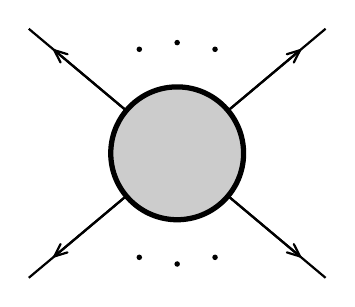
\begin{tikzpicture}[scale=1]
  \fill[black,opacity=0.20] (0,0) circle (24pt);
  \draw[line width=1.9pt] (0,0) circle (24pt);

  \draw[line width=0.8pt] (220:24pt) -- (220:70pt);
  \draw[->,>=angle 45,line width=0.8pt] (220:24pt) -- (220:59pt);

  \draw[line width=0.8pt] (140:24pt) -- (140:70pt);
  \draw[->,>=angle 45,line width=0.8pt] (140:24pt) -- (140:59pt);

  % dots
  \fill[] (90:40pt)circle (1.0pt);
  \fill[] (110:40pt)circle (1.0pt);
  \fill[] (70:40pt)circle (1.0pt);

  \draw[line width=0.8pt] (40:24pt) -- (40:70pt); % node[right] { $\Phi_{i-1}$};
  \draw[->,>=angle 45,line width=0.8pt] (40:24pt) -- (40:59pt);

  \draw[line width=0.8pt] (-40:24pt) -- (-40:70pt); % node[right] { $\Phi_{i+1}$};
  \draw[->,>=angle 45,line width=0.8pt] (-40:24pt) -- (-40:59pt);

  % dots
  \fill[] (-90:40pt)circle (1.0pt);
  \fill[] (-110:40pt)circle (1.0pt);
  \fill[] (-70:40pt)circle (1.0pt);

  \end{tikzpicture}

  \caption{An $n$-particle scattering amplitude.}
  \label{fig:n-particle-scattering-amplitude}
\end{figure}

As shown schematically in Figure \ref{fig:n-particle-scattering-amplitude}, for the sake of simplicity yet without sacrificing generality, it is assumed that all particles are outgoing. The on-shell condition for each external particle mandates that
\begin{align}
p_i^2 = 0, \quad i=1,\ldots,n.
\end{align}
Furthermore, due to the translation symmetry, the conservation of total momentum must be satisfied,
\begin{align}
\sum_{i=1}^{n} p_i^\mu = 0.
\end{align}

In general, the scattering amplitude is a scalar function of the momenta $p_i$
and the wavefunctions $\psi^I_i(p_i)$ (polarisation vectors and tensors) of external particles \cite{Boels:2016xhc,Boels:2017gyc,Peskin:1995ev,Cheung:2017pzi}. More preciously, the amplitude must be multi-linear in their external wavefunctions. For example, a gluon amplitude takes the form
\begin{align}
A_n = \epsilon_{1,\mu_1}\epsilon_{2,\mu_2}\cdots \epsilon_{n,\mu_n} I^{\mu_1\mu_2\cdots\mu_n}
\end{align}
This structure is quite manifest in the formalism of Feynman diagrams, which we will see examples of in the next chapter. Note that for a scalar particle, its wavefunction is completely determined by its momentum and thus, conventionally, can be equalled to unity. This reflects the fact that the amplitude of scalars is simply a function of the momenta:
\begin{align}
A_{\text{scalar}} = A(p_1,\ldots,p_n)
\end{align}
The transversality principle states that any polarization vector is orthogonal to its corresponding momentum vector, which can be represented as 
\begin{align}\label{chap2-transversality}
\epsilon_i(p_i) \cdot p_i = 0 \,.
\end{align}
According to the on-shell gauge invariance, for gluons, photons, or gravitons, the on-shell scattering amplitude vanishes when any polarization vector is substituted with its momentum:
\begin{align}\label{chap2-gauge-inv}
A(\epsilon_i^\mu \to p_i^\mu) = 0 \,.
\end{align}
Bose symmetry implies that the scattering amplitude remains unchanged when the quantum numbers of two indistinguishable bosons (particles with integer spins) are interchanged.

Finally, the locality is manifested through the singularity structure of scattering amplitudes in kinematic variables. Specifically, at the tree level, the amplitude exhibits the singularity of a simple pole, $1/P^2$, occurring when an intermediate state goes on-shell, $P^2\to m^2$.



\newpage
\section{Quantum Field Theory}
\label{sec:quantum-field-theory}

In the previous chapter, we introduced the basic concepts of Lorentz symmetry, particles, and scattering amplitudes. In this chapter, we understand particles and S-matrix from the viewpoint of quantum field theory.

%This chapter focuses more on traditional QFT and Lagrangian methodology.
%Read also e.g \cite{Boels:2017gyc}

%\zl{Here the basic structure I suggested follows:} In chapter 2, we understand particles as the irreducible representations of the little group, then review the basic properties of the S-matrix for these particles scatter off each other. In this chapter, we understand particles and S-matrix from the viewpoint of quantum field theory/Lagrangian (Feynman diagrams). We first briefly introduce various fields, such as scalars, gauge vectors and gravitons (maybe also fermions) using the simplest theories, like $\lambda\phi^4$, pure Yang-Mills/QCD and Hilbert-Einstein gravity. Then once we have all building blocks of fields, we can show that one can construct higher-dimensional (EFT) operators.

%Then in the next chapter, we combine ideas from this and previous chapters to show our main methods/results.  

\subsection{Scalar fields}\label{subsec:scalar-fields}

We begin this chapter by looking at the scattering of scalar particles in the context of $\lambda\phi^3$-theory («phi-cubed»). The Lagrangian is given by
\begin{equation}
\label{eq:sec3:phi3-lagrangian}
	\mathcal{L} = \frac{1}{2}(\del_{\mu}\phi)^{2}-\frac{1}{2}m^{2}\phi^{2}-\frac{\lambda}{3!}\phi^{3} \,,
\end{equation}
with $(\del_{\mu}\phi)^2 \equiv \eta_{\mu\nu}\,\del^{\mu}\phi\,\del^{\nu}\phi$. The first two terms describe a free particle of mass $m$ propagating through space-time, and make up the Lagrangian of what is known as free Klein-Gordon (K-G) field theory. The last term in \eqref{eq:sec3:phi3-lagrangian} describes the interaction between fields, whose strength is characterized by a coupling constant, $\lambda$.

When the coupling constant $\lambda$ is sufficiently small, the theory can be solved iteratively using perturbation methods. This can be carried out using Feynman diagrams systematically. More precisely, we can read out the propagator of scalars in momentum space\footnote{Ignoring the $i\varepsilon$-prescription of Feynman \cite{Elvang:2015rqa}.},
\begin{align}
\label{eq:sec3:phi3-propagator}
    \Delta(p) &= \frac{i}{p^2-m^2}
\end{align}
from the free Klein-Gordon Lagrangian, and the three-scalar vertex,
\begin{align}
\label{eq:sec3:phi3-vertex}
    V_{\phi\phi\phi} &= -i\lambda \,,
\end{align}
from the interacting Lagrangian. As discussed earlier, the wavefunctions of external scalar lines can conventionally be considered unity, 1.

Focusing on massless particles, we omit the mass term from the propagator for simplicity. Roughly speaking, the scattering amplitude for a given process is given by summing over all possible diagrams, categorized by their number of closed loops. Specifically, the tree-level amplitude, i.e.~the leading order in the perturbative expansion, is given by diagrams of tree-like topology, which have no closed loops. See any standard textbook for details, e.g.~\cite{Peskin:1995ev,Weinberg:1995mt}.

We now proceed to calculate the tree-level scattering amplitudes for four scalar particles. Using \eqref{eq:sec3:phi3-propagator} and \eqref{eq:sec3:phi3-vertex}, we can construct Feynman diagrams. In this case, we get the three diagrams shown in Figure \ref{fig:sec3:4pt-stu-channel-diagrams}. Throughout the rest of this work we are working with all external momenta pointing outwards, as well as defining the Mandelstam invariants \cite{Mandelstam:1958xc} as ${s = (p_1+p_2)^2}$, ${t = (p_1+p_3)^2}$ and ${u = (p_1+p_4)^2}$ in every 4-particle scattering process.
\begin{figure}
    \centering
    \begin{subfigure}[b]{0.3\textwidth}
        \centering
        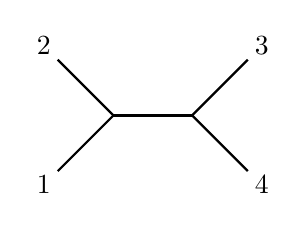
\begin{tikzpicture}
            \tikzset{line/.style={line width=0.8pt}};
            
            \draw[line] (-0.50,0) -- (0.50,0);
            
            \tikzset{shift={(-0.50,0)}};
            \node at (135:1.25) {2};
            \draw[line] (0,0) -- (135:1);
            \node at (225:1.25) {1};
            \draw[line] (0,0) -- (225:1);
            
            \tikzset{shift={(1,0)}};
            \node at (45:1.25) {3};
            \draw[line] (0,0) -- (45:1);
            \node at (315:1.25) {4};
            \draw[line] (0,0) -- (315:1);
        \end{tikzpicture}
        \caption{$s$-channel diagram.}
        \label{fig:sec3:4pt-s-channel-diagram}
    \end{subfigure}
    \begin{subfigure}[b]{0.3\textwidth}
        \centering
	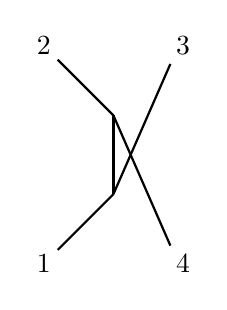
\begin{tikzpicture}
            \tikzset{line/.style={line width=0.8pt}};
            
            \draw[line] (0,0.50) -- (0,-0.50);
            
            \tikzset{shift={(0,-0.5)}};
            
            \node at (225:1.25) {1};
            \draw[line] (0,0) -- (225:1);
            \node (4) at (315:1.1) {};
            \node at (315:1.25) {4};
            
            \tikzset{shift={(0,1)}};
            
            \node at (135:1.25) {2};
            \draw[line] (0,0) -- (135:1);
            
            \node at (45:1.25) {3};
            \node (3) at (45:1.1) {};
            
            \draw[line] (0,0) -- (4);
            
            \tikzset{shift={(0,-1)}};
            
            \draw[line] (0,0) -- (3);
        \end{tikzpicture}
        \caption{$t$-channel diagram.}
        \label{fig:sec3:4pt-t-channel-diagram}
    \end{subfigure}
    \begin{subfigure}[b]{0.3\textwidth}
        \centering
        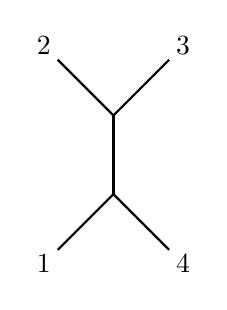
\begin{tikzpicture}
            \tikzset{line/.style={line width=0.8pt}};
            
            \draw[line] (0,0.50) -- (0,-0.50);
            
            \tikzset{shift={(0,-0.5)}};
            \node at (225:1.25) {1};
            \draw[line] (0,0) -- (225:1);
            \node at (315:1.25) {4};
            \draw[line] (0,0) -- (315:1);
            
            \tikzset{shift={(0,1)}}
            \node at (135:1.25) {2};
            \draw[line] (0,0) -- (135:1);
            \node at (45:1.25) {3};
            \draw[line] (0,0) -- (45:1);
        \end{tikzpicture}
        \caption{$u$-channel diagram.}
        \label{fig:sec3:4pt-u-channel-diagram}
    \end{subfigure}
    \caption{Schematical diagrams contributing to the scattering process, $1+2 \rightarrow 3+4$, at tree level.}
    \label{fig:sec3:4pt-stu-channel-diagrams}
\end{figure}
Each of the diagrams in Figure \ref{fig:sec3:4pt-stu-channel-diagrams} is translated to an expression using \eqref{eq:sec3:phi3-propagator} and \eqref{eq:sec3:phi3-vertex}. The value of the diagram in e.g. Figure \ref{fig:sec3:4pt-s-channel-diagram} is equal to
\begin{equation}
 iA_{\phi\phi\phi\phi}^s = V_{\phi\phi\phi}\,\Delta(P_{12})\,V_{\phi\phi\phi} = -\frac{i\lambda^2}{s-m^2} \,,
\end{equation}
where $P_{ij} \equiv p_i + p_j$. Repeating for the remaining two diagrams and summating, we get the full amplitude expression given by
\begin{equation}
\label{eq:sec3:phi3-amplitude}
\begin{split}
    A_{\phi\phi\phi\phi} ={}& A_{\phi\phi\phi\phi}^s + A_{\phi\phi\phi\phi}^t + A_{\phi\phi\phi\phi}^u \\
    ={}& -\frac{\lambda^2}{s-m^2} - \frac{\lambda^2}{t-m^2} - \frac{\lambda^2}{u-m^2} \\
    ={}& -\lambda^2\biggl(\frac{1}{s-m^2}+\frac{1}{t-m^2}+\frac{1}{u-m^2}\biggr) \,.
\end{split}
\end{equation}
It is easy to see that \eqref{eq:sec3:phi3-amplitude} exhibits both Bose symmetry and locality. The amplitude in the massless case is obtained by taking the $m \rightarrow 0$ limit of \eqref{eq:sec3:phi3-amplitude}.

Using dimensional analysis, in which, as usual, $\hbar = c = 1$, we can deduce\footnote{Given a Lagrangian of the form $\mathcal{L}_{\phi^n} = \mathcal{L}_{\text{K-G}}-\frac{\lambda_n}{n!}\phi^n$, the dimension of the coupling constant is $[\lambda_n] = D - \frac{1}{2}n(D-2)$ \cite{Srednicki:2007qs}.} that the coupling constant is dimensionless in $D = 6$ space-time dimensions and has mass dimension 2 in $D = 4$. In the perturbative regime, field theories with mass dimension of the coupling constant bigger or equal to zero are especially convenient to work with. This is essentially because of the renormalisability condition \cite{Peskin:1995ev}. In fact, phi-cubed theory is one of only two renormalisable scalar field theories\footnote{The other being $\lambda\phi^4$-theory («phi-fourth»), most notably part of the description of the Higgs field \cite{Peskin:1995ev}. We note that the phi-fourth coupling constant is dimensionless in $D=4$.}. If the dimension of the coupling constant of a theory is non-zero, it is (usually) either ill- or trivially defined in the high energy limit. The latter occurs when the coupling constant has a positive mass dimension, as it scales inversely with energy. On the other hand, if the mass dimension of the coupling constant is negative, the theory explodes in the high energy limit. As we will see in Section \ref{subsec:graviton-fields}, this is highly relevant for the perturbative expansion of Einstein-Hilbert gravity.

\subsection{Gauge fields}\label{subsec:gauge-fields}

In this section we introduce gauge symmetry starting with the Abelian gauge symmetry of Quantum electrodynamics (QED), then extending this to the non-Abelian case of Yang-Mills theory.

\subsubsection*{Gauge symmetry}

We start by considering a fermionic field that transforms under a local\footnote{Meaning space-time dependent.} $\operatorname{U}(1)$ symmetry:
\begin{equation}
\label{eq:sec3:u(1)-fermionic-field-transformation}
    \psi(x) \rightarrow \psi'(x) = U(x)\psi(x) \,, \quad U(x) = U(\alpha(x)) = e^{i\alpha(x)}
\end{equation}
Here, $U(\alpha)$ is an element of the Abelian group $\operatorname{U}(1)$, and $\alpha(x)$ is a local phase change. We also introduce the gauge covariant derivate,
\begin{equation}
\label{eq:sec3:u(1)-covariant-derivative}
    D_{\mu} \equiv \del_{\mu} - igA_{\mu} \,,
\end{equation}
where $g$ is a coupling constant and $A_{\mu}(x)$ is a vector field, also called gauge field. The covariant derivate of the field transforms similar to the field itself,
\begin{equation}
    D_{\mu}\psi(x) \rightarrow \bigl(D_{\mu}\psi(x)\bigr)' = U(x)D_{\mu}\psi(x) \,,
\end{equation}
as long as the gauge field transforms according to
\begin{equation}
\label{eq:sec3:u(1)-gauge-field-transformation}
    A_{\mu}(x) \rightarrow A'_{\mu}(x) = A_{\mu} + \frac{1}{g}\del_{\mu}\alpha(x) \,.
\end{equation}
The second term in \eqref{eq:sec3:u(1)-gauge-field-transformation} manifests the gauge ``freedom'' of the field, as the space-dependent parameter $\alpha$ can be arbitrarily chosen. We also define an antisymmetric field tensor in terms of \eqref{eq:sec3:u(1)-covariant-derivative},
\begin{equation}
\label{eq:sec3:abelian-antisymmetric-field-tensor}
    F_{\mu\nu} \equiv \frac{i}{g}[D_{\mu},D_{\nu}] = \del_{\mu}A_{\nu} - \del_{\nu}A_{\mu} \,,
\end{equation}
which is invariant under \eqref{eq:sec3:u(1)-gauge-field-transformation}. Now it is clear that we can construct a gauge-invariant Lagrangian for the gauge field using \eqref{eq:sec3:abelian-antisymmetric-field-tensor}. The simplest such Lagrangian (in four space-time dimensions or less \cite{Cheng:1984vwu}) is
\begin{equation}
\label{eq:sec3:u(1)-gauge-invariant-term}
    \mathcal{L} = -\frac{1}{4}F_{\mu\nu}F^{\mu\nu} \,.
\end{equation}
In the context of quantum electrodynamics, the gauge field describes a massless spin-1 particle known as the photon. The antisymmetric tensor with coupling constant $e$, the electric charge, is recognised as the electromagnetic field tensor.

\subsubsection*{Yang-Mills}

% When extending QED to multiple fermionic fields, we are led to the non-Abelian gauge theory known as Yang-Mills theory (YM) \cite{Yang:1954ek}. \zl{This is not so correct, but... the main difference is the gauge group --  abelian and non-abelian. Abelian gauge field (Maxwell) can also couple to a multiplet of matter fields, which transforms under a higher-dimensional representation of $U(1)$.} Here we will treat the case of $N$ fermionic fields, in which we work in the $\operatorname{SU}(N)$ gauge group compared to the previous $\operatorname{U}(1)$ group.

% Yang-Mills theory (YM) is a non-abelian gauge theory based on the special unitary group $\operatorname{SU}(N)$. When combined with Dirac's theory it describes the interaction between the massive fermions and massless gauge bosons we know as, respectively, quarks and gluons, which makes it an integral part of the standard model.

% The main difference between QED and YM is the inclusion of multiple fermionic fields. This means that instead of working with a a single field transforming through $\operatorname{U}(1)$ phase factors, as in \eqref{eq:sec3:u(1)-fermionic-field-transformation}, we have an $N$-dimensional multiplet of fields that transforms into eachother by the means of unitary ${N \times N}$ matrices, which are elements of the special unitary group ${\operatorname{SU}(N)}$\footnote{$\operatorname{SU}(N)$ is obtained by removing the subgroup $\operatorname{U}(1)$ from $\operatorname{U}(N)$.} \cite{Peskin:1995ev}. In the following we will extend the discussion from the previous section and as usual our focus will be on the massless gauge bosons in the theory.

Yang-Mills theory (YM) is a non-abelian gauge theory based on the special unitary group $\operatorname{SU}(N)$\footnote{$\operatorname{SU}(N)$ is obtained by removing the subgroup $\operatorname{U}(1)$ from $\operatorname{U}(N)$.}. When combined with Dirac's theory it describes the interaction between the massive fermions and massless gauge bosons we know as, respectively, quarks and gluons, which makes it an integral part of the standard model. In the following we will extend the discussion from the previous section, deriving Feynman rules and compute scattering amplitudes. As usual, our focus will be on the massless gauge bosons in the theory.

We  consider the local transformation of multiple fermionic fields organised in an $N$-dimensional multiplet,
\begin{equation}
\label{eq:sec3:fermionic-multiplet}
    \Psi(x) =
    \begin{pmatrix}
        \psi_{1}(x) \\
        \vdots \\
        \psi_{N}(x) \\
    \end{pmatrix} \,.
\end{equation}
These fields transform into eachother by the means of unitary ${N{\times}N}$ matrices, which are elements of the $\operatorname{SU}(N)$ \cite{Peskin:1995ev}. The transformation of \eqref{eq:sec3:fermionic-multiplet} is given by
\begin{equation}
    \psi_{i}(x) \rightarrow \psi'_{i}(x) = [U(x)]_{i}{}^{j}\,\psi_{j}(x) \,, \quad U(x) = U(\alpha(x)) = e^{i\alpha^{a}(x)T^{a}} \,,
\end{equation}
where $\alpha^a$ are real constants and the matrices $T^a$, $a\in\{1,2,\ldots, N^2 {-} 1\}$, are the fundamental representations of the generators of $\operatorname{SU}(N)$. The generators are normalised according to
\begin{equation}
\label{eq:sec3:su(n)-generators-normalisation}
    \tr(T^{a}T^{b}) = \delta^{ab} \,,
\end{equation}
and satisfy the commutation relation
\begin{equation}
\label{eq:sec3:su(n)-commutation-relation}
[T^a,T^b] = i\sqrt{2}f^{abc}T^c \,,
\end{equation}
where $f^{abc}$ are the structure constants of the group, defining the $\operatorname{SU}(N)$ Lie algebra.
The covariant derivative naturally extends from \eqref{eq:sec3:u(1)-covariant-derivative} to
\begin{equation}
\label{eq:sec3:ym-covariant-derivative}
    D_{\mu} \equiv \del_{\mu} - igA_{\mu} \,, \quad A_{\mu} \equiv A_{\mu}^{a\:}T^{a} \,,
\end{equation}
with $A_{\mu}(x)$ a matrix valued gauge-field. The transformation rule for the covariant derivative,
\begin{equation}
    D_{\mu}\psi(x) \rightarrow \bigl(D_{\mu}\psi(x)\bigr)' = U(x)D_{\mu}\psi(x) \,,
\end{equation}
dictates that the gauge field to transforms according to
\begin{equation}
     A_{\mu}(x) \rightarrow A'_{\mu}(x) = U(x)A_{\mu}(x)U^{-1}(x) - \frac{i}{g}\bigl(\del_{\mu}U(x)\bigr)U^{-1}(x) \,.
\end{equation}
As in the previous section we can define an antisymmetric field tensor using the covariant derivate:
\begin{equation}
\label{eq:sec3:non-abelian-antisymmetric-field-tensor}
    F_{\mu\nu} \equiv \frac{i}{g}[D_{\mu},D_{\nu}] = \del_{\mu}A_{\nu} - \del_{\nu}A_{\mu} - \frac{ig}{\sqrt{2}}[A_{\mu},A_{\nu}] = F_{\mu\nu}^{a}T^{a}
\end{equation}
Here,
\begin{equation}
\label{eq:sec3:non-abelian-antisymmetric-field-tensor-adjoint}
    F_{\mu\nu}^{a} = \del_{\mu}A_{\nu}^{a} - \del_{\nu}A_{\mu}^{a} + gf^{abc}A_{\mu}^{b\:}A_{\nu}^{c} \,.
\end{equation}
Now, with the help of \eqref{eq:sec3:non-abelian-antisymmetric-field-tensor} we can construct a gauge-invariant Lagrangian for the gauge field:
\begin{equation}
\label{eq:sec3:ym-lagrangian}
    \mathcal{L} = -\frac{1}{4}\tr\bigl(F_{\mu\nu}F^{\mu\nu}\bigr) = -\frac{1}{4}F_{\mu\nu}^{a}F^{a\mu\nu}
\end{equation}
This is recognised as the YM Lagrangian.

To derive Feynman rules from \eqref{eq:sec3:ym-lagrangian}, we expand it:
\begin{equation}
\label{eq:sec3:ym-lagrangian-expanded}
    \mathcal{L} = -\frac{1}{2}\del_{\mu}A_{\nu}^{a\:}(\del^{\mu}A^{a\nu} - \del^{\nu}A^{a\mu}) -\frac{g}{2}f^{abc}(\del_{\mu}A_{\nu}^{a} - \del_{\nu}A_{\mu}^{a})A^{b\mu}A^{c\nu} - \frac{g^2}{4}f^{abe}f^{ecd}A_{\mu}^{a\:}A_{\nu}^{b\:}A^{c\mu}A^{d\nu}
\end{equation}
We identify two vertices, linearly and quadratically proportional to the coupling constant, which is translated to
\begin{align}
\label{eq:sec3:su(n)-cubic-vertex}
    V_{ggg}^{a_1 a_2 a_3 \mu_1 \mu_2 \mu_3}(p_1,p_2,p_3) ={}& igf^{a_{1}a_{2}a_{3}}\bigl(\eta^{\mu_{1}\mu_{2}}(p_1-p_2)^{\mu_{3}}+\eta^{\mu_{2}\mu_{3}}(p_2-p_3)^{\mu_{1}}+\eta^{\mu_{3}\mu_{1}}(p_3-p_1)^{\mu_{2}}\bigr) \\
\intertext{and}
\label{eq:sec3:su(n)-quartic-vertex}
    \begin{split}
        V_{gggg}^{a_1 \cdots a_4 \mu_1 \cdots \mu_4}(p_1,\dots,p_4) ={}& - ig^2\bigl[f^{a_{1}a_{2}b}f^{b\,a_{3}a_{4}}(\eta^{\mu_{1}\mu_{4}}\eta^{\mu_{2}\mu_{3}} - \eta^{\mu_{1}\mu_{3}}\eta^{\mu_{2}\mu_{4}}) \\
	{}&+ f^{a_{1}a_{3}b}f^{b\,a_{2}a_{4}} (\eta^{\mu_{1}\mu_{2}}\eta^{\mu_{3}\mu_{4}} - \eta^{\mu_{1}\mu_{3}}\eta^{\mu_{2}\mu_{4}}) \\
	{}&+ f^{a_{1}a_{4}b}f^{b\,a_{2}a_{3}} (\eta^{\mu_{1}\mu_{2}}\eta^{\mu_{3}\mu_{4}} - \eta^{\mu_{1}\mu_{4}}\eta^{\mu_{2}\mu_{3}})\bigr]
    \end{split}
\end{align}
respectively. To derive the propagator between two gauge fields, we must fix the gauge field. This is traditionally done via the Fadeev-Popov method \cite{Peskin:1995ev}, in which one introduces anti-commuting fields, called ghosts, that appears inside loops. For our purposes we note that one can add a gauge-fixing term to the Lagrangian in \eqref{eq:sec3:ym-lagrangian}. There are a family of such terms, known as $R_{\xi}$ gauges \cite{Srednicki:2007qs}:
\begin{equation}
    \label{eq:sec3:r-xi-gauge-family}
    \mathcal{L}_{\mathrm{gf}}(\xi) = -\frac{1}{2\xi}\del^{\mu}A_{\mu}^{a\:}\del^{\nu}A_{\nu}^{a}
\end{equation}
Setting $\xi = 1$ gives the Feynman-'t Hooft gauge. Adding this to \eqref{eq:sec3:ym-lagrangian-expanded}, the terms involving two derivatives of the field looks like:
\begin{equation}
    \mathcal{L}_{A^2} = -\frac{1}{2}\bigl(\del_{\mu}A_{\nu}^{a\:}\del^{\mu}A^{a\nu} - \del_{\mu}A_{\nu}^{a\:}\del^{\nu}A^{a\mu} + \del_{\mu}A^{a\mu}\del_{\nu}A^{a\nu}\bigr)
\end{equation}
Doing some integrations-by-parts, the last two terms cancel eachother and the resulting term becomes
\begin{equation}
    \mathcal{L}_{A^2} = \frac{1}{2}A_{\mu}^{a\:}\del^{2}A^{a\mu} \,.
\end{equation}
Now it is clear that the propagator takes the form
\begin{equation}
\label{eq:sec3:su(n)-propagator}
    \Delta_{\mu\nu}^{ab}(p) = -\delta^{ab}\frac{i\eta_{\mu\nu}}{p^2} \,.
\end{equation}
We present an alternative method of gauge-fixing in Appendix \ref{sec:gervais-neveu-gauge} that affects the three- and four-point vertices as well as the propagator, further simplifying the Feynman rules.

Inspecting the commutation relation \eqref{eq:sec3:su(n)-commutation-relation}, we see that we can express the structure constants purely in terms of the generators of the group:
\begin{equation}
\label{eq:sec3:su(n)-structure-constant-trace}
    i\sqrt{2}f^{abc} = \tr(T^{a}T^{b}T^{c})-(T^{a}T^{c}T^{b}) = \tr\bigl(T^a[T^b,T^c]\bigr)
\end{equation}
When constructing amplitudes using \eqref{eq:sec3:su(n)-cubic-vertex} and \eqref{eq:sec3:su(n)-quartic-vertex}, we see that they involve products of traces that shares a colour index. One can gather these types of products of traces into one single trace using the Fierz identity \cite{Dixon:2015der}:
\begin{equation}
\label{eq:sec3:fierz-identity}
    (T^{a})_{i}{}^{j}(T^{a})_{k}{}^{l} = \delta_{i}{}^{l}\delta_{k}{}^{j} - \frac{1}{N}\delta_{i}{}^{j}\delta_{k}{}^{l}
\end{equation}
We demonstrate how one of the trace products appearing in $f^{abe}f^{ecd}$ can be ``Fierz'ed'':
\begin{equation}
    \begin{aligned}
        \tr(T^{a}T^{b}T^{e})\tr(T^{e}T^{c}T^{d}) &= (T^{a})_{i}{}^{j}(T^{b})_{j}{}^{k}(T^{e})_{k}{}^{i}(T^{e})_{l}{}^{m}(T^{c})_{m}{}^{n}(T^{d})_{n}{}^{l} \\
        &= (T^{a})_{i}{}^{j}(T^{b})_{j}{}^{k}(\delta_{k}{}^{m}\delta_{l}{}^{i} - \frac{1}{N}\delta_{k}{}^{i}\delta_{l}{}^{m})(T^{c})_{m}{}^{n}(T^{d})_{n}{}^{l} \\
        &= \tr(T^{a}T^{b}T^{c}T^{d}) - \frac{1}{N}\delta^{ab}\delta^{cd}
    \end{aligned}
\end{equation}
Repeating this exercise for each of the trace products, the $\frac{1}{N}$ terms will cancel eachother out and we end up with
\begin{equation}
    \label{eq:sec3:su(n)-contact-trace}
    \begin{aligned}
        (i\sqrt{2})^{2}f^{abe}f^{ecd} &= -\tr(T^{a}T^{b}T^{c}T^{d}) + \tr(T^{a}T^{b}T^{d}T^{c}) +\tr(T^{a}T^{c}T^{d}T^{b}) - \tr(T^{a}T^{d}T^{c}T^{b}) \\
        &= -\tr\bigl([T^a,T^b][T^c,T^d]\bigr) \,.
    \end{aligned}
\end{equation}
% Inserting \eqref{eq:sec3:su(n)-structure-constant-as-traces} and \eqref{eq:sec3:su(n)-contact-trace} into \eqref{eq:sec3:ym-lagrangian-expanded} and inspecting the single- and zero-derivative terms, we 
% \begin{equation}
%     \begin{gathered}
%         \mathcal{L}_{1\del+2\del} = \frac{ig}{2\sqrt{2}}\del_{\mu}A_{\nu}^{a\:}A^{b\mu}A^{c\nu}\tr\bigl(T^a[T^{b},T^{c}]\bigr) - \frac{g^2}{8}A_{\mu}^{a\:}A_{\nu}^{b\:}A^{c\mu}A^{d\nu}\tr\big([T^a,T^b][T^c,T^d]\bigr)
%     \end{gathered}
% \end{equation}
Now, it is clear that any amplitude derived from \eqref{eq:sec3:ym-lagrangian-expanded}, with \eqref{eq:sec3:su(n)-structure-constant-trace} and \eqref{eq:sec3:su(n)-contact-trace} inserted, can be reduced to a sum of single traces over the generators. This leads to the colour decomposition of tree amplitudes \cite{Berends:1987cv,Mangano:1988kk}:
\begin{equation}
\label{eq:sec3:tree-amplitude-colour-decomposition}
    \mathcal{A}_{n} = g^{n-2}\sum_{\sigma\in{S_n/Z_n}}\tr(T^{a_{\sigma(1)}}\cdots{T^{a_{\sigma(n)}}})A_{n}(\sigma(1),\dots,\sigma(n)) \,,
\end{equation}
where the gauge coupling constant is not included in the partial amplitudes, $A_{n}$. The ordering of external legs, $\sigma$, is taken to be the permutations of $n$ objects modulo all cyclic permutations, reflecting the cyclicity of the generator traces.

The partial amplitudes satisfy a set of relations that reduces the number of independent basis partial amplitudes. There are three relations that reduces the number of basis partial amplitudes from $n!$ to $(n-3)!$, of which the first is cyclic-, and reflection invariance \cite{Bern:2008qj}:
\begin{equation}
\label{eq:sec3:cyclic-reflection-invariance}
    A_n(1,2,\dots,n) = A_n(2,\dots,n,1) \,, \quad A_n(1,2,\dots,n) = (-1)^n A_n(n,\dots,2,1)
\end{equation}
This is saying that only the overall cyclic order of the partial amplitude matters, not where the order is read off from. Next, we have the Kleiss-Kuijf relations given by \cite{Weinzierl:2016bus}:
\begin{equation}
\label{eq:sec3:kk-relations}
    A_n(1,\{\alpha\},n,\{\beta\}) = (-1)^{|\beta|}\sum_{\sigma\in\{\alpha\}\shuffle\{\beta\}^T}A_n(1,\{\sigma\},n)
\end{equation}
Here, $|\beta|$ is the length of the set $\{\beta\}$ and the sum is taken over all shuffles between $\{\alpha\}$ and $\{\beta\}^T$; the set of permutations preserving the relative ordering within the two subsets. The superscripted $T$ denotes the reversal of the ordering of $\{\beta\}$. Lastly, there is the well known BCJ relations, which can be written as \cite{Bern:2019prr}
\begin{equation}
\label{eq:sec3:bcj-relations}
    \sum_{i=2}^{n-1}p_1\cdot(p_2+\dots+p_i)A_n(2,\dots,i,1,i+1,\dots,n) = 0 \,.
\end{equation}
As stated above, when combining \eqref{eq:sec3:cyclic-reflection-invariance}, \eqref{eq:sec3:kk-relations} and \eqref{eq:sec3:bcj-relations} any $n$-point colour-ordered amplitude can be written in terms of $(n-3)!$ independent basis partial amplitudes \cite{Bjerrum-Bohr:2009ulz}. As a consequence, in both the 3- and 4-point case, only one basis amplitude is needed. These will be computed in the following.

We can now write down colour-ordered Feynman rules for the partial amplitudes. The cubic vertex is the same as in \eqref{eq:sec3:su(n)-cubic-vertex} with the replacement $gf^{abc}\rightarrow\frac{1}{\sqrt{2}}$ and the quartic vertex is simplified significantly \cite{Dixon:1996wi}:
\begin{align}
    \label{eq:sec3:colour-ordered-qubic-vertex}
    \begin{split}
        V_{ggg}^{\mu_1 \mu_2 \mu_3}(p_1,p_2,p_3) ={}& \frac{i}{\sqrt{2}}\bigl(\eta^{\mu_{1}\mu_{2}}(p_1-p_2)^{\mu_{3}}+\eta^{\mu_{2}\mu_{3}}(p_2-p_3)^{\mu_{1}} \\
        {}&+ \eta^{\mu_{3}\mu_{1}}(p_3-p_1)^{\mu_{2}}\bigr)
    \end{split} \\[2ex]
    \label{eq:sec3:colour-ordered-quartic-vertex}
    V_{gggg}^{\mu_1 \cdots \mu_4}(p_1,\dots,p_4) ={}& \frac{i}{2}\bigl(2\eta^{\mu_{1}\mu_{3}}\eta^{\mu_{2}\mu_{4}}-\eta^{\mu_{1}\mu_{2}}\eta^{\mu_{3}\mu_{4}}-\eta^{\mu_{1}\mu_{4}}\eta^{\mu_{2}\mu_{3}}\bigr)
\end{align}
In addition, the propagator is written without the colour-indexed Kronecker delta in \eqref{eq:sec3:su(n)-propagator}, namely
\begin{equation}
    \Delta_{\mu\nu}(p) = -\frac{i\eta_{\mu\nu}}{p^2} \,.
\end{equation}
The colour-ordered three-point amplitude is easily computed by contracting three external polarisation vectors to the vertex in \eqref{eq:sec3:su(n)-cubic-vertex} with the aforementioned replacement. We denote the cubic vertex by $V_{ggg}^{\mu\nu\rho}(p,k,l)$, where the momenta in the parantheses belongs to the leg with corresponding Lorentz index:
\begin{equation}
    \begin{split}
        i A_{ggg}(1,2,3) ={}& {\epsilon_{1}}_{\mu_{1}}{\epsilon_{2}}_{\mu_{2}}{\epsilon_{3}}_{\mu_{3}}V_{ggg}^{\mu_{1}\mu_{2}\mu_{3}}(p_1,p_2,p_3) \\
        ={}& \frac{i}{\sqrt{2}}\bigl[(\epsilon_{1}\cdot\epsilon_{2})(\epsilon_{3}\cdot{p_{1}}) - (\epsilon_{1}\cdot\epsilon_{2})(\epsilon_{3}\cdot{p_{2}}) + (\epsilon_{2}\cdot\epsilon_{3})(\epsilon_{1}\cdot{p_{2}}) \\
        {}&- (\epsilon_{2}\cdot\epsilon_{3})(\epsilon_{1}\cdot{p_{3}}) + (\epsilon_{3}\cdot\epsilon_{1})(\epsilon_{2}\cdot{p_{3}}) - (\epsilon_{3}\cdot\epsilon_{1})(\epsilon_{2}\cdot{p_{1}})\bigr]
    \end{split}
\end{equation}

We would now like to compute the value of the four-point gauge-field amplitude using the colour-ordered Feynman rules. There are three diagrams contributing to the amplitude. Two of the diagrams are the familiar $s$- and $u$-channel diagrams. The $t$-channel diagram is excluded because of colour-ordering. In addition there is a contributing contact diagram shown, schematically, in Figure~\ref{fig:sec3:4pt-contact-diagram}.
% \begin{figure}
%     \centering
%     \begin{subfigure}[b]{0.3\textwidth}
%         \centering
%         \begin{tikzpicture}[scale=1]
%             \tikzset{line/.style={line width=0.8pt}};
            
%             \draw[line] (-0.50,0) -- (0.50,0);
            
%             \tikzset{shift={(-0.50,0)}};
%             \node at (135:1.25) {2};
%             \draw[line] (0,0) -- (135:1);
%             \node at (225:1.25) {1};
%             \draw[line] (0,0) -- (225:1);
            
%             \tikzset{shift={(1,0)}};
%             \node at (45:1.25) {3};
%             \draw[line] (0,0) -- (45:1);
%             \node at (315:1.25) {4};
%             \draw[line] (0,0) -- (315:1);
%         \end{tikzpicture}
%         \caption{$s$-channel diagram.}
%         \label{fig:sec3:su(n)-s-channel-diagram}
%     \end{subfigure}
%     \begin{subfigure}[b]{0.3\textwidth}
%         \centering
%         \begin{tikzpicture}[scale=1]
%             \tikzset{line/.style={line width=0.8pt}};
            
%             \draw[line] (0,0.50) -- (0,-0.50);
            
%             \tikzset{shift={(0,-0.5)}};
%             \node at (225:1.25) {1};
%             \draw[line] (0,0) -- (225:1);
%             \node at (315:1.25) {4};
%             \draw[line] (0,0) -- (315:1);
            
%             \tikzset{shift={(0,1)}}
%             \node at (135:1.25) {2};
%             \draw[line] (0,0) -- (135:1);
%             \node at (45:1.25) {3};
%             \draw[line] (0,0) -- (45:1);
%         \end{tikzpicture}
%         \caption{$u$-channel diagram.}
%         \label{fig:sec3:su(n)-u-channel-diagram}
%     \end{subfigure}
%     \begin{subfigure}[b]{0.3\textwidth}
%         \centering
%         \begin{tikzpicture}[scale=1]
%             \tikzset{line/.style={line width=0.8pt}};
            
%             \node at (225:1.25) {1};
%             \draw[line] (0,0) -- (225:1);
%             \node at (315:1.25) {4};
%             \draw[line] (0,0) -- (315:1);
            
%             \node at (135:1.25) {2};
%             \draw[line] (0,0) -- (135:1);
%             \node at (45:1.25) {3};
%             \draw[line] (0,0) -- (45:1);
%         \end{tikzpicture}
%         \caption{Contact diagram}
%         \label{fig:sec3:su(n)-contact-diagram}
%     \end{subfigure}
%     \caption{The three diagrams contributing to the four-point colour-ordered gauge-field amplitude.}
%     \label{fig:sec3:4pt-colour-ordered-diagrams}
% \end{figure}
\begin{figure}
    \centering
    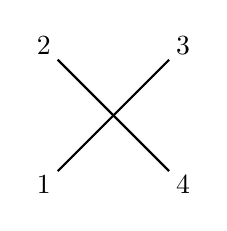
\begin{tikzpicture}[scale=1]
        \tikzset{line/.style={line width=0.8pt}};
        
        \node at (225:1.25) {1};
        \draw[line] (0,0) -- (225:1);
        \node at (315:1.25) {4};
        \draw[line] (0,0) -- (315:1);
        
        \node at (135:1.25) {2};
        \draw[line] (0,0) -- (135:1);
        \node at (45:1.25) {3};
        \draw[line] (0,0) -- (45:1);
    \end{tikzpicture}
    \caption{Contact diagram}
    \label{fig:sec3:4pt-contact-diagram}
\end{figure}
The $s$- and $u$-channel diagrams is then given by
\begin{align}
\label{eq:sec3:4pt-s-channel-expression}
    i A_{gggg}^{s}(1,2,3,4) &= {\epsilon_{1}}_{\mu_{1}}{\epsilon_{2}}_{\mu_{2}}{\epsilon_{3}}_{\mu_{3}}{\epsilon_{3}}_{\mu_{4}}V_{ggg}^{\mu_{1}\mu_{2}\nu}(p_1,p_2,P_{34})\Delta_{\nu\rho}(P_{12})V_{ggg}^{\rho\mu_{3}\mu_{4}}(P_{12},p_3,p_4) \\
\intertext{and}
\label{eq:sec3:4pt-u-channel-expression}
    i A_{gggg}^{u}(1,2,3,4) &= {\epsilon_{1}}_{\mu_{1}}{\epsilon_{2}}_{\mu_{2}}{\epsilon_{3}}_{\mu_{3}}{\epsilon_{3}}_{\mu_{4}}V_{ggg}^{\mu_{4}\mu_{1}\nu}(p_4,p_1,P_{23})\Delta_{\nu\rho}(P_{14})V_{ggg}^{\rho\mu_{2}\mu_{3}}(P_{14},p_2,p_3) \,.
\end{align}
The value of the contact diagram in Figure is simply the quartic vertex contracted with four polarisation vectors:
\begin{equation}
\label{eq:sec3:4pt-contact-expression}
    \begin{aligned}
        i A_{gggg}^{c}(1,2,3,4) &= \frac{i}{2}{\epsilon_{1}}_{\mu_{1}}{\epsilon_{2}}_{\mu_{2}}{\epsilon_{3}}_{\mu_{3}}{\epsilon_{3}}_{\mu_{4}}(2\eta^{\mu_{1}\mu_{3}}\eta^{\mu_{2}\mu_{4}}-\eta^{\mu_{1}\mu_{2}}\eta^{\mu_{3}\mu_{4}}-\eta^{\mu_{1}\mu_{4}}\eta^{\mu_{2}\mu_{3}}) \\[2ex]
        &= \frac{i}{2}\bigl[2(\epsilon_{1}\cdot\epsilon_{3})(\epsilon_{2}\cdot\epsilon_{4}) - (\epsilon_{1}\cdot\epsilon_{2})(\epsilon_{3}\cdot\epsilon_{4}) - (\epsilon_{1}\cdot\epsilon_{4})(\epsilon_{2}\cdot\epsilon_{3})\bigr] \,.
    \end{aligned}
\end{equation}
The full four-point amplitude is the sum of \eqref{eq:sec3:4pt-s-channel-expression}, \eqref{eq:sec3:4pt-u-channel-expression} and \eqref{eq:sec3:4pt-contact-expression} and is given by, dropping the explicit dot-notation for compactness,
\begin{equation}
\label{eq:sec3:4pt-ym-amplitude}
    \begin{split}
        A_{gggg}(1,2,3,4) ={}& A_{gggg}^{s}(1,2,3,4) + A_{gggg}^{u}(1,2,3,4) + A_{gggg}^{c}(1,2,3,4) \\[2ex]
        ={}&\frac{1}{s(s+t)}\Bigl(t(s+t)\ee{1}{2}\ee{3}{4} + s(s+t)\ee{1}{3}\ee{2}{4} - st\ee{1}{4}\ee{2}{3} \\[1ex]
        {}&+ 2s\bigl[\ee{1}{2}\ep{3}{1}\ep{4}{2} + \ee{1}{3}\ep{2}{3}\ep{4}{2} + \ee{1}{3}\ep{2}{1}\ep{4}{3} \\
        {}&+ \ee{1}{3}\ep{2}{3}\ep{4}{3} + \ee{1}{4}\ep{2}{1}\ep{3}{1} + \ee{1}{4}\ep{2}{3}\ep{3}{1} \\
        {}&- \ee{2}{3}\ep{1}{3}\ep{4}{2} - \ee{2}{4}\ep{1}{2}\ep{3}{1} + \ee{2}{4}\ep{1}{3}\ep{3}{2} \\
        {}&- \ee{3}{4}\ep{1}{3}\ep{2}{1} - \ee{3}{4}\ep{1}{3}\ep{2}{3}\bigr] \\[1ex]
        {}&+ 2t\bigl[\ee{1}{2}\ep{3}{1}\ep{4}{2} + \ee{1}{2}\ep{3}{2}\ep{4}{2} + \ee{1}{2}\ep{3}{2}\ep{4}{3} \\
        {}&+ \ee{1}{3}\ep{2}{1}\ep{4}{3} + \ee{1}{4}\ep{2}{1}\ep{3}{1} + \ee{1}{4}\ep{2}{1}\ep{3}{2} \\
        {}&- \ee{2}{3}\ep{1}{2}\ep{4}{3} - \ee{2}{4}\ep{1}{2}\ep{3}{1} - \ee{2}{4}\ep{1}{2}\ep{3}{2} \\
        {}&- \ee{3}{4}\ep{1}{3}\ep{2}{1} + \ee{3}{4}\ep{1}{2}\ep{2}{3}\bigr]\Bigr) \,.
    \end{split}
\end{equation}




\subsection{Einstein gravity}\label{subsec:graviton-fields}

%\begin{description}
%    \item [Einstein-Hilbert gravity]
%\end{description}

In the following we will consider the perturbative expansion of Einstein-Hilbert (EH) gravity. As is well known, the coupling constant of EH has positive mass dimension, and is thus not renormalisable in the scheme of perturbative QFT. However, when viewed as an effective field theory, meaning valid at low energies relative to the Planck scale, we are free to do computations in the same manner as in the previous section, deriving Feynman rules from a Lagrangian density.

%{\color{blue} here I consider building the Lagrangian from the commutator of the covariant derivative, mirroring the previous sections}
%
%In analogy with the discussion of gauge fields in the previous section, we consider now a massive scalar field, $\phi$, transforming under a local coordinate transformation:
%\begin{equation}
%    x^{\mu} \rightarrow x'^{\mu} = x^{\mu} + a^{\mu}(x) \,,
%\end{equation}
%This is known as a general coordinate transformation. 

The Einstein-Hilbert Lagrangian is given by
\begin{equation}
\label{eq:sec3:eh-lagrangian}
    \mathcal{L}_{\mathrm{EH}} = \frac{2}{\kappa^2}\sqrt{-g}R \,,
\end{equation}
where the coupling constant is $\kappa = \sqrt{32\pi{G}}$, $g_{\mu\nu}$ the metric tensor and $g = \det g_{\mu\nu}$. The square root-factor comes from the fact that $d^4x \sqrt{-g}$ is a well-defined measure, which is diffeomorphism invariant \cite{Donoghue:2017pgk}.
%a correction of the measure in the action integral,
%\begin{equation}
%    S=\int{d^{4}y\,\mathcal{L}} = \int{d^{4}x\,\sqrt{-g}\,\mathcal{L}} \,,
%\end{equation}
%when going to curved space. 
Here, we include the factor $\sqrt{-g}$ in the Lagrangian, avoiding a notation involving the action. $R = g^{\mu\nu}R_{\mu\nu}$ is the metric contraction of the Ricci tensor, also known as the scalar curvature. The Ricci tensor is given by \cite{Donoghue:1994dn}:
\begin{equation}
    R_{\mu\nu} = \del_{\nu}\Gamma_{\mu\lambda}^{\lambda} - \del_{\lambda}\Gamma_{\mu\nu}^{\lambda} + \Gamma_{\mu\lambda}^{\sigma}\Gamma_{\nu\sigma}^{\lambda} - \Gamma_{\mu\nu}^{\sigma}\Gamma_{\lambda\sigma}^{\lambda}
\end{equation}
Here, $\Gamma$ denotes the Christoffel symbol and is defined in terms of the metric by:
\begin{equation}
    \Gamma_{\nu\rho}^{\mu} = \frac{1}{2}g^{\mu\sigma}(\del_{\nu}g_{\sigma\rho} + \del_{\rho}g_{\sigma\nu} - \del_{\sigma}g_{\nu\rho})
\end{equation}
In the weak field limit, the metric can be parameterized as
\begin{equation}\label{matric-expansion}
    g_{\mu\nu} = \eta_{\mu\nu} + \kappa\,h_{\mu\nu} \,,
\end{equation}
where $\eta_{\mu\nu}$ is the flat metric and the second term is an exitation of Minkowski space, capturing any curvature in our space. We identify $h_{\mu\nu}$ with the graviton field. Then, the inverse metric is given by an expansion of the graviton field in powers of the coupling constant:
\begin{equation}
\label{eq:sec3:metric-expansion}
    g^{\mu\nu} = \eta^{\mu\nu} - \kappa\,h^{\mu\nu} + \kappa^2\,h^{\mu\rho}h_{\rho}{}^{\nu} - \kappa^3\,h^{\mu\rho}h_{\rho}{}^{\sigma}h_{\sigma}{}^{\nu} + \kappa^4\,h^{\mu\rho}h_{\rho}{}^{\sigma}h_{\sigma}{}^{\lambda}h_{\lambda}{}^{\nu} + \mathcal{O}(\kappa^5)
\end{equation}
Similarily, the expansion of $\sqrt{-g}$ is given by
\begin{equation}
    \sqrt{-g} = 1 + \frac{1}{2}\kappa\,h - \frac{1}{4}\kappa^2\Bigl((h_{\mu\nu})^2 - \frac{1}{2}h^2\Bigr) + \frac{1}{6}\kappa^3\Bigl(h_{\mu}{}^{\nu}h_{\nu}{}^{\rho}h_{\rho}{}^{\mu} - \frac{3}{4}h(h_{\mu\nu})^2 + \frac{1}{8}h^3\Bigr) + \mathcal{O}(\kappa^4) \,,
\end{equation}
where we have defined $h \equiv h_{\mu}{}^{\mu}$ and $(h_{\mu\nu})^2 \equiv h_{\mu\nu}h^{\mu\nu}$. The Lagrangian in \eqref{eq:sec3:eh-lagrangian} is invariant under the local  translation
\begin{equation}
    x^{\mu} \rightarrow x'^{\mu} = x^{\mu} + \xi^{\mu}(x) \,,
\end{equation}
which is known as a general coordinate transformation. This entails, to linear order, the following transformation for the graviton-field:
\begin{equation}
    h_{\mu\nu} \rightarrow h'_{\mu\nu} = h_{\mu\nu} + \del_{\mu}\xi_{\nu} + \del_{\nu}\xi_{\mu}
\end{equation}
This is a gauge transformation for the graviton field, thus indicating the necessity to add a gauge-fixing term to \eqref{eq:sec3:eh-lagrangian} in order to derive Feynman rules. One possible choice of gauge is the de Donder gauge \cite{Cheung:2020gyp}, given by
\begin{equation}
\label{eq:sec3:de-donder-gauge-fixing-term}
    \mathcal{L}_{\mathrm{gf}} = -\Big(\partial^\nu h_{\mu\nu} - \frac{1}{2}\del_{\mu}h\Big)^2 \,,
\end{equation}
where $h$ denotes the trace of the graviton field, $h \equiv \eta_{\mu\nu}h^{\mu\nu} = h_{\mu}{}^{\mu}$. Now, inserting the expansion \eqref{eq:sec3:metric-expansion} into the gauge fixed EH Lagrangian, we can order the resulting terms in powers of the coupling constant. This gives, schematically,
\begin{equation}
    \mathcal{L}_{\mathrm{EH}} = \mathcal{L}_{hh} + \mathcal{L}_{\mathrm{gf}} + \kappa\mathcal{L}_{hhh} + \kappa^2\mathcal{L}_{hhhh} + \mathcal{O}(\kappa^3) \,,
\end{equation}
where the order of the field in each term is given by the subscript. We note that the gauge-fix in \eqref{eq:sec3:de-donder-gauge-fixing-term} only affects the propagator, like we saw with the $R_\xi$-gauges in YM. Up to quadratic order in the coupling constant we get terms in the Lagrangian that produce a propagator, a cubic- and a quartic vertex. Most of the computations in the remaining part of this chapter have been done with the aid of \texttt{FeynRules} \cite{Alloul:2013bka}, a \textsc{Mathematica} package.

The gauge-fixed two-point Lagrangian is given by
\begin{equation}
\label{eq:sec3:lagrangian-propagator}
    \begin{split}
        % \mathcal{L}_{hh} ={}& 2 h^{\mu\nu} \del_{\nu}\del_{\mu}h^{\rho}{}_{\rho}-4 h^{\mu\nu} \del_{\nu}\del_{\rho}h_{\mu}{}^{\rho}- \frac{3}{4}\del_{\nu}h^{\rho}{}_{\rho} \del^{\nu}h^{\mu}{}_{\mu} -3 \del_{\mu}h^{\mu\nu} \del_{\rho}h_{\nu}{}^{\rho}+3 \del^{\nu}h^{\mu}{}_{\mu} \del_{\rho}h_{\nu}{}^{\rho} \\
        % {}&+ h^{\mu}{}_{\mu} \del_{\rho}\del_{\nu}h^{\nu\rho} + 2 h^{\mu\nu} \del_{\rho}\del^{\rho}h_{\mu\nu}-h^{\mu}{}_{\mu} \del_{\rho}\del^{\rho}h^{\nu}{}_{\nu}-\del_{\nu}h_{\mu\rho} \del^{\rho}h^{\mu\nu} + \frac{3}{2}\del_{\rho}h_{\mu\nu} \del^{\rho}h^{\mu\nu} \\
        \mathcal{L}_{hh} ={}& 2 h^{\mu\nu}\,\del_{\nu}\del_{\mu}h-4 h^{\mu\nu}\,\del_{\nu}\del_{\rho}h_{\mu}{}^{\rho}- \frac{3}{4}(\del_{\mu}h)^2 -3 \del_{\mu}h^{\mu\nu}\,\del_{\rho}h_{\nu}{}^{\rho}+3 \del^{\nu}h\,\del_{\rho}h_{\nu}{}^{\rho} \\
        {}&+ h\,\del_{\rho}\del_{\nu}h^{\nu\rho} + 2 h^{\mu\nu}\,\del^{2}h_{\mu\nu}-h\, \del^{2}h-\del_{\nu}h_{\mu\rho}\,\del^{\rho}h^{\mu\nu} + \frac{3}{2}(\del_{\mu}h_{\nu\rho})^{2} \\
        ={}&- 2 \del_{\nu}h^{\mu\nu}\,\del_{\mu}h + 4 \del_{\nu}h^{\mu\nu}\,\del_{\rho}h_{\mu}{}^{\rho}- \frac{3}{4}(\del_{\mu}h)^2 -3 \del_{\mu}h^{\mu\nu}\,\del_{\rho}h_{\nu}{}^{\rho}+3 \del^{\nu}h\,\del_{\rho}h_{\nu}{}^{\rho} \\
        {}&- \del_{\rho}h\,\del_{\nu}h^{\nu\rho} - 2 (\del_{\rho}h_{\mu\nu})^2 + (\del_{\mu}h)^{2} - \del^{\rho}h_{\mu\rho}\,\del_{\nu}h^{\mu\nu} + \frac{3}{2}(\del_{\mu}h_{\nu\rho})^{2} \\
        ={}& \frac{1}{4}(\del_{\mu}h)^2 - \frac{1}{2}(\del_{\mu}h_{\nu\rho})^2
    \end{split}
\end{equation}
To arrive at the last equality in \eqref{eq:sec3:lagrangian-propagator}, we perform some integrations-by-parts in the second equality, which makes it apparent that six of the terms vanish. Specifically, the first, fifth and sixth term sums to zero. The same goes for the second, fourth and ninth term. The remaining terms evaluates, after performing integration-by-parts on the seventh and eigth term, to the compact form given. The cubic Lagrangian is given by the following 28 terms:
%\\{\color{blue} Hi Zhengwen, the full form of the quartic Lagrangian should probably go in the appendix, maybe also the cubic Lagrangian.}\\
%\zl{Yes, to me, it's fine to display the 3-graviton here and put the 4-graviton to an appendix. But the 4-graviton is not very lengthy, so it's also not a problem if you want to present it in the main text here.}
\begin{equation}
    \begin{split}
        \mathcal{L}_{hhh} ={}& -\frac{3}{2}h^{\mu\nu}\,\del_{\mu}h^{\rho\sigma}\,\del_{\nu}h_{\rho\sigma}+\frac{1}{2}h^{\mu\nu}\,\del_{\mu}h\,\del_{\nu}h-2 h^{\mu\nu}\,\del_{\nu}h\,\del_{\rho}h_{\mu}{}^{\rho}-2 h^{\mu\nu}\,\del_{\nu}h_{\mu}{}^{\rho}\,\del_{\rho}h \\
        {}&-2 h_{\mu}{}^{\rho}\,h^{\mu\nu}\,\del_{\rho}\del_{\nu}h + h\,h^{\nu\rho}\,\del_{\rho}\del_{\nu}h + 4 h_{\mu}{}^{\rho}\,h^{\mu\nu}\,\del_{\rho}\del_{\sigma}h_{\nu}{}^{\sigma}-2 h\,h^{\nu\rho}\,\del_{\rho}\del_{\sigma}h_{\nu}{}^{\sigma} \\
        {}&+h^{\mu\nu}\,\del_{\rho}h\,\del^{\rho}h_{\mu\nu}-\frac{1}{4}h(\del_{\rho}h)^{2} + 2 h^{\mu\nu}\,\del_{\rho}h_{\mu}{}^{\rho}\,\del_{\sigma}h_{\nu}{}^{\sigma} + 4 h^{\mu\nu}\,\del_{\nu}h_{\mu}{}^{\rho}\,\del_{\sigma}h_{\rho}{}^{\sigma} \\
        {}&- h\,\del_{\nu}h^{\nu\rho}\,\del_{\sigma}h_{\rho}{}^{\sigma} - 2 h^{\mu\nu}\,\del^{\rho}h_{\mu\nu}\,\del_{\sigma}h_{\rho}{}^{\sigma} + h\,\del^{\rho}h\,\del_{\sigma}h_{\rho}{}^{\sigma} + 2 h^{\mu\nu}\,h^{\rho\sigma}\,\del_{\sigma}\del_{\nu}h_{\mu\rho} \\
        {}&- 2 h^{\mu\nu}\,h^{\rho\sigma}\,\del_{\sigma}\del_{\rho}h_{\mu\nu} - \frac{1}{2}h_{\mu\nu}\,h^{\mu\nu}\,\del_{\sigma}\del_{\rho}h^{\rho\sigma} + \frac{1}{4}h^{2}\,\del_{\sigma}\del_{\rho}h^{\rho\sigma} - 2 h_{\mu}{}^{\rho}\,h^{\mu\nu}\,\del^{2}h_{\nu\rho} \\
        {}&+ h\,h^{\nu\rho}\,\del^{2}h_{\nu\rho} + \frac{1}{2}(h_{\mu\nu})^{2}\,\del^{2}h - \frac{1}{4}h^{2}\,\del^{2}h + 2 h^{\mu\nu}\,\del_{\nu}h_{\rho\sigma}\,\del^{\sigma}h_{\mu}{}^{\rho} \\
        {}&+ h^{\mu\nu}\,\del_{\rho}h_{\nu\sigma}\,\del^{\sigma}h_{\mu}{}^{\rho} - 3 h^{\mu\nu}\,\del_{\sigma}h_{\nu\rho}\,\del^{\sigma}h_{\mu}{}^{\rho} - \frac{1}{2}h\,\del_{\rho}h_{\nu\sigma}\,\del^{\sigma}h^{\nu\rho} + \frac{3}{4}h\,\del_{\sigma}h_{\nu\rho}\,\del^{\sigma}h^{\nu\rho}
    \end{split}
\end{equation}
The quartic Lagrangian is given by 66 terms:
\begin{equation}
    \begin{split}
        \mathcal{L}_{hhhh} ={}&- h^{\mu\nu} h^{\rho\sigma}\,\del_{\nu}h_{\sigma\lambda}\,\del_{\rho}h_{\mu}{}^{\lambda}+ \frac{3}{2}h_{\mu}{}^{\rho} h^{\mu\nu}\,\del_{\nu}h^{\sigma\lambda}\,\del_{\rho}h_{\sigma\lambda}- \frac{3}{4}h\,h^{\nu\rho}\,\del_{\nu}h^{\sigma\lambda}\,\del_{\rho}h_{\sigma\lambda} \\
        {}&- \frac{1}{2}h_{\mu}{}^{\rho} h^{\mu\nu}\,\del_{\nu}h \del_{\rho}h+ \frac{1}{4}h\,h^{\nu\rho}\,\del_{\nu}h\,\del_{\rho}h + 2 h_{\mu}{}^{\rho} h^{\mu\nu} h^{\sigma\lambda}\,\del_{\rho}\del_{\nu}h_{\sigma\lambda} \\
        {}&- 4 h_{\mu}{}^{\rho} h^{\mu\nu} h^{\sigma\lambda}\,\del_{\rho}\del_{\lambda}h_{\nu\sigma}+2 h_{\mu}{}^{\rho} h^{\mu\nu}\,\del_{\rho}h\,\del_{\sigma}h_{\nu}{}^{\sigma}-h\,h^{\nu\rho}\,\del_{\rho}h\,\del_{\sigma}h_{\nu}{}^{\sigma} \\
        {}&+ 3 h^{\mu\nu} h^{\rho\sigma}\,\del_{\rho}h_{\mu}{}^{\lambda}\,\del_{\sigma}h_{\nu\lambda}-2 h^{\mu\nu} h^{\rho\sigma}\,\del_{\nu}h_{\mu}{}^{\lambda}\,\del_{\sigma}h_{\rho\lambda}+2 h^{\mu\nu} h^{\rho\sigma}\,\del_{\nu}h_{\mu\rho}\,\del_{\sigma}h \\
        {}&- h^{\mu\nu} h^{\rho\sigma}\,\del_{\rho}h_{\mu\nu}\,\del_{\sigma}h+2 h_{\mu}{}^{\rho} h^{\mu\nu}\,\del_{\rho}h_{\nu}{}^{\sigma}\,\del_{\sigma}h-h\,h^{\nu\rho}\,\del_{\rho}h_{\nu}{}^{\sigma}\,\del_{\sigma}h \\
        {}&+ 2 h_{\mu}{}^{\rho} h^{\mu\nu} h_{\nu}{}^{\sigma}\,\del_{\sigma}\del_{\rho}h-h\,h_{\nu}{}^{\sigma} h^{\nu\rho}\,\del_{\sigma}\del_{\rho}h- \frac{1}{2}(h_{\mu\nu})^{2} h^{\rho\sigma}\,\del_{\sigma}\del_{\rho}h \\
        {}&+ \frac{1}{4}h^{2}\,h^{\rho\sigma}\,\del_{\sigma}\del_{\rho}h -4 h_{\mu}{}^{\rho} h^{\mu\nu} h_{\nu}{}^{\sigma}\,\del_{\sigma}\del_{\lambda}h_{\rho}{}^{\lambda}+2 h\,h_{\nu}{}^{\sigma} h^{\nu\rho}\,\del_{\sigma}\del_{\lambda}h_{\rho}{}^{\lambda} \\
        {}&+ (h_{\mu\nu})^{2} h^{\rho\sigma}\,\del_{\sigma}\del_{\lambda}h_{\rho}{}^{\lambda}- \frac{1}{2}h^{2}\,h^{\rho\sigma}\,\del_{\sigma}\del_{\lambda}h_{\rho}{}^{\lambda}-h_{\mu}{}^{\rho} h^{\mu\nu}\,\del_{\sigma}h\,\del^{\sigma}h_{\nu\rho} \\
        {}&+ \frac{1}{2}h\,h^{\nu\rho}\,\del_{\sigma}h \del^{\sigma}h_{\nu\rho} + \frac{1}{8}(h_{\mu\nu})^{2}\,(\del_{\sigma}h)^{2} - \frac{1}{16}h^{2}(\del_{\sigma}h)^{2} \\
        {}&- 2 h_{\mu}{}^{\rho} h^{\mu\nu}\,\del_{\sigma}h_{\nu}{}^{\sigma}\,\del_{\lambda}h_{\rho}{}^{\lambda}+h\,h^{\nu\rho}\,\del_{\sigma}h_{\nu}{}^{\sigma}\,\del_{\lambda}h_{\rho}{}^{\lambda}-4 h^{\mu\nu} h^{\rho\sigma}\,\del_{\nu}h_{\mu\rho}\,\del_{\lambda}h_{\sigma}{}^{\lambda} \\
        {}&+ 2 h^{\mu\nu} h^{\rho\sigma}\,\del_{\rho}h_{\mu\nu}\,\del_{\lambda}h_{\sigma}{}^{\lambda}-4 h_{\mu}{}^{\rho} h^{\mu\nu}\,\del_{\rho}h_{\nu}{}^{\sigma}\,\del_{\lambda}h_{\sigma}{}^{\lambda}+2 h\,h^{\nu\rho}\,\del_{\rho}h_{\nu}{}^{\sigma}\,\del_{\lambda}h_{\sigma}{}^{\lambda} \\
        {}&+ \frac{1}{2}(h_{\mu\nu})^{2}\,\del_{\rho}h^{\rho\sigma}\,\del_{\lambda}h_{\sigma}{}^{\lambda} - \frac{1}{4}h^{2}\,\del_{\rho}h^{\rho\sigma}\,\del_{\lambda}h_{\sigma}{}^{\lambda} + 2 h_{\mu}{}^{\rho} h^{\mu\nu}\,\del^{\sigma}h_{\nu\rho}\,\del_{\lambda}h_{\sigma}{}^{\lambda} \\
        {}&- h\,h^{\nu\rho}\,\del^{\sigma}h_{\nu\rho}\,\del_{\lambda}h_{\sigma}{}^{\lambda}- \frac{1}{2}(h_{\mu\nu})^{2}\,\del^{\sigma}h\,\del_{\lambda}h_{\sigma}{}^{\lambda} + \frac{1}{4}h^{2}\,\del^{\sigma}h \del_{\lambda}h_{\sigma}{}^{\lambda} \\
        {}&+ h\,h^{\nu\rho} h^{\sigma\lambda}\,\del_{\lambda}\del_{\rho}h_{\nu\sigma}+2 h_{\mu}{}^{\rho} h^{\mu\nu} h^{\sigma\lambda}\,\del_{\lambda}\del_{\sigma}h_{\nu\rho}-h\,h^{\nu\rho} h^{\sigma\lambda}\,\del_{\lambda}\del_{\sigma}h_{\nu\rho} \\
        {}&+ \frac{1}{3}h_{\mu}{}^{\rho} h^{\mu\nu} h_{\nu\rho}\,\del_{\lambda}\del_{\sigma}h^{\sigma\lambda} - \frac{1}{4}h\,(h_{\nu\rho})^{2}\,\del_{\lambda}\del_{\sigma}h^{\sigma\lambda} + \frac{1}{24}h^{3}\,\del_{\lambda}\del_{\sigma}h^{\sigma\lambda} \\
        {}&+ 2 h_{\mu}{}^{\rho} h^{\mu\nu} h_{\nu}{}^{\sigma}\,\del^{2}h_{\rho\sigma}-h\,h_{\nu}{}^{\sigma} h^{\nu\rho}\,\del^{2}h_{\rho\sigma}- \frac{1}{2}(h_{\mu\nu})^{2} h^{\rho\sigma}\,\del^{2}h_{\rho\sigma} \\
        {}&+ \frac{1}{4}h^{2}\,h^{\rho\sigma}\,\del^{2}h_{\rho\sigma} - \frac{1}{3}h_{\mu}{}^{\rho} h^{\mu\nu} h_{\nu\rho}\,\del^{2}h + \frac{1}{4}h\,(h_{\nu\rho})^{2}\,\del^{2}h \\
        {}&- \frac{1}{24}h^{3}\,\del^{2}h + 2 h^{\mu\nu} h^{\rho\sigma}\,\del_{\sigma}h_{\rho\lambda}\,\del^{\lambda}h_{\mu\nu}-\frac{1}{2}h^{\mu\nu} h^{\rho\sigma}\,\del_{\lambda}h_{\rho\sigma}\,\del^{\lambda}h_{\mu\nu} \\
        {}&- 2 h^{\mu\nu} h^{\rho\sigma}\,\del_{\sigma}h_{\nu\lambda}\,\del^{\lambda}h_{\mu\rho} + \frac{3}{2}h^{\mu\nu} h^{\rho\sigma}\,\del_{\lambda}h_{\nu\sigma}\,\del^{\lambda}h_{\mu\rho} - 2 h_{\mu}{}^{\rho} h^{\mu\nu}\,\del_{\rho}h_{\sigma\lambda}\,\del^{\lambda}h_{\nu}{}^{\sigma} \\
        {}&+ h\,h^{\nu\rho}\,\del_{\rho}h_{\sigma\lambda}\,\del^{\lambda}h_{\nu}{}^{\sigma}-h_{\mu}{}^{\rho} h^{\mu\nu}\,\del_{\sigma}h_{\rho\lambda}\,\del^{\lambda}h_{\nu}{}^{\sigma}+ \frac{1}{2}h\,h^{\nu\rho}\,\del_{\sigma}h_{\rho\lambda}\,\del^{\lambda}h_{\nu}{}^{\sigma} \\
        {}&+ 3 h_{\mu}{}^{\rho} h^{\mu\nu}\,\del_{\lambda}h_{\rho\sigma}\,\del^{\lambda}h_{\nu}{}^{\sigma} - \frac{3}{2}h\,h^{\nu\rho}\,\del_{\lambda}h_{\rho\sigma}\,\del^{\lambda}h_{\nu}{}^{\sigma} + \frac{1}{4}(h_{\mu\nu})^{2}\,\del_{\sigma}h_{\rho\lambda}\,\del^{\lambda}h^{\rho\sigma} \\
        {}&- \frac{1}{8}h^{2}\,\del_{\sigma}h_{\rho\lambda}\,\del^{\lambda}h^{\rho\sigma}- \frac{3}{8}(h_{\mu\nu})^{2}(\del_{\lambda}h_{\rho\sigma})^{2} + \frac{3}{16}h^{2}(\del_{\lambda}h_{\rho\sigma})^{2}
    \end{split}
\end{equation}
The graviton propagator derived from \eqref{eq:sec3:lagrangian-propagator} is given by \cite{Cheung:2020gyp}
\begin{equation}
    \Delta_{\mu\nu\rho\sigma}(p) = \frac{iP_{\mu\nu\rho\sigma}}{p^2} \,, \quad P_{\mu\nu\rho\sigma} = \frac{1}{2}\Bigl(\eta_{\mu\rho}\eta_{\nu\sigma} + \eta_{\mu\sigma}\eta_{\nu\rho} - \frac{2}{D-2}\eta_{\mu\nu}\eta_{\rho\sigma}\Bigr) \,.
\end{equation}
The three graviton vertex includes 495 terms and the four graviton vertex has 7770 terms. The general structure of the vertices are given in the following:
\begin{align}
    \begin{split}
        V_{hhh}^{\mu_1\nu_1\mu_2\nu_2\mu_3\nu_3}(p_1,p_2,p_3) ={}& \frac{i}{2}\bigl(2p_{1}^{\mu_3}p_{1}^{\nu_3} + \frac{3}{2}p_{1}^{\mu_3}p_{2}^{\nu_3} + \cdots\bigr)\eta^{\mu_1\nu_1}\eta^{\mu_2\nu_2} \\
        {}&- \frac{i}{2}\bigl({p_1}\cdot{p_1} + {p_1}\cdot{p_2} + \cdots\bigr)\eta^{\mu_{1}\nu_{3}}\eta^{\mu_{3}\nu_{1}}\eta^{\mu_{2}\nu_{2}} + \cdots
    \end{split} \\[2ex]
    \begin{split}
        V_{hhhh}^{\mu_1\nu_1\cdots\mu_4\nu_4}(p_1,\dots,p_4) ={}& \frac{i}{4}\bigl(2p_{1}^{\mu_4}p_{1}^{\nu_4} + p_{2}^{\mu_4}p_{1}^{\nu_4} + \cdots \bigr)\eta^{\mu_1\nu_3}\eta^{\mu_3\nu_1}\eta^{\mu_2\nu_2} \\
        {}&+ \frac{i}{4}\bigl({p_1}\cdot{p_1} + {p_1}\cdot{p_2} + \cdots\bigr)\eta^{\mu_1\nu_4}\eta^{\mu_4\nu_1}\eta^{\mu_2\nu_3}\eta^{\mu_3\nu_2} + \cdots
    \end{split}
\end{align}


Now we compute scattering amplitudes using these Feynman rules. Using the cubic vertex, we get the three-graviton amplitude:
\begin{align}
    iA_{hhh} ={}& {\epsilon_1}_{\mu_1\nu_1}{\epsilon_2}_{\mu_2\nu_2}{\epsilon_3}_{\mu_3\nu_3}V_{hhh}^{\mu_1\nu_1\mu_2\nu_2\mu_3\nu_3}(p_1,p_2,p_{3})
\end{align}
There are four diagrams contributing to the four-graviton amplitude: one diagram for each of the $s$-, $t$- and $u$-channels, as well as a contact diagram. The amplitude is therefore given by the sum of the following expressions:
\begin{equation}
    \begin{split}
        iA_{hhhh}^{s} ={}& {\epsilon_1}_{\mu_1\nu_1}{\epsilon_2}_{\mu_2\nu_2}{\epsilon_3}_{\mu_3\nu_3}{\epsilon_4}_{\mu_4\nu_4}V_{hhh}^{\mu_1\nu_1\mu_2\nu_2\rho\sigma}(p_1,p_2,P_{34})\Delta_{\rho\sigma\lambda\kappa}(P_{12})V_{hhh}^{\lambda\kappa\mu_3\nu_3\mu_4\nu_4}(P_{12},p_3,p_4) \\[2ex]
        iA_{hhhh}^t ={}& {\epsilon_1}_{\mu_1\nu_1}{\epsilon_2}_{\mu_2\nu_2}{\epsilon_3}_{\mu_3\nu_3}{\epsilon_4}_{\mu_4\nu_4}V_{hhh}^{\mu_1\nu_1\mu_3\nu_3\rho_1\sigma_1}(p_1,p_3,P_{24})\Delta_{\rho\sigma\lambda\kappa}(P_{13})V_{hhh}^{\lambda\kappa\mu_2\nu_2\mu_4\nu_4}(P_{13},p_2,p_4) \\[2ex]
        iA_{hhhh}^u ={}& {\epsilon_1}_{\mu_1\nu_1}{\epsilon_2}_{\mu_2\nu_2}{\epsilon_3}_{\mu_3\nu_3}{\epsilon_4}_{\mu_4\nu_4}V_{hhh}^{\mu_1\nu_1\mu_4\nu_4\rho\sigma}(p_1,p_4,P_{23})\Delta_{\rho\sigma\lambda\kappa}(P_{14})V_{hhh}^{\lambda\kappa\mu_2\nu_2\mu_3\nu_3}(P_{14},p_2,p_3) \\[2ex]
        iA_{hhhh}^{c} ={}& {\epsilon_1}_{\mu_1\nu_1}{\epsilon_2}_{\mu_2\nu_2}{\epsilon_3}_{\mu_3\nu_3}{\epsilon_4}_{\mu_4\nu_4}V_{hhhh}^{\mu_1\nu_1\dots\mu_3\nu_4}(p_1,p_2,p_3,p_4)
    \end{split}
\end{equation}
Here, we have expressed the left-right polarisation vectors in leg $i$ using a compact notation, ${{\epsilon_i}_{\mu\nu} \equiv \epsilon_{i,\mu}^L\epsilon_{i,\nu}^R}$.

% \begin{figure}
%     \centering
%     \begin{subfigure}[b]{0.2\textwidth}
%         \centering
%         \begin{tikzpicture}[scale=0.8]
%             \tikzset{line/.style={line width=0.8pt}};
            
%             \draw[line] (-0.50,0) -- (0.50,0);
            
%             \tikzset{shift={(-0.50,0)}};
%             \node at (135:1.25) {2};
%             \draw[line] (0,0) -- (135:1);
%             \node at (225:1.25) {1};
%             \draw[line] (0,0) -- (225:1);
            
%             \tikzset{shift={(1,0)}};
%             \node at (45:1.25) {3};
%             \draw[line] (0,0) -- (45:1);
%             \node at (315:1.25) {4};
%             \draw[line] (0,0) -- (315:1);
%         \end{tikzpicture}
%         \caption{$s$-channel diagram}
%         \label{fig:sec3:hhhh-s-channel-diagram}
%     \end{subfigure}
%     \begin{subfigure}[b]{0.2\textwidth}
%         \centering
%         \begin{tikzpicture}
%             \tikzset{line/.style={line width=0.8pt}};
            
%             \draw[line] (0,0.50) -- (0,-0.50);
            
%             \tikzset{shift={(0,-0.5)}};
            
%             \node at (225:1.25) {1};
%             \draw[line] (0,0) -- (225:1);
%             \node (4) at (315:1.1) {};
%             \node at (315:1.25) {4};
            
%             \tikzset{shift={(0,1)}};
            
%             \node at (135:1.25) {2};
%             \draw[line] (0,0) -- (135:1);
            
%             \node at (45:1.25) {3};
%             \node (3) at (45:1.1) {};
            
%             \draw[line] (0,0) -- (4);
            
%             \tikzset{shift={(0,-1)}};
            
%             \draw[line] (0,0) -- (3);
%         \end{tikzpicture}
%         \caption{$t$-channel diagram}
%         \label{fig:sec3:hhhh-t-channel-diagram}
%     \end{subfigure}
%     \begin{subfigure}[b]{0.2\textwidth}
%         \centering
%         \begin{tikzpicture}[scale=1]
%             \tikzset{line/.style={line width=0.8pt}};
            
%             \draw[line] (0,0.50) -- (0,-0.50);
            
%             \tikzset{shift={(0,-0.5)}};
%             \node at (225:1.25) {1};
%             \draw[line] (0,0) -- (225:1);
%             \node at (315:1.25) {4};
%             \draw[line] (0,0) -- (315:1);
            
%             \tikzset{shift={(0,1)}}
%             \node at (135:1.25) {2};
%             \draw[line] (0,0) -- (135:1);
%             \node at (45:1.25) {3};
%             \draw[line] (0,0) -- (45:1);
%         \end{tikzpicture}
%         \caption{$u$-channel diagram}
%         \label{fig:sec3:hhhh-u-channel-diagram}
%     \end{subfigure}
%     \begin{subfigure}[b]{0.2\textwidth}
%         \centering
%         \begin{tikzpicture}[scale=1]
%             \tikzset{line/.style={line width=0.8pt}};
            
%             \node at (225:1.25) {1};
%             \draw[line] (0,0) -- (225:1);
%             \node at (315:1.25) {4};
%             \draw[line] (0,0) -- (315:1);
            
%             \node at (135:1.25) {2};
%             \draw[line] (0,0) -- (135:1);
%             \node at (45:1.25) {3};
%             \draw[line] (0,0) -- (45:1);
%         \end{tikzpicture}
%         \caption{Contact diagram}
%         \label{fig:sec3:hhhh-contact-diagram}
%     \end{subfigure}
%     \caption{The three diagrams contributing to the four-point colour-ordered gauge-field amplitude.}
%     \label{fig:sec3:hhhh-diagrams}
% \end{figure}


% \zl{Several terms with typical tensor structures should be okay: like $p^{\mu}p^{\mu} g
% ^{\mu\nu}g^{\mu\nu}g^{\mu\nu} $ and $p\cdot p g^{\mu\nu}g^{\mu\nu}g^{\mu\nu}g^{\mu\nu} $.
% }





% {\color{red}Ho Jo, printing Feynman rules in a compact format does not make much sense. In this era, few people read Feynman rules directly from a paper, even for short ones. Either showcase several terms to illustrate the structure or to place the complete one in an appendix.}

% {\color{blue} Hi, yes, I understand :)}

% {\color{blue} I am currently understanding the structure of the terms in the cubic vertex. Will try not to spend a lot more time on it}

\vskip 7pt
Of course, gravity couples to matter. Here we include scalars by making use of the minimal coupling, i.e.
\begin{equation}
    \mathcal{L}_{\mathrm{\phi}} = \frac{1}{2}\sqrt{-g}\bigl(g^{\mu\nu}\del_{\mu}\phi\del_{\nu}\phi - m^2\phi^2\bigr) \,.
\end{equation}
Similarly expanding this Lagrangian in the weak-field limit yields
\begin{equation}
    \mathcal{L}_{\phi} = \mathcal{L}_{0} + \kappa\,\mathcal{L}_{\phi\phi{h}} + \kappa^2\,\mathcal{L}_{\phi\phi{hh}} + \kappa^3\,\mathcal{L}_{\phi\phi{hhh}} + \mathcal{O}(\kappa^4) \,,
\end{equation}
where $\mathcal{L}_{0} = \frac{1}{2}\bigl(\del_{\mu}\phi\del^{\mu}\phi - m^2\phi^{2}\bigr)$, reminiscing \eqref{eq:sec3:phi3-lagrangian} of Section \ref{subsec:scalar-fields}, which results in the scalar propagator in \eqref{eq:sec3:phi3-propagator}. The remaining terms, to third order in the coupling constant, are given by:
\begin{align}
\label{eq:sec3:2phi-h-lagrangian-term}
    \mathcal{L}_{\phi\phi{h}} ={}& -\frac{1}{4}h\,\phi^{2}\,m^2 + \frac{1}{4}(\del_{\mu}\phi)^2 - \frac{1}{2}h^{\mu\nu}\,\del_{\mu}\phi\,\del_{\nu}\phi \\
\label{eq:sec3:2phi-2h-lagrangian-term}
    \mathcal{L}_{\phi\phi{hh}} ={}& \frac{1}{16}\bigl(h^{2} - 2(h_{\mu\nu})^{2}\bigr)\bigl((\del_{\rho}\phi)^{2} - m^{2}\phi^{2}\bigr) - \frac{1}{4}\bigl(h\,h_{\mu}{}^{\nu} - 2h_{\mu}{}^{\rho}h_{\rho}{}^{\nu}\bigr)\del^{\mu}\phi\del_{\nu}\phi \\
\label{eq:sec3:2phi-3h-lagrangian-term}
    \begin{split}
        \mathcal{L}_{\phi\phi{hhh}} ={}& \frac{1}{96}\bigl(h^3 - 6h(h_{\mu\nu})^2 + 8h_{\mu}{}^{\nu}h_{\nu}{}^{\rho}h_{\rho}{}^{\mu}\bigr)\bigl((\del_{\sigma}\phi)^2 - m^{2}\phi^{2}\bigr) \\
        & -\frac{1}{16}\bigl(h^{2}h_{\mu}{}^{\nu} - 4h\,h_{\mu}{}^{\rho}\,h_{\rho}{}^{\nu} - 2h_{\mu}{}^{\nu}(h_{\rho\sigma})^{2} + 2h_{\mu}{}^{\rho}h_{\rho}{}^{\sigma}h_{\sigma}{}^{\nu}\bigr)\del^{\mu}\phi\,\del_{\nu}\phi
    \end{split}
\end{align}
The corresponding Feynman rules for the first two vertices are given by
\begin{align}
    V_{\phi\phi{h}}^{\mu\nu}(p_1,p_2,p_3) ={}&
    \frac{i}{2}\bigl(p_{1}^{\mu}p_{2}^{\nu}+p_{2}^{\mu}p_{1}^{\nu}-(m^{2}+{p_1}\cdot{p_2})\eta^{\mu\nu}\bigr)
    \intertext{and}
    \begin{split}
	V_{\phi\phi{hh}}^{\mu_1\nu_1\mu_2\nu_2}(p_1,\dots,p_4) ={}& \frac{i}{4}\bigl[(p_1^{\mu _1}p_2^{\mu _2}+p_2^{\mu _1} p_1^{\mu _2})\eta ^{\nu _1 \nu _2} + (p_1^{\nu _1} p_2^{\nu _2}+p_2^{\nu _1} p_1^{\nu _2})\eta ^{\mu _1 \mu _2} \\
	{}&- (p_1^{\mu_2}p_2^{\nu_2}+p_2^{\mu_2}p_1^{\nu_2})\eta^{\mu_1\nu_1} - (p_1^{\mu_2}p_2^{\nu_1}+p_2^{\mu_2}p_1^{\nu_1})\eta^{\mu_1\nu_2} \\
	{}&- (p_1^{\mu_1}p_2^{\nu_2}+p_2^{\mu_1}p_1^{\nu_2})\eta^{\mu_2\nu_1} - (p_1^{\mu_1}p_2^{\nu_1}+p_2^{\mu_1}p_1^{\nu_1})\eta^{\mu_2\nu_2} \\
	{}&+ (m^2+p_1 \cdot p_2) (\eta ^{\mu _2 \nu _1} \eta ^{\mu _1 \nu _2}+ \eta ^{\mu _1 \nu _1} \eta ^{\mu _2 \nu _2}- \eta ^{\mu _1 \mu _2} \eta ^{\nu _1 \nu _2})\bigr]
\end{split}
\end{align}

Now we compute the amplitudes of gravitons and scalars using Feynman rules. The simplest three-point amplitude is
\begin{equation}
    \begin{split}
        i A_{\phi\phi{h}} ={}& {\epsilon_3}_{\mu\nu}\,V_{\phi\phi{h}}^{\mu\nu}(p_1,p_2,p_3) \\
        ={}& \frac{i}{2}\bigl[({p_1}\cdot{\epsilon_3^L})({p_2}\cdot{\epsilon_3^R}) + ({p_2}\cdot{\epsilon_3^L})({p_1}\cdot{\epsilon_3^R}) - m^2({\epsilon_3^L}\cdot{\epsilon_3^R}) - ({p_1}\cdot{p_2})({\epsilon_3^L}\cdot{\epsilon_3^R})\bigr] \\
        ={}& \frac{i}{2}\bigl[({p_1}\cdot{\epsilon_3^L})({p_2}\cdot{\epsilon_3^R}) + ({p_2}\cdot{\epsilon_3^L})({p_1}\cdot{\epsilon_3^R})\bigr]
        \\
        ={}& -i ({p_1}\cdot{\epsilon_3^L})({p_1}\cdot{\epsilon_3^R})
    \end{split}
\end{equation}
% {\color{blue} Hi Zhengwen, I suppose I can leave the result of the calculations in this section as they appear in FeynRules. Then, in section 4, I can use the results in this section and modify them using momentum conservation, transversality, etc., to make it clear that there is a correspondence between the bootstrap method and using Feynman rules.}

% \zl{Hi Jo, you decide this by yourself :) To me, it would be good to present the only final simplified results, intermediate expressions are really unnecessary. This means: you just need to plug Feynman rules into diagrams, then you get an amplitude, then use on-shell properties and gauge invariance to write the results in terms of independent variables. These can simply be done in MMA; then you just need to convert expressions into a TeX format.}

% {\color{blue} Okay, that seems fine. Then I just present the results in the format of section 4}

% \zl{Yes, when you used amplitudes' properties, such as momentum conservation and transversity, you can refer to Chapter 2. Do everything regarding simplification in MMA :)}

% {\color{blue} Yes!}

% Between the second and third line we have imposed momentum conservation, ${p_1 = -p_2 - p_3}$, transversality, ${p_a \cdot \epsilon_a = 0}$, as well as
For the scattering of two scalar particles and two gravitons there are four diagrams contributing. Taking leg one and two to be scalars and the remaining legs as gravitons we get the following four expressions:
\begin{equation}
    \begin{split}
        iA_{\phi\phi{hh}}^s &= {\epsilon_3}_{\mu_1\nu_1}{\epsilon_4}_{\mu_2\nu_2}V_{\phi\phi{h}}^{\rho\sigma}(p_1,p_2,P_{34})\Delta_{\rho\sigma\lambda\kappa}(P_{12})V_{hhh}^{\lambda\kappa\mu_1\nu_1\mu_2\nu_2}(P_{12},p_3,p_4) \\[2ex]
        iA_{\phi\phi{hh}}^t &= {\epsilon_3}_{\mu_1\nu_1}{\epsilon_4}_{\mu_2\nu_2}V_{\phi\phi{h}}^{\mu_1\nu_1}(p_3,p_1,P_{24})\Delta(P_{13})V_{\phi\phi{h}}^{\mu_2\nu_2}(P_{13},p_2,p_4) \\[2ex]
        iA_{\phi\phi{hh}}^u &= {\epsilon_3}_{\mu_1\nu_1}{\epsilon_4}_{\mu_2\nu_2}V_{\phi\phi{h}}^{\mu_2\nu_2}(p_4,p_1,P_{23})\Delta(P_{14})V_{\phi\phi{h}}^{\mu_1\nu_1}(P_{14},p_2,p_3) \\[2ex]
        iA_{\phi\phi{hh}}^c &= {\epsilon_3}_{\mu_1\nu_1}{\epsilon_4}_{\mu_2\nu_2}V_{\phi\phi{hh}}^{\mu_1\nu_1\mu_2\nu_2}(p_1,p_2,p_3,p_4)
    \end{split}
\end{equation}

% \begin{equation}
%     \begin{split}
%         A_{\phi\phi{hh}} ={}& \epsilon_{1,\mu_1}^{L}\epsilon_{1,\nu_1}^{R}\epsilon_{2,\mu_2}^{L}\epsilon_{2,\nu_2}^{R}\,V_{\phi\phi{hh}}^{\mu_1\nu_1\mu_2\nu_2} \\
%         ={}&- \frac{i}{4}\bigl[({p_4}\cdot{\epsilon_1^L})({p_3}\cdot{\epsilon_2^L})({\epsilon_1^R}\cdot{\epsilon_2^R}) - ({p_3}\cdot{\epsilon_1^L})({p_4}\cdot{\epsilon_2^L})({\epsilon_1^R}\cdot{\epsilon_2^R}) - ({\epsilon_1^L}\cdot{\epsilon_2^R})({p_4}\cdot{\epsilon_2^L})({p_3}\cdot{\epsilon_1^R}) \\
%         {}&- ({\epsilon_1^L}\cdot{\epsilon_2^R})({p_3}\cdot{\epsilon_2^L})({p_4}\cdot{\epsilon_1^R}) - ({p_4}\cdot{\epsilon_1^L})({\epsilon_2^L}\cdot{\epsilon_1^R})({p_3}\cdot{\epsilon_2^R}) - ({\epsilon_1^L}\cdot{\epsilon_2^L})({p_4}\cdot{\epsilon_1^R})({p_3}\cdot{\epsilon_2^R}) \\
%         {}&- ({p_3}\cdot{\epsilon_1^L})({\epsilon_2^L}\cdot{\epsilon_1^R})({p_4}\cdot{\epsilon_2^R}) - ({\epsilon_1^L}\cdot{\epsilon_2^L})({p_3}\cdot{\epsilon_1^R})({p_4}\cdot{\epsilon_2^R}) \\
%         {}&+ ({\epsilon_1^L}\cdot{\epsilon_2^R})({\epsilon_2^L}\cdot{\epsilon_1^R})({p_3}\cdot{p_4}) + ({\epsilon_1^L}\cdot{\epsilon_2^L})({\epsilon_1^R}\cdot{\epsilon_2^R})({p_3}\cdot{p_4})\bigr]
%     \end{split}
% \end{equation}

% \begin{equation}
%     \begin{split}
%        A_{\phi\phi{hh}} ={}& \epsilon_{3,\mu_1}^{L}\epsilon_{3,\nu_1}^{R}\epsilon_{4,\mu_2}^{L}\epsilon_{4,\nu_2}^{R}\,V_{\phi\phi{hh}}^{\mu_1\nu_1\mu_2\nu_2} \\
%        {}& \frac{i}{4}\bigl[s ({e_3^L}\cdot{e_4^R}) ({e_4^L}\cdot{e_3^R}) + s ({e_3^L}\cdot{e_4^L}) ({e_3^R}\cdot{e_4^R}) - ({p_2}\cdot{e_3^L}) ({p_1}\cdot{e_4^L}) ({e_3^R}\cdot{e_4^R}) - ({p_1}\cdot{e_3^L}) ({p_2}\cdot{e_4^L}) ({e_3^R}\cdot{e_4^R}) - ({e_3^L}\cdot{e_4^R}) ({p_2}\cdot{e_4^L}) ({p_1}\cdot{e_3^R}) - ({e_3^L}\cdot{e_4^R}) ({p_1}\cdot{e_4^L}) ({p_2}\cdot{e_3^R}) - ({p_2}\cdot{e_3^L}) ({e_4^L}\cdot{e_3^R}) ({p_1}\cdot{e_4^R}) - ({e_3^L}\cdot{e_4^L}) ({p_2}\cdot{e_3^R}) ({p_1}\cdot{e_4^R}) - ({p_1}\cdot{e_3^L}) ({e_4^L}\cdot{e_3^R}) ({p_2}\cdot{e_4^R}) - ({e_3^L}\cdot{e_4^L}) ({p_1}\cdot{e_3^R}) ({p_2}\cdot{e_4^R})\bigr]
%     \end{split}
% \end{equation}

% Hi, Zhengwen. Would you agree that this is correct?
% \begin{equation}
%     h_{\mu}{}^{\nu}h^{\mu\rho}h_{\rho\nu} = h_{\mu}{}^{\nu}h_{\nu}{}^{\rho}h_{\rho}{}^{\mu}
% \end{equation}
% Meaning we can manipulate the indices in that way? Maybe I'm too tired to not see that it isn't allowed...

% Yes, it's correct, $h_{\mu\nu}$ is a symmetric tensor (graviton). 
% Right, then I'm not too tired after all

% Hi Jo, note the covariant derivativ $\nabla_\mu$ is different with $\nabla^\mu$:  $\nabla_\mu=\partial_\mu$, but $\nabla^\mu = g^{\mu\nu} \partial_\nu = \partial^\nu + \cdots$.

% Yes, I see what you mean!


%We consider a system of two gravitationally interacting non-spinning compact objects, which can be described by the following model \cite{Bern:2019nnu,Bern:2019crd,Cheung:2018wkq,Cheung:2020gyp}






\subsection{Effective interactions}\label{subsec:effective-interactions}

In the previous sections, we explored various fields characterized by spins 0, 1, and 2. We delved into numerous theories where these fields serve as foundational ingredients, including Maxwell theory, Yang-Mills theory, and Hilbert-Einstein theory of gravity. Furthermore, these fields can also provide the building blocks for formulating more (general) theories. In this section, we will present a few notable examples.

%maybe discuss a bit from the low-energy effective action of the bosonic closed strings

\subsubsection{Born-Infield theory}

Born-Infield theory is a non-linear generalization of Maxwell theory, whose Lagrangian reads

\begin{align}
\mathcal{L}_{\mathrm{BI}}=\ell_{s}^{-2}\left(\sqrt{-\operatorname{det}\left(\eta_{\mu \nu}-\ell_{s} F_{\mu \nu}\right)}-1\right)
\end{align}
where $\ell_{s}$ is a coupling constant which is related to the fundamental scale $\ell_{s}=\sqrt{2 \pi \alpha^{\prime}}$ in the context of string theory. 
Unlike the Maxwell theory, the Born-Infield theory incorporates self-interactions between Abelian gauge fields (photons).To see this, We expand the Lagrangian in the coupling $\ell_{s}$. In four dimensions, we find
\begin{align}
-\operatorname{det}\left(\eta_{\mu \nu}-\ell_{s} F_{\mu \nu}\right)=\left(1+\ell_{s}^{2} I_{2}\right)^{2}+2 \ell_{s}^{4} I_{4}
\end{align}
with
\begin{align}
I_{2} \equiv \frac{1}{4} F_{\mu \nu} F^{\mu \nu}, \quad I_{4} \equiv-\frac{1}{8}\left(F_{\mu \nu} F^{\nu \alpha} F_{\alpha \beta} F^{\beta \mu}-\frac{1}{4}\left(F_{\mu \nu} F^{\mu \nu}\right)^{2}\right)
\end{align}
Therefore, then we arrive at
\begin{align}
\mathcal{L}_{\mathrm{BI}}= & I_{2}+\ell_{s}^{2} I_{4}-\ell_{s}^{4} I_{2} I_{4}+\ell_{s}^{6}\left(I_{2}^{2}-\frac{1}{2} I_{4}\right) I_{4}+\ell_{s}^{8}\left(\frac{3}{2} I_{2} I_{4}-I_{2}^{3}\right) I_{4}  +\mathcal{O}\left(\ell_{s}^{10}\right)
\end{align}
Here the first term $I_2$ is just the Maxwell term, which gives the photon propagator (after taking a proper gauge fixing condition). Higher terms give vertices between photons




\subsubsection{Higher-dimensional interactions of gluons}

The simplest generalization of Yang-Mills is \cite{Broedel:2012rc}
\begin{align}
F^3 \sim f^{abc} F^{a}_{\mu\nu}F^{b\nu\rho} F_{\rho}^{c\mu}
\end{align}
Expanding it in gluon field $A$, we obtain 3-gluon, 4-gluon, 5-gluon and 6-gluon vertices. For example, the Feynman rules for the 3-gluon and the 4-gluon vertices are given by
\begin{align}
V^{\mu_1\mu_2\mu_3}_{~a_1a_2a_3} =
3  f^{a_1 a_2 a_3}
\Big(&
(p_1\cdot p_2) p_3^{\mu _2}  \eta^{\mu_1 \mu_3} 
- (p_1\cdot p_2) p_3^{\mu _1}  \eta^{\mu_2\mu_3} 
- (p_1\cdot p_3) p_2^{\mu_3}  \eta^{\mu_1\mu_2} 
+ (p_1\cdot p_3) p_2^{\mu_1}  \eta^{\mu_2\mu_3} 
\nonumber\\
&+ (p_2\cdot p_3) p_1^{\mu_3}  \eta^{\mu_1\mu_2} 
- (p_2\cdot p_3) p_1^{\mu_2}   \eta^{\mu_1\mu_3} 
+ p_1^{\mu_2} p_2^{\mu_3}  p_3^{\mu _1}
- p_1^{\mu _3} p_2^{\mu _1}  p_3^{\mu _2}
\Big),
\end{align}
and
\begin{align}
V^{\mu_1\mu_2\mu_3\mu_4}_{~a_1a_2a_3a_4} =
3i &  f^{a_1 a_2 c}f^{c a_3 a_4}
\Big(
p_1^{\mu _4} p_2^{\mu _3} \eta^{\mu _1\mu _2}
-p_1^{\mu _3}p_2^{\mu _4} \eta^{\mu _1\mu_2}
+p_3^{\mu _4} p_4^{\mu _2} \eta^{\mu _1\mu _3}
+p_1^{\mu _2}p_2^{\mu _4} \eta^{\mu _1\mu_3}
\nonumber\\
&
-p_1^{\mu _2} p_2^{\mu _3} \eta^{\mu_1\mu_4}
-p_3^{\mu _2}p_4^{\mu _3} \eta^{\mu_1\mu_4}
-p_1^{\mu _4} p_2^{\mu _1} \eta^{\mu_2\mu_3}
-p_3^{\mu _4}p_4^{\mu _1} \eta^{\mu_2\mu_3}
\nonumber\\
&
+p_1^{\mu _3} p_2^{\mu _1} \eta^{\mu_2\mu_4}
+p_3^{\mu _1}p_4^{\mu _3}  \eta^{\mu_2\mu_4}
+p_3^{\mu _2} p_4^{\mu _1} \eta^{\mu_3\mu_4}
-p_3^{\mu _1}p_4^{\mu _2} \eta^{\mu_3\mu_4}
\nonumber\\
&
+(p_1\cdot p_2) \eta^{\mu_1\mu_4} \eta^{\mu_2\mu_3}
+(p_3\cdot p_4) \eta^{\mu_1\mu_4} \eta^{\mu_2\mu_3}
-(p_1\cdot p_2) \eta^{\mu_1\mu_3} \eta^{\mu_2\mu_4}
-(p_3\cdot p_4) \eta^{\mu_1\mu_3} \eta^{\mu_2\mu_4}
\Big)
\nonumber\\
+&\, (234)\to(423) + (234)\to(342).
\end{align}
We will not list other Feynman rules, they can be automatically generated with the already mentioned package \texttt{FeynRules} in \textsc{Mathematica}.



\subsubsection{Gravitational EFTs}

%\href{https://link.springer.com/referenceworkentry/10.1007/978-981-19-3079-9_3-1}{Weak Field Observables from Scattering Amplitudes in Quantum Field Theory}
%see page 5

One can also treat general relativity as an effective field theory by introducing a series of effective operators with higher derivatives \cite{Bjerrum-Bohr:2022ows}
\begin{align}
\sqrt{-g} \Big(c_1 R^2 + c_2 R_{\mu\nu}R^{\mu\nu} + \cdots \Big)
\end{align}
Expanding these terms in the weak field limit \eqref{matric-expansion}, one can get the expanded Lagrangian and corresponding vertices.

\newpage
\section{Bootstrapping the S-matrix}
\label{sec:bootstrapping-the-s-matrix}

In Chapter 2, we reviewed the basic concepts of scattering amplitudes and their general properties. In Chapter 3, we briefly discussed how to compute scattering amplitudes using Feynman diagrams in the framework of perturbative quantum field theory.


In this Chapter, we will present an alternative approach that constructs on-shell scattering amplitudes according to symmetries and properties they obey. This method is referred to as the {\it bootstrap} approach in the literature. Our discussions will massively follow \cite{Boels:2016xhc,Boels:2017gyc}.


%From subsection \ref{subsec:ch2-particles} we know that particles in $D$ dimensions are irreducible representations of the group $ISO(D-2)$\footnote{Inhomogeneous rotation group (or Euclidean group) in $D-2$ dimensions. Need to clarify in \ref{subsec:ch2-particles}. that the little group procedure can be extended to $D$ dimensions.}

%\zl{Yes, the structure looks good! When introducing elementary particles as representations of the little group, one can introduce wave functions for these particles (focus on only bosons), i.e 1 for scalars, $\epsilon^\mu$ for vectors and $\epsilon^{\mu\nu}$ for gravitons.
%Then in the second part of that chapter -- amplitudes, you can focus on describing amplitudes: i) linear in wavefunctions, ii) locality or pole structures.}

%In this section we will explain what bootstrapping method is and how to obtain a set of linear equations that has solutions proportional to various gluon and graviton amplitudes. Section \ref{subsec:ch4-general_idea_and_procedure} will be about the building blocks of the ansatz and the constraints limiting the ansatz to potentially physical amplitudes. The procedure to obtain the linear system follows that of \cite{Boels:2016xhc}.



%\begin{description}[topsep=10pt, itemsep=0pt, parsep=0pt]
%	\item Amplitude ansatz; Basis of tensor structures consisting of momentum and polarisation vectors
%	\item Momentum conservation, transversality
%	\item Example of tensor structures
%	\item Gauge invariance constraint
%	\item 3-gluon example of obtaining equations by imposing gauge invariance
%	\item Introduce Mandelstam variables and planar kinematic variables
%	\item 2-gluon 2-scalar example
%	\item Sketch 4-gluon example
%	\item General n-point gluon procedure
%	\item Extension to gravitons
%	\item Sketch 3-graviton example
%\end{description}


%\zl{The bootstrapping approach for amplitudes is basically built on the fundamental properties of scattering amplitudes, such as Lorentz invariance, locality, unitarity, and gauge invariance (you describe in Chapter 2). More precious, our task of bootstrapping amplitudes can be divided into two/three steps: i) constructing a basis of building blocks that respect the fundamental properties of amplitudes, then an ansatz for a specific amplitude we want; ii) figuring out a set of constraints for the ansatz following the fundamental properties of amplitudes -- a system of homogeneous linear equations of coefficients in the ansatz; iii) solving/reducing the linear system to determine physical amplitudes.}

\subsection{General idea and procedure} \label{subsec:ch4-general_idea_and_procedure}

Let us start with recalling the basic properties of scattering amplitudes we discussed in detail in Chapter 2.

In the scattering of $n$ massless particles, their momenta satisfy the on-shell condition,
\begin{equation}
    p_i^2 = 0, \quad i=1,\ldots,n
\end{equation}
and momentum conservation,
\begin{equation}
\label{chap4-momentum-con}
    \sum_{i=1}^{n} p_i^\mu = 0 \,.
\end{equation}
The scattering amplitude must be multilinear in its external wavefunctions,
\begin{equation}
\label{chap4-multilinearity}
    A_n = \epsilon_{1}^{\mu_1}\epsilon_{2}^{\mu_2}\cdots \epsilon_{n}^{\mu_n} I_{\mu_1\mu_2\cdots\mu_n}(p_1,\ldots,p_n) \,.
\end{equation}
Any polarisation vector is transverse to the momentum in the corresponding leg,
\begin{equation}
\label{chap4-transversality}
    \epsilon_i \cdot p_i = 0 \,.
\end{equation}
For any gluon, photon or graviton leg, the on-shell scattering amplitude vanishes when replacing the polarisation vector by the corresponding momentum vector,
\begin{equation}
\label{chap4-gauge-inv}
    A(\epsilon_i^\mu \to p_i^\mu) = 0 \,.
\end{equation}
We refer to \eqref{chap4-gauge-inv} as on-shell gauge invariance or the Ward identity.
The amplitude is invariant if the quantum numbers of two indistinguishable particles with integer spins are interchanged,
\begin{equation}
    \{\epsilon_i,p_i,a_i\} \leftrightarrow \{\epsilon_j,p_j,a_j\} \,,
\end{equation}
known as Bose symmetry.
Locality is reflected in the scattering amplitudes singularity structure in kinematics. The tree-level amplitude displays the singularity of a simple pole $1/P^2$ when an intermediate massless particle goes on-shell, $P^2 \to 0$. Furthermore, a physical scattering amplitude should also respect other constraints, such as unitarity and causality.
% \begin{itemize}
% \item Kinematics: in the scattering of $n$ massless particles, their momenta satisfy the following conditions:
% \begin{align}
% &\text{onshellness:} \qquad p_i^2 = 0, \quad i=1,\ldots,n
% \\
% &\text{momentum conservation:} \qquad \sum_{i=1}^{n} p_i^\mu = 0.
% \label{chap4-momentum-con}
% \end{align}

% \item Multilinearity: the scattering amplitude must be multi-linear in their external wavefunctions
% \begin{align}\label{chap4-multilinearity}
% A_n = \epsilon_{1}^{\mu_1}\epsilon_{2}^{\mu_2}\cdots \epsilon_{n}^{\mu_n} I_{\mu_1\mu_2\cdots\mu_n}(p_1,\ldots,p_n).
% \end{align}

% \item Transversality: any polarisation is transverse to its momentum,
% \begin{align}\label{chap4-transversality}
% \epsilon_i \cdot p_i = 0.
% \end{align}

% \item Gauge invariance: for any gluon, photon, or graviton leg, the on-shell scattering amplitude vanishes if replacing its polarization by its momentum
% \begin{align}\label{chap4-gauge-inv}
% A(\epsilon_i^\mu \to p_i^\mu) = 0.
% \end{align}

% \item Bose symmetry: the amplitude is invariant if the quantum numbers of two indistinguishable particles with integer spins are interchanged.

% \item Locality is reflected in the scattering amplitudes's singularity structure in kinematics. The tree-level amplitude displays the singularity of a simple pole $1/P^2$ when an intermediate particle on-shell $P^2\to 0$.

% \end{itemize}

\vskip 5pt
The foundational concept behind bootstrapping the S-matrix is that on-shell scattering amplitudes can be determined by their intrinsic properties, such as symmetry and analyticity. In this work we consider only massless bosons up to spin 2. We delve into this methodology with a detailed explanation in the following.

As a preliminary step, for a given set of external particles, one can write down all possible Lorentz invariants that are linear in the polarisation vectors for each gluon or gravition, essentially taking a form similar to \eqref{chap4-multilinearity}. Additionally, we adhere to conditions \eqref{chap4-momentum-con} and \eqref{chap4-multilinearity} to guarantee translation symmetry and transversality. Following these constraints, we can identify a set of all possible independent terms, denoted by $\vec{T}$. Subsequently, an ansatz for the amplitude can be formulated as
\begin{align}\label{eq:sec4:ansatz}
	A = \sum_{i}\alpha_{i}\,T_{i} \,,
\end{align}
where ${\vec{\alpha}} = (\alpha_1, \alpha_2,\ldots)$ represents a vector of coefficients, which may depend on the Mandelstam variables.

On-shell gauge invariance, as outlined in \eqref{chap4-gauge-inv}, imposes a series of constraints on the undetermined coefficients $\vec{\alpha}$ in ansatz \eqref{eq:sec4:ansatz}. Specifically, for each gluon or graviton leg, we have:
\begin{align}\label{}
\sum_{i}\alpha_{i}T_{i}\Big|_{\epsilon_j\to p_j} = 0
\quad\Longrightarrow\quad
\sum_{i} \alpha_{i}\bigg(\sum_{j} M_{ji} x_{j}\Bigg) = 0
\end{align}
Here, by substituting one of the polarizations with the corresponding momentum for all terms in $\vec{T}$, a set of independent Lorentz scalar products is derived, denoted by $\vec{X}=(x_1,x_2,\ldots)$. In the equation above, the coefficients $M_{ji}$ are either constants or functions linear in the Mandelstam variables. Given the independence of elements in $X$, it necessitates that for every $x_j\in {X}$, the equation $\sum_{i} M_{ji} \alpha_{i} = 0$ holds true. Thus, on-shell gauge invariance introduces the following constraint:
\begin{align}\label{chap4-bootstrap-eq}
M\cdot \alpha = 0 \,,
\end{align}
formulating a system of homogeneous linear equations.

Reducing and solving the linear system in \eqref{chap4-bootstrap-eq} provides all possible independent solutions for the coefficients, which ultimately determine the allowed forms of the scattering amplitude. As we will further elaborate, the complexity of solving these linear systems increases factorially with the number of particles involved, making the resolution of these constraints notably challenging for large $n$.

Once we have obtained all possible solutions satisfying the constraints in \eqref{chap4-bootstrap-eq}, the next step is to identify the specific theories they correspond to. This necessitates a further examination of various specific properties, such as analyticity, symmetry and asymptotic behaviours in various kinematic limits.
% \begin{itemize}
% \item Ansatz: As a preliminary step, for a given set of extermal particles, one can write down all possible Lorentz inraviants that must be linear in the polarization for each gluon or gravition, essentially taking a form similar to \eqref{chap4-multilinearity}. Additionally, we adhere to conditions \eqref{chap4-momentum-con} and \eqref{chap4-multilinearity} to guarantee translation symmetry and transversality. Following these constraints, we can identify a set of all possible independent terms, denoted by $\vec{T}$. Subsequently, an ansatz for the amplitude can be formulated as:
% \begin{align}\label{eq:sec4:ansatz}
% 	A = \sum_{i}\alpha_{i}\,T_{i} \,,
% \end{align}
% where ${\vec{\alpha}} = (\alpha_1, \alpha_2,\ldots)$ represents a vector of coefficients, which may depend on the Mandelstam variables.

% \item On-shell gauge invariance: This property, as outlined in \eqref{chap4-gauge-inv}, imposes a series of constraints on the undetermined coefficients $\vec{\alpha}$ in ansatz \eqref{eq:sec4:ansatz}. Specifically, for each gluon or graviton leg, we have:
% \begin{align}\label{}
% \sum_{i}\alpha_{i}T_{i}\Big|_{\epsilon_j\to p_j} = 0
% \quad\Longrightarrow\quad
% \sum_{i} \alpha_{i}\bigg(\sum_{j} M_{ji} x_{j}\Bigg) = 0
% \end{align}
% Here by substituting one of the polarizations with the corresponding momentum for all terms in $\vec{T}$, a set of independent Lorentz scalar products is derived, denoted by $\vec{X}=(x_1,x_2,\ldots)$. In the equation above, the coefficients $M_{ji}$ are either constants or functions linear in the Mandelstam variables. Given the independence of elements in $X$, it necessitates that for every $x_j\in {X}$, the equation $\sum_{i} M_{ji} \alpha_{i} = 0$ holds true. Thus, on-shell gauge invariance introduces the following constraint:
% \begin{align}\label{chap4-bootstarp-eq}
% M\cdot \alpha = 0\,,
% \end{align}
% formulating a system of homogeneous linear equations.

% \item Reducing the linear system: Solving \eqref{chap4-bootstarp-eq} provides all possible independent solutions for the coefficients, which ultimately determine the allowed forms of the scattering amplitude. As we will further elaborate, the complexity of solving these linear systems increases factorially with the number of particles involved, making the resolution of these constraints notably challenging for large $n$.

% \item Identification: Once we have obtained all possible solutions satisfying the constraints in \eqref{chap4-bootstarp-eq}, the next step is to identify the specific theories they correspond to. This necessitates a further examination of various specific properties, such as analyticity, symmetry and asymptotic behaviours in various kinematic limits.

% \end{itemize}




%%%%%%%%%% will check
%%%%%%%%%% will check
%%%%%%%%%% will check
%%%%%%%%%% will check

%
%
%\newpage
%{\color{blue}The following will be removed or added to the above.}
%
%For any given amplitude we will have terms consisting of dot products of the form $\epsilon\cdot\epsilon$ and $p\cdot\epsilon$ in the ansatz. It is convenient to categorise these terms by the number of contractions between polarisation vectors each term consists of.
%
%Given an ansatz $\vec{T}$ with $n$ polarisation vectors in each element, we want to see how it transforms under the replacements $\epsilon_{i} \rightarrow p_{i}$ for each leg in the $n$-point amplitude. Since for each replacement $A_{n}(\epsilon_{i}\rightarrow{p_{i}})=0$, the same is true for the ansatz:
%\begin{equation} \label{eq:sec4:on-shell_gauge_inv}
%	\vec{O}_i\cdot\vec{\alpha} = \vec{T}|_{\epsilon_{i}\rightarrow{p_i}}\cdot\vec{\alpha} = 0 \,,
%\end{equation}
%for some coefficient vector $\vec{\alpha}$.
%By imposing \eqref{eq:sec4:on-shell_gauge_inv} for each polarisation vector in the ansatz, we obtain a new set of independent tensor structures $\vec{X}$ with $n-1$ polarisation vectors. The equations obtained will include $\vec{X}$ and coefficients $\alpha$, which are functions of scalars and Mandelstam variables. Since the elements of $\vec{X}$ are independent, each coefficient must separately be zero when expressing \eqref{eq:sec4:on-shell_gauge_inv} in terms of the new basis\footnote{The number of independent tensor structures in $\vec{X}$ is the maximal number of independent equations in the linear system. Often the number of independent equations are smaller. Especially when limiting the ansatz to not include terms of the form $(p\cdot\epsilon)^n)$}. The dimension of $\vec{X}$ is usually larger than the dimension of $\vec{T}$.
%
%When implementing \eqref{eq:sec4:on-shell_gauge_inv} for each polarisation vector, we sum everything together to obtain one large sum,
%\begin{equation}
%	\sum_{i}\vec{\alpha}\cdot\vec{O}_i = 0 \,.
%\end{equation} 
%Expressing this sum in terms of the new basis $\vec{X}$ leads to
%\begin{equation}
%	\vec{f}(\alpha,s)\cdot\vec{X} = 0 \implies f_i(\alpha,s) = 0 \,.
%\end{equation}
%Where $f_i(\alpha,s)$ is the set of equations to be solved. The solutions are then the sought after scattering amplitude candidates.
%
%By imposing the on-shell gauge invariance condition, we obtain a set of relations between tensor structures, consisting of factors of the form $\epsilon\cdot\epsilon$ and $\epsilon\cdot{p}$, and Mandelstam invariants, which necessarily equates to zero. We can write this as
%\begin{equation}
%	\sum_{i,j}O_i\alpha_{j} = 0 \,,
%\end{equation}
%where $\vec{\alpha}$ is a coefficient vector with the same dimension as the ansatz $T$.
%
%When performing the replacement $\epsilon_i \rightarrow p_i$ for each polarisation vector in the ansatz, there will be transformations ${\epsilon_i\cdot{p_j} \rightarrow \frac{1}{2}s_{ij}}$ and ${\epsilon_i\cdot\epsilon_j \rightarrow p_i\cdot\epsilon_j}$, where momentum conservation is imposed whenever possible. E.g., in the four-point case, when replacing the polarisation vector in the fourth leg with its momenta, the transformation for $\epsilon_2 \cdot p_4$ looks like
%\begin{equation}
%	\epsilon_{2}\cdot p_{4} \rightarrow -\epsilon_{2}\cdot{p_1}-\epsilon_{2}\cdot{p_3} \,.
%\end{equation}
%
%Every scattering amplitude consists of sums of products of Lorentz-invariants of the form ${p\cdot\epsilon}$ and ${\epsilon\cdot\epsilon}$
%
%A scattering amplitude in $n$ dimensions can be written using a minimal basis.
%
%Scattering amplitudes are built out of Lorentz invariant products between momentum- and polarisation vectors. The product between two momentum-vectors are proportional to the Mandelstam variables ${s_{ij}}$,
%\begin{equation}
%	p_i \cdot p_j = \frac{1}{2}s_{ij}
%\end{equation}
%
%The ansatz for any amplitude candidate should contain all the terms that are possible to construct using momenta and polarisation vectors. In this case the possibilities are limited by certain physical constraints and the particle content of the scattering process we want to describe. We denote the ansatz for a scattering process involving $m$-polarisation vectors, $\vec{T}^{(m)}$. This is to distinguish ansatze of processes involving particles without a polarisation, i.e. scalars. The Ward identity,
%\begin{equation}
%	A(\epsilon_{i}\rightarrow{p_i}) = 0 \,,
%\end{equation}
%expresses gauge invariance as a physical constraint on the amplitude. Through replacement of any of the polarisation vectors by the momentum vector in the corresponding leg we obtain a new basis of tensor structures with $m-1$ polarisation vectors. We denote the gauge invariance condition in a given leg by
%\begin{equation} \label{eq:sec4:gauge_invariance}
%	O_i(\alpha,s) = \sum_{j}\alpha_{j}T_{j}^{(m)}|_{\epsilon_{i}\rightarrow{p_i}} = 0 \,,
%\end{equation}
%where $\vec{\alpha}$ is a coefficient vector with same dimension as $\vec{T}^{(m)}$. The $s$ in the argument denotes all Mandelstam variables that emerge when replacing a polarisation vector in factors of ${p\cdot\epsilon}$. In cases involving gravitons, there will be an additional index determining in which of the two polarisations of a graviton leg the replacement is taken:
%\begin{equation}
%	O_{i,I}(\alpha,s) = \sum_{j}\alpha_{j}T_{j}^{(m)}|_{\epsilon_{i}^{I}\rightarrow{p_i}} = 0 \,, \quad I = L,R \,.
%\end{equation}
%The $m$ replacements will have some common tensor structures that relates their coefficients. We obtain all coefficient relations by taking the sum over the polarisation vectors in \eqref{eq:sec4:gauge_invariance},
%\begin{equation} \label{eq:sec4:zero_expression}
%	B(\alpha,s) = \sum_{i}^{m}O_i(\alpha,s) = \sum_{i}c_{i}(\alpha,s)x_{i} = 0 \,,
%\end{equation}
%where $\vec{c}(\alpha,s)$ are functions dependent on ${\alpha}$ and possibly $s$, and $\vec{x}$ is the set of independent tensor structures that appear after imposing the gauge invariance condition in each polarised leg. Since $\vec{x}$ is independent, \eqref{eq:sec4:zero_expression} implies
%\begin{equation}
%	c_i(\alpha,s) = 0 \,, \forall \,i \,.
%\end{equation}
%In other words, we obtain a set of linear equations involving coefficients $\alpha$ and Mandelstam variables, which can be solved using linear algebra methods. For lower point amplitudes the linear systems can solved by hand, but the dimension of the system rapidly increases for higher points. Therefore a good way to approach these computations is by the means of computer algebra, specifically using finite fields to solve linear systems of equations over the rationals.
%
%
%
%
%The goal of bootstrapping the S-matrix is to avoid computing scattering amplitudes in the conventional way, starting from a Lagrangian and derive Feynman rules to compute Feynman diagrams etc. Instead we would like to start by considering the fundamental building blocks of the amplitudes and look for ways in which they have to be put together in order to obtain a physical amplitude. In general any amplitude at tree-level are the momenta and polarisation vectors of the scattering particles and the metric. An amplitude ansatz can be written as
%\begin{equation}
%	\label{eq:sec4:ansatz}
%	A = \sum_{i}\alpha_{i}T_{i} \,,
%\end{equation}
%where ${\vec{\alpha}}$ is a coefficient vector with elements possibly dependent on Mandelstam variables and $\vec{T}$ is a vector of products between momenta and polarisation vectors of the form ${p\cdot\epsilon}$ and ${\epsilon\cdot\epsilon}$. The latter we will refer to as \textit{tensor structures}. These tensor structures are proportional to each of the polarisation vectors\footnote{Consequence of the multi-linearity of scattering amplitudes in the polarisation vectors \cite{Boels:2016xhc}.} Any amplitude must obey the on-shell mass constraint
%Any tree-level scattering amplitude consists of momentum- and polarisation vectors. They are combined using the metric. With these three ingredients we can construct three types of Lorentz invariant scalars, ${p\cdot{p}}$, ${p\cdot{\epsilon}}$ and ${\epsilon\cdot{\epsilon}}$. 
%The material needed to build a scattering amplitude for massless particles are the four-momenta $p^{\mu}$, the polarisation vector $\epsilon^{\mu}$ and the metric tensor $\eta^{\mu\nu}$. The latter is used to contract the two mentioned four-vectors in all ways permitted. This leads to Lorentz-invariant scalars of the form ${p\cdot{p}}$, ${p\cdot\epsilon}$ and ${\epsilon\cdot\epsilon}$. A contraction between two four-momenta $p_{i}^{\mu}$ and $p_{j}^{\nu}$ is non-zero as long as ${i\neq{j}}$, and constitute a class of kinematic scalars known as the Mandelstam variables \cite{Mandelstam:1958xc}, given by
%\begin{equation} \label{eq:ch4-mandelstam_variables}
%	s_{ij} = (p_{i}+p_{j})^2 = 2{p_{i}}\cdot{p_{j}} \,.
%\end{equation}
%Letting ${i=j}$ leads to the on-shell condition for massless particles,
%\begin{equation}
%	\label{eq:sec4:on-mass-shell-condition}
%	p_{i}^{2} = 0 \,.
%\end{equation}
%
%We assume in the following that we are dealing with $n$-point scattering processes of massless spin 1 particles, which we refer to as \emph{gluons}. Each described by its four-momenta $p^{\mu}$ and a polarisation vector $\epsilon^{\mu}$.
%
%Massless particles obeys transversality, which is the statement that the momentum and polarisation vectors of a single particle are orthogonal:
%\begin{equation}
%	p_{i}\cdot\epsilon_{i} = 0
%\end{equation}
%
%For an amplitude $A_{n}$ with $n$ external legs to be gauge-invariant, it must obey certain Ward identities \cite{Ward:1950xp,Takahashi:1957xn,tHooft:1971akt,Taylor:1971ff,Slavnov:1972fg}
%% TODO fix consecutive citations [1,2,3,5]-->[1-3,5]
%known as on-shell gauge invariance. These can be written as
%\begin{equation}
%	A_{n}(\epsilon_{i}\rightarrow{p_{i}}) = 0 \,, \quad i\in[i,n] \,.
%\end{equation}



%%%%%%%%%% will check
%%%%%%%%%% will check
%%%%%%%%%% will check
%%%%%%%%%% will check





\subsection{Building blocks}

Following the introduction of the bootstrap method in the previous section, we now delve deeper into the essential ingredients needed to apply it effectively. Understanding the fundamental building blocks of scattering amplitudes, particularly for massless particles, is crucial for constructing the appropriate ansatz and ultimately deriving meaningful constraints on the underlying theory.

\subsubsection{Kinematics}

For the contractions between two different four-momenta we have the set of Mandelstam variables 
\begin{equation} \label{eq:ch4-mandelstam_variables}
	s_{ij} = (p_{i}+p_{j})^2 = 2{p_{i}}\cdot{p_{j}} \,.
\end{equation}
which, by momentum conservation, is overcomplete. We can expand these in terms of $\frac{1}{2}n(n-3)$\footnote{This can be derived from the on-shell condition and momentum conservation.} cyclically ordered kinematic variables \cite{Arkani-Hamed:2017mur}:
\begin{equation}\label{s-to-X}
	s_{ij} = X_{i,j+1} + X_{i+1,j} - X_{i,j} - X_{i+1,j+1}
\end{equation}
The planar variables $X_{i,j}$ are defined by
\begin{equation}
	X_{i,j} := s_{i,i+1,\dots,j-1} \,, \quad 1\leq{i}<j\leq{n} \,,
\end{equation}
where
\begin{equation}
	s_{i,\ldots,j} := (p_{i} + \cdots + p_{j})^2 = \sum_{i<j} s_{ij}
\end{equation}
$X_{i,i+1}$ vanish by the on-shell condition and $X_{1,n}$ vanish by momentum conservation. All non-vanishing planar variables form a basis. It is straightforward to verify that the dimension of this basis is exactly
\begin{equation}
{n(n-1) \over 2} - (n-1) -1 = {n(n-3) \over 2} \,.
\end{equation}
For a case with $n=4$ particles, the basis includes the well-known Mandelstam variables $s$ and $t$:
\begin{equation}
s = X_{1,3} = s_{12}, \quad
t = X_{2,4} = s_{23}.
\end{equation}
The basis of kinematics for $n=5$ particles is:
\begin{align}\label{eq:5pt-kinematics}
\begin{aligned}
 X_{1,3} &= s_{12} = s_1, \qquad\qquad
 X_{1,4} = s_{123} = s_{45} = s_4, \quad
 X_{2,4} = s_{23} = s_2,
 \\
 X_{2,5} &= s_{234} = s_{51} = s_5, \quad
 X_{3,5} = s_{34} = s_3
\end{aligned}
\end{align}
For $n=6$ particles it is:
\begin{align}\label{eq:6pt-kinematics}
\begin{aligned}
X_{1,3} &= s_{12} = s_1, \quad
X_{1,4} = s_{123} = t_1, \quad
X_{1,5} = s_{1234} = s_{56} = s_5,
\\
X_{2,4} &= s_{23} = s_2, \quad
X_{2,5} = s_{234} = t_2, \quad
X_{2,6} = s_{2345} = s_{61} = s_6
\\
X_{3,5} &= s_{34} = s_3, \quad
X_{3,6} = s_{345} = t_3, \quad
X_{4,6} = s_{45} = s_4.
\end{aligned}
\end{align}

In \eqref{eq:5pt-kinematics} and \eqref{eq:6pt-kinematics}, for the simplicity of notations, we have introduced the following short notation
\begin{align}
s_i &:= s_{i,i+1}
\\[0.2 em]
t_i &:= s_{i,i+1,i+2},
\\[0.2 em]
u_i &:= s_{i,i+1,i+2,i+3},
\\[0.2 em]
v_i &:= s_{i,i+1,i+2,i+3,i+4}.
\end{align}
Using these short notations, we find the kinematic basis up to $n=10$:
\begin{alignat}{2}
    n = 5:&~ s_i && i=1,\ldots,5\,. \\[0.3 em]
    n = 6:&~ s_i,t_j && i=1,\ldots,6 \comma j=1,2,3 \\[0.3 em]
    n = 7:&~ s_i,t_j && i,j=1,\ldots,7 \\[0.3 em]
    n = 8:&~ s_i,t_j,u_k && i,j=1,\ldots,8 \comma k=1,\ldots,4 \\[0.3 em]
    n = 9:&~ s_i,t_j,u_k && i,j,k=1,\ldots,9 \\[0.3 em]
    n = 10:&~ s_i,t_j,u_k,v_l \qquad && i,j,k=1,\ldots,10 \comma l=1,\ldots,5
\end{alignat}
Other kinematic variabels can can be written as a linear combination in terms of this basis using the relation \eqref{s-to-X}. For example, in $n=6$ case, $s_{14}$ is given by
\begin{equation}\label{eq:6pt-kinematics-2}
	\begin{aligned}
		s_{14} &= X_{1,5} + X_{2,4} - X_{1,4} - X_{2,5} \\
		&= s_{1234} + s_{23} - s_{123} - s_{234} \\
		&= s_{23} + s_{56} - s_{123} - s_{234} \\
		&= s_{2} + s_{5} - t_{1} - t_{2} \,.
	\end{aligned}
\end{equation}
More generally, one can construct such relations between kinematics in a systematic way. To precceed, we list some seeding results up to $n=10$:

\begin{center}
    \begin{tabular}[t]{cl|cl}
        \multirow{2}{*}{$n=5:$} & $s_{13} = s_4 - s_1 - s_2$ & \multirow{6}{*}{$n=9:$} & $s_{13} = t_1 - s_1 - s_2$ \\
        & $s_{14} = s_2 - s_4 - s_5$ & & $s_{14} = s_2 + u_1 - t_1 - t_2$ \\
        \cline{1-2}
        \multirow{3}{*}{$n=6:$} & $s_{13} = t_1 - s_1 - s_2$ & & $s_{15} = t_2 + u_6 - u_1 - u_2$ \\
        & $s_{14} = s_2 + s_5 - t_1 - t_2$ & & $s_{16} = t_7 + u_2 - u_6 - u_7$ \\
        & $s_{15} = t_2 - s_5 - s_6$ & & $s_{17} = s_8 + u_7 - t_7 - t_8$ \\
        \cline{1-2}
        \multirow{4}{*}{$n=7:$} & $s_{13} = t_1 - s_1 - s_2$ & & $s_{18} = t_8 - s_8 - s_9$ \\
        \cline{3-4}
        & $s_{14} = s_2 + t_5 - t_1 - t_2$ & \multirow{7}{*}{$n=10:$} & $s_{13} = t_1 - s_1 - s_2$ \\
        & $s_{15} = s_6 + t_2 - t_5 - t_6$ & & $s_{14} = s_2 + u_1 - t_1 - t_2$ \\
        & $s_{16} = t_6 - s_6 - s_7$ & & $s_{15} = t_2 + v_1 - u_1 - u_2$ \\
        \cline{1-2}
        \multirow{5}{*}{$n=8:$} & $s_{13} = t_1 - s_1 - s_2$ & & $s_{16} = u_2 + u_7 - v_1 - v_2$ \\
        & $s_{14} = s_2 + u_1 - t_1 - t_2$ & & $s_{17} = t_8 + v_2 - u_7 - u_8$ \\
        & $s_{15} = t_2 + t_6 - u_1 - u_2$ & & $s_{18} = s_9 + u_8 - t_8 - t_9$ \\
        & $s_{16} = s_7 + u_2 - t_6 - t_7$ & & $s_{19} = t_9 - s_9 - s_{10}$ \\
        & $s_{17} = t_7 - s_7 - s_8$
    \end{tabular}
\end{center}

Then we find that all remaining invariants are obtained by cyclic permutation. For instance, in the $n=5$ case, $s_{24}$ is equal to $s_{13}$ where we impose the substitutions $(1\rightarrow2,2\rightarrow3,3\rightarrow4,4\rightarrow5,5\rightarrow1)$, i.e.,
\begin{equation}
    s_{24} = s_5 - s_2 - s_3 \,.
\end{equation}












%\begin{center}
%    \begin{tabular}[t]{cl|cl}
%        \multirow{2}{*}{$n=5:$} & $s_{13} = s_{45} - s_{12} - s_{23}$ &
%        \multirow{6}{*}{$n=9:$} & $s_{13} = t_{123} - s_{12} - s_{23}$ \\
%        & $s_{14} = s_{23} - s_{45} - s_{51}$ & & $s_{14} = s_{23} + t_{1234} - t_{123} - t_{234}$ \\
%        \cline{1-2}
%        \multirow{3}{*}{$n=6:$} & $s_{13} = t_{123} - s_{12} - s_{23}$ & & $s_{15} = t_{234} + t_{6789} - t_{1234} - t_{2345}$ \\
%        & $s_{14} = s_{23} + s_{56} - t_{123} - t_{234}$ & & $s_{16} = s_{789} + t_{2345} - t_{6789} - t_{7891}$ \\
%        & $s_{15} = t_{234} - s_{56} - s_{61}$ & & $s_{17} = s_{89} + t_{7891} - t_{789} - t_{891}$ \\
%        \cline{1-2}
%        \multirow{4}{*}{$n=7:$} & $s_{13} = t_{123} - s_{12} - s_{23}$ & & $s_{18} = t_{891} - s_{89} - s_{91}$ \\
%        \cline{3-4}
%        & $s_{14} = s_{23} + t_{567} - t_{123} - t_{234}$ &
%        \multirow{7}{*}{$n=10:$} & $s_{13} = t_{123} - s_{12} - s_{23}$ \\
%        & $s_{15} = s_{67} + t_{234} - t_{567} - t_{671}$ & & $s_{14} = s_{23} + t_{1234} - t_{123} - t_{234}$ \\
%        & $s_{16} = t_{671} - s_{67} - s_{71}$ & & $s_{15} = t_{234} + t_{12345} - t_{1234} - t_{2345}$ \\
%        \cline{1-2}
%        \multirow{5}{*}{$n=8:$} & $s_{13} = t_{123} - s_{12} - s_{23}$ & & $s_{16} = t_{2345} + t_{789\,10} - t_{12345} - t_{23456}$ \\
%        & $s_{14} = s_{23} + t_{1234} - t_{123} - t_{234}$ & & $s_{17} = t_{89(10)} + t_{23456} - t_{789(10)} - t_{89(10)1}$ \\
%        & $s_{15} = t_{234} + t_{678} - t_{1234} - t_{2345}$ & & $s_{18} = s_{9(10)} + t_{89(10)1} - t_{89(10)} - t_{9(10)1}$ \\
%        & $s_{16} = s_{78} + t_{2345} - t_{678} - t_{781}$ & & $s_{19} = t_{9(10)1} - s_{9(10)} - s_{(10)1}$ \\
%        & $s_{17} = t_{781} - s_{78} - s_{81}$
%    \end{tabular}
%\end{center}




%\zl{This arrangement looks very good. But maybe it would be slightly better to do it in a more intuitive and illustrative way. More precisely, here give explicit 4-particle and 5-particle examples, then put details for higher points in Appendix.}


\subsubsection{Ansatz}\label{sec-ansatz}

Let us turn to constructing Lorentz invariants between polarisation vectors and momenta. These terms must take the form described in \eqref{chap4-multilinearity}. Each polarisation vector in the ansatz is either contracted with one of the other polarisation vectors or one of the momenta. They are basic building blocks for amplitudes involving gluons and gravitons since the rank-2 graviton tensor can be written in terms of polarisation vectors, as outlined in section \ref{subsec:ch2-particles}. For the scalar products between a polarisation vector and a momentum, they must satisfy the transversality
\begin{equation}
	p_{i}\cdot\epsilon_{i}  = 0
\end{equation}
and the momentum conservation
\begin{equation}
	\label{eq:sec4:}
	p_{n}\cdot\epsilon_{i} = -\sum_{j\neq{i}}^{n-1}p_{j}\cdot\epsilon_{i}\,.
\end{equation}
There are no further constraints for the scalar products between polarisation vectors
\begin{equation}
	\epsilon_{i}\cdot\epsilon_{j} \,, \quad i\neq{j}\,. 
\end{equation}


%For $\epsilon_i$ with $i\ne n$, there are $n(n-2)$ possible contractions of momenta and polarisations,
%\begin{equation}
%	p_{i}\cdot\epsilon_{j} \,, \quad i\neq{j,n} \,.
%\end{equation}
%
%To obtain an ansatz for an $n$-point amplitude we start with considering all combinations of the momenta and polarisations of the $n$ particles, while imposing momentum conservation and transversality. In essence every term in the ansatz includes $n$ polarisation vectors, one for each external gluon-leg (two polarisation vectors per graviton-leg). Every polarisation vector in the ansatz is either contracted with one of the other $n-1$ polarisation vectors or, because of momentum conservation and transversality, one of $n-2$ momenta. The ansatz is complete when all the possibilities have been exhausted.
%
%When considering contractions between momenta and polarisation vectors we utilise momentum conservation to express the momentum in the $n$-th leg in terms of the momenta in the remaining $n-1$ legs:
%\begin{equation}
%	\label{eq:sec4:}
%	p_{n}\cdot\epsilon_{i} = -\sum_{j\neq{i}}^{n-1}p_{j}\cdot\epsilon_{i}
%\end{equation}
%This leads to the $n(n-2)$ possible contractions of momenta and polarisations,
%\begin{equation}
%	p_{i}\cdot\epsilon_{j} \,, \quad i\neq{j,n} \,.
%\end{equation}
%
%All possible contractions between polarisation vectors are given by the $\frac{1}{2}n(n-1)$\footnote{Number of unique dot products in an $n$-point ansatz: ${n(n-2)+\frac{1}{2}n(n-1)=\frac{1}{2}n(3n-5)}$}
%\begin{equation}
%	\epsilon_{i}\cdot\epsilon_{j} \,, \quad i\neq{j}\,. 
%\end{equation}



\vskip 5pt
\textbf{Gluon amplitudes}.~Let us first focus on the scattering of $n$ gluons. The ansatz can be classified according to the number of polarisation vectors that are contracted with other polarisation vectors. We use \(({\epsilon}\cdot{\epsilon})^{m}({p}\cdot{\epsilon})^{n-2m}\) to denote the type where $2m$ of $n$ polarisation vectors are contracted with themselves and the remaining $n-2m$ are contracted with momenta. The total number of terms of the type \(({\epsilon}\cdot{\epsilon})^{m}({p}\cdot{\epsilon})^{n-2m}\) is given by the function
\begin{equation}
\label{eq:sec4:number-of-gluon-terms}
	F(n,m) = f(m)\binom{n}{n-2m}(n-2)^{n-2m} \,.
\end{equation}
Here $f(k)$ is the product of the $k$ first odd, positive integers,
\begin{equation}
\label{eq:sec4:product-odd-integers}
f(k) := \prod_{i=1}^{k}(2i-1) = \frac{\prod_{i=1}^{k}(2i-1)\prod_{i=1}^{k}(2i)}{\prod_{i=1}^{k}(2i)} = \frac{\prod_{i=1}^{2k}i}{2^{k}\prod_{i=1}^{k}i} = \frac{(2k)!}{2^{k}k!} \,
\end{equation}
Remembering that $0! \equiv 1$, we notice $f(0)$ gives unity. The next factor is the binomial coefficient:
\begin{equation}
\label{eq:sec4:binomial-coeff}
	\binom{k}{l} = \frac{k!}{l!(k-l)!}
\end{equation}
Inserting \eqref{eq:sec4:product-odd-integers} and \eqref{eq:sec4:binomial-coeff} into \eqref{eq:sec4:number-of-gluon-terms} gives the somewhat compact form
\begin{equation}
	F(n,m) = \frac{(n-2)^{n-2m}n!}{2^{m}m!(n-2m)!} \,.
\end{equation}

We enumerate the size of $n$-gluon ansatz for cases with a minimum of zero and one metric contraction up to $n=10$ in Table \ref{tab:gluon-terms}. We have also generated these terms up to $n=9$. It is important to highlight that this task is far from trivial due to the significant increase in complexity as $n$ grows larger. For instance, generating 76\,792\,996 terms for $n=9$ gluons required 3.5 CPU hours and 300 GB of memory on a computing cluster, with the results occupying 4.9 GB of disk space.
\begin{table}[h]
    \centering
    \begin{tabular}[t]{ccr}
        \hline
        $n$ & $(\epsilon\cdot\epsilon)_{\text{min}}$ & $\text{dim}(\Vec{T})$ \\
        \hline
        \multirow{2}{*}{3} & 1 & 3 \\
          & 0 & 4 \\
        \hline
        \multirow{2}{*}{4} & 1 & 27 \\
          & 0 & 43 \\
        \hline
        \multirow{2}{*}{5} & 1 & 315 \\
          & 0 & 558 \\
        \hline
        \multirow{2}{*}{6} & 1 & 4575\\
          & 0 & 8671 \\
        \hline
        \multirow{2}{*}{7} & 1 & 79 275 \\
          & 0 & 157 400 \\
        \hline
        \multirow{2}{*}{8} & 1 & 1 593 753 \\
          & 0 & 3 273 369 \\
        \hline
        \multirow{2}{*}{9} & 1 & 36 439 389 \\
          & 0 & 76 792 996 \\
        \hline
        \multirow{2}{*}{10} & 1 & 933 331 185 \\
          & 0 & 2 007 073 009\\
          \hline
    \end{tabular}
    \caption{Number of terms in gluon ansatze.}
    \label{tab:gluon-terms}
\end{table}


\vskip 5pt
\textbf{Graviton amplitudes}.~The total number of terms of the form $(\epsilon\cdot\epsilon)^m(\epsilon{\cdot}p)^{2(n-m)}$ is given by
\begin{equation}
\label{eq:sec4:graviton-terms-count}
    G(n,m) = \sum_{i}2^{3i-m}F_{i}(n,m)(n-2)^{2(n-m)} \,,
\end{equation}
where $F$ is a sum over polynomials given by
\begin{equation}
    F_i(n,m) = \sum_{1{\leq}k_1<{\dots}<k_i<n}\sum_{j}f_{k_1{\dots}k_i}^{(j)}(m) \,.
\end{equation}
The polynomials, $f$, are given in Appendix \ref{sec:graviton-terms} and follows a distinct pattern. We have the listed them up to $m=6$.
\eqref{eq:sec4:graviton-terms-count} gives the exact same numbers for gravitons as in Table \ref{tab:graviton-terms} under the column $\operatorname{dim}(\vec{T})$.
\begin{table}[h]
    \centering
    \begin{tabular}[t]{ccrr}
        \hline
        $n$ & $(\epsilon\cdot\epsilon)_{\text{min}}$ & $\text{dim}(\Vec{T})$ & $\text{dim}(\Vec{T}_{L \leftrightarrow R})$ \\
        \hline
        \multirow{3}{*}{3} & 2 & 38 & 7 \\
        & 1 & 50 & 10 \\
        & 0 & 51 & 11 \\
        \hline
        \multirow{3}{*}{4} & 2 & 3644 & 336 \\
        & 1 & 5180 & 552 \\
        & 0 & 5436 & 633 \\
        \hline
        \multirow{3}{*}{5} & 2 & 573 664 & 27 922 \\
        & 1 & 836 104 & 47 362 \\
        & 0 & 895 153 & 55 138 \\
        \hline 
        \multirow{3}{*}{6} & 2 & 133 374 104 & 3 434 370 \\
        & 1 & 196 288 664 & 5 834 370 \\
        & 0 & 213 065 880 & 6 834 370\\
        \hline
    \end{tabular}
    \caption{Numbers of terms in graviton ansatze.}
    \label{tab:graviton-terms}
\end{table}
Further, the graviton terms needs to be left-right symmetrised\footnote{Or Bose symmetrised.} in each leg. This procedure reduces the length of the ansatz, as seen in the rightmost column of Table \ref{tab:graviton-terms}, but the overall size stays roughly the same. As an example, we can consider an element of $\vec{T}$ for three gravitons:
\begin{equation}
    \EE{1}{L}{2}{L}\EE{1}{R}{3}{L}\EE{2}{R}{3}{R}
\end{equation}
Now, symmetrising in each leg leads to a sum of 8 terms:
\begin{equation}
\label{eq:sec4:3-graviton-element-symmetrised}
    \begin{split}
        % t_{hhh}^{L{\leftrightarrow}R} ={}&
        {}&\EE{1}{L}{2}{L}\EE{1}{R}{3}{L}\EE{2}{R}{3}{R}
        +\EE{1}{L}{2}{L}\EE{1}{R}{3}{R}\EE{2}{R}{3}{L}
        +\EE{1}{L}{2}{R}\EE{1}{R}{3}{L}\EE{2}{L}{3}{R} \\
        {}&+\EE{1}{L}{2}{R}\EE{1}{R}{3}{R}\EE{2}{L}{3}{L}
        +\EE{1}{L}{3}{L}\EE{1}{R}{2}{L}\EE{2}{R}{3}{R}
        +\EE{1}{L}{3}{L}\EE{1}{R}{2}{R}\EE{2}{L}{3}{R} \\
        {}&+\EE{1}{L}{3}{R}\EE{1}{R}{2}{L}\EE{2}{R}{3}{L}
        +\EE{1}{L}{3}{R}\EE{1}{R}{2}{R}\EE{2}{L}{3}{L}
    \end{split}
\end{equation}
In this case \eqref{eq:sec4:3-graviton-element-symmetrised} consists of the sum of all possible 3-graviton terms of the form $(\epsilon\cdot\epsilon)^3$ and is therefore the only element of that form appearing in the symmetrised ansatz. The number of such terms is readily computed using \eqref{eq:sec4:graviton-terms-count}:
\begin{equation}
    \begin{split}
        G(3,3) &= 2^{6-3} F_2(3,3) \\
        &= 8\sum_{1{\leq}k_1<k_2<3}\sum_{j=1}^{2}f_{k_1k_2}^{(j)}(3) \\
        &= 8\bigl(f_{12}^{(1)}(3)+f_{12}^{(2)}(3)\bigr) \\
        &= 8(1 + 0) \\
        &= 8
    \end{split}
\end{equation}
Essentially, symmetrising the graviton ansatze excludes the dilaton and 2-form from appearing as solutions to the linear systems we generate, as can be seen from \eqref{eq:sec2:polarisation-tensor-decomposition} in Section \ref{subsec:ch2-particles}.

\subsection{Examples}

Now, we will illustrate the bootstrap method described earlier through a detailed examination of specific examples. In the following, we focus on the three-particle and four-particle cases, where we can solve constraints with relative ease. Subsequently, we will present more involved examples involving more external particles, employing more advanced techniques.


\subsubsection{3 gluons}

Let us start with three gluons. Initially, we can construct all non-zero combinations of $\epsilon$ and $p$:
\begin{equation}
\label{eq:sec4:3-gluon-tensor-structures}
    \begin{split}
        \bigl\{{}&(\epsilon _1\epsilon _2) (\epsilon _3p_1),(\epsilon _1\epsilon _2) (\epsilon _3p_2),(\epsilon _1\epsilon _3) (\epsilon _2p_1),(\epsilon _1\epsilon _3) (\epsilon _2p_3),(\epsilon _2\epsilon _3)(\epsilon _1p_2) ,(\epsilon _2\epsilon _3)(\epsilon _1p_3) ,\\
        {}&(\epsilon _1p_2) (\epsilon _2p_1) (\epsilon _3p_1),(\epsilon _1p_2) (\epsilon _2p_1) (\epsilon _3p_2),(\epsilon _1p_2) (\epsilon _2p_3) (\epsilon _3p_1),(\epsilon _1p_2) (\epsilon _2p_3) (\epsilon _3p_2), \\
        {}&(\epsilon _1p_3) (\epsilon _2p_1) (\epsilon _3p_1),(\epsilon _1p_3) (\epsilon _2p_1) (\epsilon _3p_2),(\epsilon _1p_3) (\epsilon _2p_3) (\epsilon _3p_1),(\epsilon _1p_3) (\epsilon _2p_3) (\epsilon _3p_2)\bigr\}
    \end{split}
\end{equation}
% \begin{multline}
% 	\label{eq:sec4:3-gluon-tensor-structures}
% 	\bigl\{\pe{2}{1}\ee{2}{3},\pe{3}{1}\ee{2}{3},\pe{1}{2}\ee{1}{3},\pe{3}{2}\ee{1}{3},\pe{1}{3}\ee{1}{2},\pe{2}{3}\ee{1}{2},\dots \\
% 	\dots,\pe{2}{1}\pe{1}{2}\pe{1}{3},\pe{2}{1}\pe{1}{2}\pe{2}{3},\pe{2}{1}\pe{3}{2}\pe{1}{3},\pe{2}{1}\pe{3}{2}\pe{2}{3},\dots \\
% 	\dots,\pe{3}{1}\pe{1}{2}\pe{1}{3},\pe{3}{1}\pe{1}{2}\pe{2}{3},\pe{3}{1}\pe{3}{2}\pe{1}{3},\pe{3}{1}\pe{3}{2}\pe{2}{3}\bigr\}.
% \end{multline}

%\footnote{We use the notation $a_{\mu}b^{\mu} \equiv a{\cdot}b \equiv ab$ interchangeably throughout this section.}
As we described previously, many of the terms in \eqref{eq:sec4:3-gluon-tensor-structures} are clearly redundant because of momentum conservation. Thus we are given a choice of eliminating one of the momentum vectors by expressing it in terms of the remaining two. A natural choice is
\begin{equation}
	\label{eq:sec4:p_3=-p_1-p_2}
	p_3 = -p_1 - p_2 \,.
\end{equation}
In addition, based on the previous choice of momentum, to further minimise the number of elements in \eqref{eq:sec4:3-gluon-tensor-structures}, we can express the product between $\epsilon_3$ and a momentum vector of our choosing in terms of the remaining two momentum vectors. Choosing e.g. $p_1$ means we will write
\begin{equation}
	\label{eq:sec4:e_3.p_1=-e_3.p_2}
	\epsilon_3 \cdot p_1 = -\epsilon_3 \cdot p_2 \,,	
\end{equation}
where $p_3 \cdot \epsilon_3$ vanish from transversality. Imposing \eqref{eq:sec4:p_3=-p_1-p_2} and \eqref{eq:sec4:e_3.p_1=-e_3.p_2} in \eqref{eq:sec4:3-gluon-tensor-structures} reduces the number of inequivalent elements (up to a sign) to only four:
\begin{equation}
	\label{eq:sec4:3-gluon-tensor-structures-final}
	\vec{T} =\bigl\{(\epsilon _1\epsilon _2) (\epsilon _3p_2),(\epsilon_1\epsilon _3) (\epsilon _2p_1),(\epsilon _2\epsilon _3)(\epsilon_1p_2),(\epsilon _1p_2) (\epsilon _2p_1) (\epsilon _3p_2)\bigr\}
\end{equation}
These tensor structures constitutes a basis for all three-point gluon amplitudes with which we can express the ansatz \eqref{eq:sec4:ansatz}:
\begin{equation}
	\label{eq:sec4:3-gluon-ansatz}
	A = \sum_{i=1}^{4}\a{i}T_i = \a{1}(\epsilon _1\epsilon _2) (\epsilon _3p_2) + \a{2}(\epsilon_1\epsilon _3) (\epsilon _2p_1) + \a{3}(\epsilon _2\epsilon _3)(\epsilon_1p_2) + \a{4}(\epsilon _1p_2) (\epsilon _2p_1) (\epsilon _3p_2)
\end{equation}
One more constraint on the ansatz is needed to obtain the sought-after set of linear equations, namely the gauge invariance of on-shell amplitudes.

The on-shell gauge invariance is ensured by requiring the ansatz to satisfy the Ward identity for each gluon separately.
Following the discussion in section \ref{subsec:ch4-general_idea_and_procedure}, we can derive a system of homogeneous linear equations that constrain the four coefficients $\alpha_i$ in the ansatz \eqref{eq:sec4:3-gluon-ansatz}. For example, in leg 1, we obtain
\begin{equation}
\label{eq:sec4:3-gluon-gauge-invariance-1}
	\begin{split}
	0= 	A|_{\epsilon_1 \rightarrow p_1} &= \a{1}(p _1\epsilon _2) (\epsilon _3p_2) + \a{2}(p_1\epsilon _3) (\epsilon _2p_1) + \a{3}(\epsilon _2\epsilon _3)(p_1p_2) + \a{4}(p_1p_2) (\epsilon _2p_1) (\epsilon _3p_2) \\
		&= \a{1}(\epsilon _2p _1) (\epsilon _3p_2) - \a{2}(p_2\epsilon _3) (\epsilon _2p_1) \\
		&= (\a{1} - \a{2})(\epsilon _2p _1) (\epsilon _3p_2)\,,
	\end{split}
\end{equation}
where we have used \eqref{eq:sec4:e_3.p_1=-e_3.p_2} as well as the on-mass-shell condition\footnote{All contractions between momenta vanish in the massless case at three points. This is dictated by momentum conservation and the on-shell condition for massless particles. Consider e.g. ${(p_1 + p_2)^2 = 2 p_1 \cdot p_2} = (-p_3)^2 = 0$.} in the second line. For \eqref{eq:sec4:3-gluon-gauge-invariance-1} to be true we must have $\a{1} - \a{2} = 0$. Repeating for the remaining legs gives
\begin{equation}
\label{eq:sec4:3-gluon-gauge-invariance-2}
	\begin{split}
	0= 	A|_{\epsilon_2 \rightarrow p_2} &= \a{1}(\epsilon_1 p_2) (\epsilon_3p_2) + \a{3}(p_2\epsilon _3)(\epsilon_1p_2) \\
		&= (\a{1} + \a{3})(\epsilon _1p _2) (\epsilon _3p_2)\,,
	\end{split}
\end{equation}
and
\begin{equation}
\label{eq:sec4:3-gluon-gauge-invariance-3}
	\begin{split}
	0= 	A|_{\epsilon_3 \rightarrow p_3} &= \a{2}(\epsilon_1 p_3) (\epsilon _2p_1) + \a{3}(\epsilon _2 p_3)(\epsilon_1p_2) \\
		&= -(\a{2} + \a{3})(\epsilon _1p _2) (\epsilon _2p_1)\,,
	\end{split}
\end{equation}

We note that none of the equations involve the coefficient $\a{4}$. Eqs. \eqref{eq:sec4:3-gluon-gauge-invariance-1}-\eqref{eq:sec4:3-gluon-gauge-invariance-3} constitutes a linear system of equations that can be solved using standard linear algebra methods. For the sake of future calculations we gather them in a single matrix equation

\begin{equation}
\label{eq:sec4:3-gluons-matrix-eq}
    M\Vec{\alpha} =
    \begin{pmatrix}
        1 & -1 & 0 & 0 \\
        1 & 0 & 1 & 0 \\
        0 & 1 & 1 & 0
    \end{pmatrix}
    \begin{pmatrix}
    	\a{1} \\
    	\a{2} \\
    	\a{3} \\
    	\a{4}
    \end{pmatrix} = 0 \,.
\end{equation}

We see that for \eqref{eq:sec4:3-gluons-matrix-eq} to be true we need to find the appropriate vectors $\{\vec{\alpha}_i\}$ that solves the equation. These vectors spans the \emph{nullspace}\footnote{The nullspace of a matrix is probably better known as the \emph{kernel} in the mathematical litterature.} of the matrix $M$. In this case one can easily find the nullspace by hand using e.g. the Gaussian elimination method. Alternatively, we can make our life a little easier by utilising the \texttt{Nullspace} command in \emph{Mathematica}.

We identify two possible solutions:
\begin{align}
    \vec{\alpha}_1 = \{−1, −1, 1, 0\} \\
\intertext{and}
    \vec{\alpha}_2 = \{0, 0, 0, 1\}
\end{align}
These lead to two amplitude candidates (up to an overall factor),
\begin{align}
\begin{split}
    A_1 &= \vec{\alpha}_1\cdot\vec{T} \\
    &= -(\epsilon _1\epsilon _2) (\epsilon _3p_2)-(\epsilon_1\epsilon _3) (\epsilon _2p_1)+(\epsilon _2\epsilon _3)(\epsilon_1p_2)
\end{split} \\
\intertext{and}
A_2 &= \vec{\alpha}_2\cdot\vec{T} \\
&= (\epsilon _1p_2) (\epsilon _2p_1) (\epsilon _3p_2) \,.
\end{align}
It is important to note that, in Yang-Mills theory, tree-level gluon amplitudes require at least a single metric contraction. Hence, $A_1$ describes Yang-Mills $F^2$ interactions, while $A_2$ may correspond to higher-dimensional $F^3$ interactions, as defined in Chapter 3.


%\subsubsection{1 photon and 2 scalars}

\subsubsection{2 gluons and 2 scalars}

The second example we consider is the scattering of two gluons with two scalars. The tensor structure ansatz is given by
% \begin{equation}
%     \Vec{T} =
%     \left\{
%         \epsilon_1\epsilon_2,\pe{1}{2}\pe{2}{1},\pe{2}{1}\pe{3}{2},\pe{1}{2}\pe{3}{1},\pe{3}{1}\pe{3}{2}
%     \right\} \,.
% \end{equation}
% \begin{equation}
%     \Vec{T} =
%     \bigl\{
%         (\epsilon _3\epsilon _4),(\epsilon _3p_1) (\epsilon _4p_2),(\epsilon _3p_1) (\epsilon _4p_3),(\epsilon _3p_2) (\epsilon _4p_2),(\epsilon _3p_2) (\epsilon _4p_3)
%     \bigr\} \,.
% \end{equation}
\begin{equation}
    \Vec{T} =
    \bigl\{
        (\epsilon _1\epsilon _2),(\epsilon _1p_2) (\epsilon _2p_1),(\epsilon _1p_2) (\epsilon _2p_3),(\epsilon _1p_3) (\epsilon _2p_1),(\epsilon _1p_3) (\epsilon _2p_3)
    \bigr\} \,.
\end{equation}
The corresponding amplitude ansatz is thus
% \begin{equation}
%     A = \alpha_1(\epsilon _3\epsilon _4) + \alpha_2(\epsilon _3p_1) (\epsilon _4p_2) + \alpha_3(\epsilon _3p_1) (\epsilon _4p_3) + \alpha_4(\epsilon _3p_2) (\epsilon _4p_2) + \alpha_5(\epsilon _3p_2) (\epsilon _4p_3) \,.
% \end{equation}
\begin{equation}
    A = \alpha_1(\epsilon_1\epsilon_2) + \alpha_2(\epsilon_1 p_2) (\epsilon_2 p_1) + \alpha_3(\epsilon_1 p_2) (\epsilon_2 p_3) + \alpha_4(\epsilon_1 p_2) (\epsilon_2 p_1) + \alpha_5(\epsilon_1 p_2) (\epsilon_2 p_3) \,.
\end{equation}
Imposing the Ward identity in the two gluon legs gives
% \begin{align}
%     0 = A|_{\epsilon_3{\rightarrow}p_3} &= \frac{1}{2}(-(s+u)\alpha_2 + u\alpha_4)(\epsilon _4p_2) + \frac{1}{2}(2\alpha_1 - (s+u)\alpha _3 + u\alpha_5)(\epsilon _4p_3) 
% \intertext{and}
%     0 = A|_{\epsilon_4{\rightarrow}p_4} &= \frac{1}{2}(-2\alpha_1 - (s+u)\alpha_2 + s\alpha_3)(\epsilon_3p_1) + \frac{1}{2}(-2\alpha_1 - (s+u)\alpha_4 + s\alpha_5)(\epsilon_3p_2) \,.
% \end{align}
\begin{align}
\label{eq:sec4:2-gluons-2-scalars-ward-identity-1}
    0 = A|_{\epsilon_1{\rightarrow}p_1} &= \frac{1}{2}(2\alpha_1 + s\alpha_2 - (s+u)\alpha_4)(\epsilon_2 p_1) + \frac{1}{2}(s\alpha_3 - (s+u)\alpha_5)(\epsilon_2 p_3) 
\intertext{and}
    0 = A|_{\epsilon_2{\rightarrow}p_2} &= \frac{1}{2}(2\alpha_1 + s\alpha_2 + u\alpha_3)(\epsilon_1p_2) + \frac{1}{2}(s\alpha_4 + u\alpha_5)(\epsilon_1p_3) \,.
\end{align}
We see that we get four equations that, after making the substitution $t = -s-u$ in \eqref{eq:sec4:2-gluons-2-scalars-ward-identity-1}, looks like
\begin{equation}
    \begin{split}
        2\alpha_1 + s\alpha_2 + t\alpha_4 &= 0 \\
        s\alpha_3 + t\alpha_5 &= 0 \\
        2\alpha_1 + s\alpha_2 + u\alpha_3 &= 0 \\
        s\alpha_4 + u\alpha_5 &= 0
    \end{split}
\end{equation}
We gather these in a $4\times5$ matrix to obtain the following solvable linear system:
\begin{equation}
    M\Vec{\alpha} =
    \begin{pmatrix}
        2 & s & 0 & t & 0 \\
        0 & 0 & s & 0 & t \\
        2 & s & u & 0 & 0 \\
        0 & 0 & 0 & s & u
    \end{pmatrix}
    \begin{pmatrix}
        \a{1} \\
        \a{2} \\
        \a{3} \\
        \a{4} \\
        \a{5}
    \end{pmatrix} = 0
\end{equation}
We obtain two solutions,
\begin{align}
    \vec{\alpha}_1 &= \frac{1}{2s}\bigl\{tu,0,-2t,-2u,2s\bigr\} \\
\intertext{and}
    \vec{\alpha}_2 &= -\frac{1}{2}\bigl\{s,-2,0,0,0\bigr\} \,,
\end{align}
which yield the two amplitude candidates,
\begin{align}
    \begin{split}
        A_1 &= \vec{\alpha}_1\cdot\vec{T} \\
        &= \frac{1}{2s}\bigl[tu\ee{1}{2} - 2t(\epsilon _1p_2) (\epsilon _2p_3) - 2u(\epsilon _1p_3) (\epsilon _2p_1) + 2s(\epsilon _1p_3) (\epsilon _2p_3)\bigr]
    \end{split}
\intertext{and}
    \begin{split}
        A_2 &= \vec{\alpha}_2\cdot\vec{T} \\
        &= -\frac{1}{2}\bigl[s\ee{1}{2} - 2(\epsilon _1p_2) (\epsilon _2p_1)\bigr] \,.
    \end{split}
\end{align}


%\zl{Which theoreis?}


\subsubsection{4 gluons with minimum 1 metric contraction}

We consider the scattering of 4 gluons. For simplicity, here we study the case with a minimum of one metric contraction. In this case, the ansatz takes 
\begin{equation}
	\label{eq:sec4:4-gluon-ansatz}
	A = \sum_{i=1}^{27}\a{i}T_i\,,
\end{equation}
with
\begin{equation} \label{eq:gl41-ansatz}
    \begin{split}
        \Vec{T} = \Bigl\{
            &\ee{1}{2}\ee{3}{4},\ee{1}{3}\ee{2}{4},\ee{1}{4}\ee{2}{3},\\
            &\pe{1}{3}\pe{1}{4}\ee{1}{2},\pe{1}{3}\pe{2}{4}\ee{1}{2},\pe{1}{4}\pe{2}{3}\ee{1}{2},\\
            &\pe{2}{3}\pe{2}{4}\ee{1}{2},\pe{1}{2}\pe{1}{4}\ee{1}{3},\pe{1}{2}\pe{2}{4}\ee{1}{3},\\
            &\pe{1}{4}\pe{3}{2}\ee{1}{3},\pe{2}{4}\pe{3}{2}\ee{1}{3},\pe{1}{2}\pe{1}{3}\ee{1}{4},\\
            &\pe{1}{2}\pe{2}{3}\ee{1}{4},\pe{1}{3}\pe{3}{2}\ee{1}{4},\pe{2}{3}\pe{3}{2}\ee{1}{4},\\
            &\pe{1}{4}\pe{2}{1}\ee{2}{3},\pe{1}{4}\pe{3}{1}\ee{2}{3},\pe{2}{1}\pe{2}{4}\ee{2}{3},\\
            &\pe{2}{4}\pe{3}{1}\ee{2}{3},\pe{1}{3}\pe{2}{1}\ee{2}{4},\pe{2}{1}\pe{2}{3}\ee{2}{4},\\
            &\pe{1}{3}\pe{3}{1}\ee{2}{4},\pe{2}{3}\pe{3}{1}\ee{2}{4},\pe{1}{2}\pe{2}{1}\ee{3}{4},\\
            &\pe{2}{1}\pe{3}{2}\ee{3}{4},\pe{1}{2}\pe{3}{1}\ee{3}{4},\pe{3}{1}\pe{3}{2}\ee{3}{4}\Bigr\}
    \end{split}
\end{equation}

Following the procedure described in Section \ref{subsec:ch4-general_idea_and_procedure}, the next step involves generating a set of linear equations that constrain the ansatz \eqref{eq:sec4:4-gluon-ansatz} using the on-shell gauge invariance or the Ward identity. To proceed, it is useful to identify a set of independent Lorentz invariants obtained by replacing one of the four polarisation vectors by its corresponding momentum for every terms in $\vec{T}$, $\vec{T}\big|_{\epsilon_i\to p_i}$ with $i\in\{1,2,3,4\}$. This yields the following set
\begin{align}
\vec{X} = 
\big\{
&
\pe{1}{3}\ee{1}{2},~~ 
\pe{1}{4}\ee{1}{2},~~ 
\pe{2}{3}\ee{1}{2},~~ 
\pe{2}{4}\ee{1}{2},~~  
\pe{1}{2}\ee{1}{3},
\nonumber\\
&
\pe{1}{4}\ee{1}{3},~~  
\pe{2}{4}\ee{1}{3},~~ 
\pe{3}{2}\ee{1}{3},~~ 
\pe{1}{2}\ee{1}{4},~~  
\pe{1}{3}\ee{1}{4},
\nonumber\\
&
\pe{2}{3}\ee{1}{4},~~  
\pe{3}{2}\ee{1}{4},~~  
\pe{1}{4}\ee{2}{3},~~  
\pe{2}{1}\ee{2}{3},~~  
\pe{2}{4}\ee{2}{3},
\nonumber\\
&
\pe{3}{1}\ee{2}{3},~~  
\pe{1}{3}\ee{2}{4},~~  
\pe{2}{1}\ee{2}{4},~~  
\pe{2}{3}\ee{2}{4},~~  
\pe{3}{1}\ee{2}{4},
\\
%%%
&
\pe{1}{2}\ee{3}{4},~~  
\pe{2}{1}\ee{3}{4},~~  
\pe{3}{1}\ee{3}{4},~~  
\pe{3}{2}\ee{3}{4},~~  
\pe{1}{2}\pe{1}{3}\pe{1}{4},
\nonumber\\
& 
\pe{1}{2}\pe{1}{3}\pe{2}{1},~~  
\pe{1}{2}\pe{1}{4}\pe{2}{1},~~  
\pe{1}{3}\pe{1}{4}\pe{2}{1},~~  
\pe{1}{2}\pe{1}{4}\pe{2}{3}, 
\nonumber\\
& 
\pe{1}{2}\pe{2}{1}\pe{2}{3},~~ 
\pe{1}{4}\pe{2}{1}\pe{2}{3},~~  
\pe{1}{2}\pe{1}{3}\pe{2}{4},~~  
\pe{1}{2}\pe{2}{1}\pe{2}{4}, 
\nonumber\\
& 
\pe{1}{3}\pe{2}{1}\pe{2}{4},~~  
\pe{1}{2}\pe{2}{3}\pe{2}{4},~~ 
\pe{2}{1}\pe{2}{3}\pe{2}{4},~~  
\pe{1}{2}\pe{1}{3}\pe{3}{1},
\nonumber\\
&
\pe{1}{2}\pe{1}{4}\pe{3}{1},~~  
\pe{1}{2}\pe{2}{3}\pe{3}{1},~~  
\pe{1}{4}\pe{2}{3}\pe{3}{1},~~  
\pe{1}{2}\pe{2}{4}\pe{3}{1},
\nonumber\\
& 
\pe{1}{3}\pe{2}{4}\pe{3}{1},~~  
\pe{2}{3}\pe{2}{4}\pe{3}{1},~~  
\pe{1}{3}\pe{1}{4}\pe{3}{2},~~  
\pe{1}{3}\pe{2}{1}\pe{3}{2},
\nonumber\\
&
\pe{1}{4}\pe{2}{1}\pe{3}{2},~~  
\pe{2}{1}\pe{2}{3}\pe{3}{2},~~ 
\pe{1}{3}\pe{2}{4}\pe{3}{2},~~
\pe{2}{1}\pe{2}{4}\pe{3}{2}, 
\nonumber\\
&
\pe{1}{3}\pe{3}{1}\pe{3}{2},~~
\pe{1}{4}\pe{3}{1}\pe{3}{2},~~  
\pe{2}{3}\pe{3}{1}\pe{3}{2},~~  
\pe{2}{4}\pe{3}{1}\pe{3}{2}
\big\}.
\nonumber
\end{align}
Then the four Ward identities are
\begin{align}
    \begin{split}
        0 ={}& A|_{\epsilon_1 \rightarrow p_1} \\
        ={}& \frac{1}{2}(2\alpha_3+s\alpha_{16}-(s+t)\alpha_{18})x_{13} + \frac{1}{2}(s\alpha_{17}-(s+t)\alpha_{19})x_{15} \\
        {}& + \frac{1}{2}(2\alpha_2+s\alpha_{20}-(s+t)\alpha_{22})x_{17} + \frac{1}{2}(s\alpha_{21}-(s+t)\alpha_{23})x_{19} \\
        {}& + \frac{1}{2}(2\alpha_1+s\alpha_{24}-(s+t)\alpha_{26})x_{21} + \frac{1}{2}(s\alpha_{25}-(s+t)\alpha_{27})x_{24} \\
        {}& + (\alpha_4+\alpha_8+\alpha_{12})x_{25} + (\alpha_6+\alpha_{13})x_{29} + (\alpha_5+\alpha_9)x_{32} + \\
        {}& + \alpha_{7}x_{35} + (\alpha_{10}+\alpha_{14})x_{44} + \alpha_{15}x_{47} + \alpha_{11}x_{49} \,,
    \end{split} \\[2ex]
    \begin{split}
        0 ={}& A|_{\epsilon_2 \rightarrow p_2} \\
        ={}& \frac{1}{2}(s\alpha_8+t\alpha_{10})x_6 + \frac{1}{2}(2\alpha_2+s\alpha_9+t\alpha_{11})x_7 + \frac{1}{2}(s\alpha_{12}+t\alpha_{14})x_{10} \\
        {}& + \frac{1}{2}(2\alpha_3+s\alpha_{13}+t\alpha_{15})x_{11} + \frac{1}{2}(2\alpha_1+s\alpha_{24}+t\alpha_{25})x_{22} \\
        {}& + \frac{1}{2}(s\alpha_{26}+t\alpha_{27})x_{23} + \alpha_{4}x_{28} + (\alpha_6+\alpha_{16})x_{31} + (\alpha_5+\alpha_{20})x_{34} \\
        {}& + (\alpha_7+\alpha_{17}+\alpha_{21})x_{36} + \alpha_{18}x_{40} + \alpha_{22}x_{42} + (\alpha_{19}+\alpha_{23})x_{43} \,,
    \end{split} \\[2ex]
    \begin{split}
        0 ={}& A|_{\epsilon_3 \rightarrow p_3} \\
        ={}& - \frac{1}{2}(2\alpha_1+(s+t)\alpha_4-t\alpha_6)x_2 - \frac{1}{2}(2\alpha_1+(s+t)\alpha_5-t\alpha_7)x_4 \\
        {}& - \frac{1}{2}((s+t)\alpha_{12}-t\alpha_{13})x_9 + \frac{1}{2}(2\alpha_3-(s+t)\alpha_{14}+t\alpha_{15})x_{12} \\
        {}& - \frac{1}{2}((s+t)\alpha_{20}-t\alpha_{21})x_{18} + \frac{1}{2}(2\alpha_2-(s+t)\alpha_{22}+t\alpha_{23})x_{20} \\
        {}& - \alpha_{24}(x_{27}+x_{33}) + (\alpha_8-\alpha_{26})x_{38} + (\alpha_9-\alpha_{26})x_{41} + (\alpha_{16}-\alpha_{25})x_{46} \\
        {}& + (\alpha_{17}-\alpha_{25})x_{50} + (\alpha_{10}+\alpha_{18}-\alpha_{27})x_{52} + (\alpha_{11}+\alpha_{19}-\alpha_{27})x_{54}
    \end{split}
\intertext{and}
    \begin{split}
        0 ={}& A|_{\epsilon_4 \rightarrow p_4} \\
        ={}& - \frac{1}{2}(2\alpha_1-t\alpha_4+(s+t)\alpha_5)x_1 - \frac{1}{2}(2\alpha_1-t\alpha_6+(s+t)\alpha_7)x_3 \\
        {}& - \frac{1}{2}(2\alpha_2-t\alpha_8+(s+t)\alpha_9)x_5 - \frac{1}{2}(2\alpha_2-t\alpha_{10}+(s+t)\alpha_{11})x_8 \\
        {}& - \frac{1}{2}(2\alpha_3-t\alpha_{16}+(s+t)\alpha_{17})x_{14} - \frac{1}{2}(2\alpha_3-t\alpha_{18}+(s+t)\alpha_{19})x_{16} \\
        {}& - (\alpha_{12}+\alpha_{20}+\alpha_{24})x_{26} - (\alpha_{13}+\alpha_{21}+\alpha_{24})x_{30} - (\alpha_{12}+\alpha_{22}+\alpha_{26})x_{37} \\
        {}& - (\alpha_{13}+\alpha_{23}+\alpha_{26})x_{39} - (\alpha_{14}+\alpha_{20}+\alpha_{25})x_{45} - (\alpha_{15}+\alpha_{21}+\alpha_{25})x_{48} \\
        {}& - (\alpha_{14}+\alpha_{22}+\alpha_{27})x_{51} - (\alpha_{15}+\alpha_{23}+\alpha_{27})x_{53} \,.
    \end{split}
\end{align}
From them, we extract 53 linear equations,
\begingroup
\allowdisplaybreaks
\begin{equation}
\begin{split}
    &\alpha_4=\alpha_7=\alpha_{11}=\alpha_{15}=\alpha_{18}=\alpha_{22}=\alpha_{24}=0\,,
            \\[0.35 em]
            %%
            &
            2\alpha_1+(s+t)\alpha_5=0 \comma
            2\alpha_1-t\alpha_6=0 \comma
            2\alpha_{1}+t\alpha_{25}=0 \comma
            2\alpha_{1}-(s+t)\alpha_{26}=0 \,, 
            \\
            &
            2\alpha_{2}-t\alpha_{8}+(s+t)\alpha_{9}=0 \comma
            2\alpha_{2}+s\alpha_{9}=0 \comma
            2\alpha_{2}-t\alpha_{10}=0 \comma
            2\alpha_{2}+s\alpha_{20}=0 \,, 
            \\
            &
            2\alpha_{2}+t\alpha_{23}=0 \comma
            2\alpha_{3}+s\alpha_{13}=0 \comma
            2\alpha_{3}-(s+t)\alpha_{14}=0 \comma
            2\alpha_{3}+s\alpha_{16}=0 \,, 
            \\
            &
            2\alpha_{3}-t\alpha_{16}+(s+t)\alpha_{17}=0 \comma
            2\alpha_{3}+(s+t)\alpha_{19}=0 \,,
            \\[0.35 em]
            %%
            &
            \alpha_{5}+\alpha_{9}=0 \comma
            \alpha_{5}+\alpha_{20}=0 \comma
            \alpha_{6}+\alpha_{13}=0 \comma
            \alpha_{6}+\alpha_{16}=0 \comma
            \alpha_{8}+\alpha_{12}=0 \,, 
            \\
            &
            \alpha_{8}-\alpha_{26}=0 \comma
            \alpha_{9}-\alpha_{26}=0 \comma
            \alpha_{10}+\alpha_{14}=0 \comma
            \alpha_{10}-\alpha_{27}=0 \comma
            \alpha_{12}+\alpha_{20}=0 \,, 
            \\
            &
            \alpha_{12}+\alpha_{26}=0 \comma
            \alpha_{13}+\alpha_{21}=0 \comma
            \alpha_{13}+\alpha_{23}+\alpha_{26}=0 \comma
            \alpha_{14}+\alpha_{20}+\alpha_{25}=0 \,, 
            \\
            &
            \alpha_{14}+\alpha_{27}=0 \comma
            \alpha_{16}-\alpha_{25}=0 \comma
            \alpha_{17}+\alpha_{21}=0 \comma
            \alpha_{17}-\alpha_{25}=0 \comma
            \alpha_{19}+\alpha_{23}=0 \,, 
            \\
            &
            \alpha_{19}-\alpha_{27}=0 \comma
            \alpha_{21}+\alpha_{25}=0 \comma
            \alpha_{23}+\alpha_{27}=0 \,, 
            \\[0.35 em]
            %%
            &
            s\alpha_{8} + t\alpha_{10}=0 \comma
            u\alpha_{12} + t\alpha_{13}=0 \comma
            s\alpha_{12} + t\alpha_{14}=0 \comma
            s\alpha_{17} + u\alpha_{19}=0 \,, 
            %s\alpha_{8}+t\alpha_{10}=0 \comma
            %(s+t)\alpha_{12}-t\alpha_{13}=0 \comma
            %s\alpha_{12}+t\alpha_{14}=0 \comma
            %s\alpha_{17}-(s+t)\alpha_{19}=0 \,, 
            \\
            &
            u\alpha_{20} + t\alpha_{21}=0 \comma
            s\alpha_{21} + u\alpha_{23}=0 \comma
            s\alpha_{25} + u\alpha_{27}=0 \comma
            s\alpha_{26} + t\alpha_{27}=0\,.
            %(s+t)\alpha_{20}-t\alpha_{21}=0 \comma
            %s\alpha_{21}-(s+t)\alpha_{23}=0 \comma
            %s\alpha_{25}-(s+t)\alpha_{27}=0 \comma
            %s\alpha_{26}+t\alpha_{27}=0
\end{split}
\end{equation}
\endgroup

Very interestingly, these equations uniquely determine all $\alpha$-coefficients in the ansatz \eqref{eq:sec4:4-gluon-ansatz} up to an overall factor. We find
\begin{equation}
    \begin{multlined}
        \vec{\alpha} = \Bigl\{\frac{t u}{2 s},\frac{t}{2},\frac{u}{2},0,\frac{t}{s}, \frac{u}{s},0,-\frac{t}{s},-\frac{t}{s},1,0,\frac{t}{s},
        %
        -\frac{u}{s},-1,0, -\frac{u}{s}, -\frac{u}{s},0,1,-\frac{t}{s},\frac{u}{s},0,-1,0, -\frac{u}{s},-\frac{t}{s},1\Bigr\}\,.
    \end{multlined}
\end{equation}
This gives the amplitude,
\begin{equation}
    \begin{split}
        A = \, &tu\ee{1}{2}\ee{3}{4}
        +st\ee{1}{3}\ee{2}{4}
        +su\ee{1}{4}\ee{2}{3} \\
        &+2t[\pe{1}{2}\pe{3}{4}\ee{1}{3}
        +\pe{1}{3}\pe{2}{4}\ee{1}{2}
        +\pe{2}{1}\pe{4}{3}\ee{2}{4} \\
        &+\pe{3}{1}\pe{4}{2}\ee{3}{4}]
        +2u[\pe{1}{2}\pe{4}{3}\ee{1}{4}
        +\pe{1}{4}\pe{2}{3}\ee{1}{2} \\
        &+\pe{2}{1}\pe{3}{4}\ee{2}{3}
        +\pe{3}{2}\pe{4}{1}\ee{3}{4}]
        +2s[\pe{1}{3}\pe{4}{2}\ee{1}{4} \\
        &+\pe{1}{4}\pe{3}{2}\ee{1}{3}
        +\pe{2}{3}\pe{4}{1}\ee{2}{4}
        +\pe{2}{4}\pe{3}{1}\ee{2}{3}] \,,
    \end{split}
\end{equation}
which can be checked to be proportional to the amplitude computed in \eqref{eq:sec3:4pt-ym-amplitude} in Section \ref{subsec:gauge-fields}.






%\begin{equation}
%    \begin{multlined}
%        \Bigl\{t u,s t,s u,0,2 t,2 u,0,-2 t,-2 t,2 s, \\
%        0,2 t,-2 u,-2 s,0,-2 u,-2 u,0,2 s,-2 t,2 u,0,-2s,0,-2 u,-2 t,2 s\Bigr\}
%    \end{multlined}
%\end{equation}
%
%\begin{equation}
%    \begin{split}
%        &tu\ee{1}{2}\ee{3}{4}
%        +st\ee{1}{3}\ee{2}{4}
%        +su\ee{1}{4}\ee{2}{3} \\
%        &+2u\pe{1}{4}\pe{2}{3}\ee{1}{2}
%        +2t\pe{1}{3}\pe{2}{4}\ee{1}{2}
%        -2t\pe{1}{2}\pe{1}{4}\ee{1}{3} \\
%        &-2t\pe{1}{2}\pe{2}{4}\ee{1}{3}
%        +2s\pe{1}{4}\pe{3}{2}\ee{1}{3}
%        +2t\pe{1}{2}\pe{1}{3}\ee{1}{4} \\
%        &-2u\pe{1}{2}\pe{2}{3}\ee{1}{4}
%        -2s\pe{1}{3}\pe{3}{2}\ee{1}{4}
%        -2u\pe{1}{4}\pe{2}{1}\ee{2}{3} \\
%        &-2u\pe{2}{1}\pe{2}{4}\ee{2}{3}
%        +2s\pe{2}{4}\pe{3}{1}\ee{2}{3}
%        -2t\pe{1}{3}\pe{2}{1}\ee{2}{4} \\
%        &+2u\pe{2}{1}\pe{2}{3}\ee{2}{4}
%        -2s\pe{2}{3}\pe{3}{1}\ee{2}{4}
%        -2t\pe{1}{2}\pe{3}{1}\ee{3}{4} \\
%        &-2u\pe{2}{1}\pe{3}{2}\ee{3}{4}
%        +2s\pe{3}{1}\pe{3}{2}\ee{3}{4}
%    \end{split}
%\end{equation}
%
%\begin{equation}
%    \begin{split}
%        &2s\pe{1}{2}\pe{1}{3}\ee{1}{4}
%        +2t\pe{1}{2}\pe{1}{3}\ee{1}{4}
%        +2u\pe{1}{2}\pe{1}{3}\ee{1}{4} \\
%        &+2s\pe{2}{1}\pe{2}{3}\ee{2}{4}
%        +2t\pe{2}{1}\pe{2}{3}\ee{2}{4}
%        +2u\pe{2}{1}\pe{2}{3}\ee{2}{4} \\
%        &+2s\pe{3}{1}\pe{3}{2}\ee{3}{4}
%        +2t\pe{3}{1}\pe{3}{2}\ee{3}{4}
%        +2u\pe{3}{1}\pe{3}{2}\ee{3}{4}
%    \end{split}
%\end{equation}
%
%\begin{equation}
%    2(s+t+u)\left[\pe{1}{2}\pe{1}{3}\ee{1}{4}+\pe{2}{1}\pe{2}{3}\ee{2}{4}+\pe{3}{1}\pe{3}{2}\ee{3}{4}\right]
%\end{equation}
%
%\begin{equation}
%    \begin{split}
%        &tu\ee{1}{2}\ee{3}{4}
%        +st\ee{1}{3}\ee{2}{4}
%        +su\ee{1}{4}\ee{2}{3} \\
%        &+2u\pe{1}{4}\pe{2}{3}\ee{1}{2}
%        +2t\pe{1}{3}\pe{2}{4}\ee{1}{2}
%        +2s\pe{1}{4}\pe{3}{2}\ee{1}{3} \\
%        &+2t\pe{1}{2}\pe{3}{4}\ee{1}{3}
%        +2s\pe{1}{3}\pe{4}{2}\ee{1}{4}
%        +2u\pe{1}{2}\pe{4}{3}\ee{1}{4} \\
%        &+2s\pe{2}{4}\pe{3}{1}\ee{2}{3}
%        +2u\pe{2}{1}\pe{3}{4}\ee{2}{3}
%        +2s\pe{2}{3}\pe{4}{1}\ee{2}{4} \\
%        &+2t\pe{2}{1}\pe{4}{3}\ee{2}{4}
%        +2u\pe{3}{2}\pe{4}{1}\ee{3}{4}
%        +2t\pe{3}{1}\pe{4}{2}\ee{3}{4}
%    \end{split}
%\end{equation}


%\begin{equation}
%    \begin{split}
%        \Vec{I}_1 = \Bigl\{
%            &\pe{1}{4}\ee{2}{3},\pe{2}{4}\ee{2}{3},\pe{1}{3}\ee{2}{4},\\
%            &\pe{2}{3}\ee{2}{4},\pe{1}{2}\ee{3}{4},\pe{3}{2}\ee{3}{4},\\
%            &\pe{1}{2}\pe{1}{3}\pe{1}{4},\pe{1}{2}\pe{1}{4}\pe{2}{3},\\
%            &\pe{1}{2}\pe{1}{3}\pe{2}{4},\pe{1}{2}\pe{2}{3}\pe{2}{4},\\
%            &\pe{1}{3}\pe{1}{4}\pe{3}{2},\pe{1}{4}\pe{2}{3}\pe{3}{2},\\
%            &\pe{1}{3}\pe{2}{3}\pe{2}{4}\Bigr\}
%    \end{split}
%\end{equation}
%
%\begin{equation}
%    \begin{split}
%        \Vec{I}_2 = \Bigl\{
%            &\pe{1}{4}\ee{1}{3},\pe{2}{4}\ee{1}{3},\pe{1}{3}\ee{1}{4},\\
%            &\pe{2}{3}\ee{1}{4},\pe{2}{1}\ee{3}{4},\pe{3}{1}\ee{3}{4},\\
%            &\pe{1}{3}\pe{1}{4}\pe{2}{1},\pe{1}{4}\pe{2}{1}\pe{2}{3},\\
%            &\pe{1}{3}\pe{2}{1}\pe{2}{4},\pe{2}{1}\pe{2}{3}\pe{2}{4},\\
%            &\pe{1}{4}\pe{2}{3}\pe{3}{1},\pe{1}{3}\pe{2}{4}\pe{3}{1},\\
%            &\pe{2}{3}\pe{2}{4}\pe{3}{1}\Bigr\}
%    \end{split}
%\end{equation}
%
%\begin{equation}
%    \begin{split}
%        \Vec{I}_3 = \Bigl\{
%            &\pe{1}{4}\ee{1}{2},\pe{2}{4}\ee{1}{2},\pe{1}{2}\ee{1}{4},\\
%            &\pe{3}{2}\ee{1}{4},\pe{2}{1}\ee{2}{4},\pe{3}{1}\ee{2}{4},\\
%            &\pe{1}{2}\pe{1}{4}\pe{2}{1},\pe{1}{2}\pe{2}{1}\pe{2}{4},\\
%            &\pe{1}{2}\pe{1}{4}\pe{3}{1},\pe{1}{2}\pe{2}{4}\pe{3}{1},\\
%            &\pe{1}{4}\pe{2}{1}\pe{3}{2},\pe{2}{1}\pe{2}{4}\pe{3}{2},\\
%            &\pe{1}{4}\pe{3}{1}\pe{3}{2},\pe{2}{4}\pe{3}{1}\pe{3}{2}\Bigr\}
%    \end{split}
%\end{equation}
%
%\begin{equation}
%    \begin{split}
%        \Vec{I}_4 = \Bigl\{
%            &\pe{1}{3}\ee{1}{2},\pe{2}{3}\ee{1}{2},\pe{1}{2}\ee{1}{3},\\
%            &\pe{3}{2}\ee{1}{3},\pe{2}{1}\ee{2}{3},\pe{3}{1}\ee{2}{3},\\
%            &\pe{1}{2}\pe{1}{3}\pe{2}{1},\pe{1}{2}\pe{2}{1}\pe{2}{3},\\
%            &\pe{1}{2}\pe{1}{3}\pe{3}{1},\pe{1}{2}\pe{2}{3}\pe{3}{1},\\
%            &\pe{1}{3}\pe{2}{1}\pe{3}{2},\pe{2}{1}\pe{2}{3}\pe{3}{2},\\
%            &\pe{1}{3}\pe{3}{1}\pe{3}{2},\pe{2}{3}\pe{3}{1}\pe{3}{2}\Bigr\}
%    \end{split}
%\end{equation}



%\begin{equation}
%    \begin{split}
%        \Vec{T}\lfloor_{\epsilon_1 \rightarrow p_1} \, = \Bigl\{
%            &x_5, x_3, x_1, x_7, x_9, x_8, x_{10}, x_7, x_9, x_{11}, x_{13}, x_7, x_8, x_{11}, x_{12},\\
%            &\frac{s}{2}x_1, \frac{s}{2}x_2, -\frac{s+t}{2}x_1, -\frac{s+t}{2}x_2, \frac{s}{2}x_3, \frac{s}{2}x_4, -\frac{s+t}{2}x_3,\\
%            &-\frac{s+t}{2}x_4, \frac{s}{2}x_5, \frac{s}{2}x_6, -\frac{s+t}{2}x_5, -\frac{s+t}{2}x_6\Bigr\}
%    \end{split}
%\end{equation}
%
%\begin{equation}
%    \begin{split}
%        \Vec{T}\lfloor_{\epsilon_2 \rightarrow p_2} \, = \Bigl\{
%            &x_{18}, x_{15}, x_{17}, x_{20}, x_{22}, x_{21}, x_{23},\\
%            &\frac{s}{2}x_{14}, \frac{s}{2}x_{15}, \frac{t}{2}x_{14}, \frac{t}{2}x_{15}, \frac{s}{2}x_{16}, \frac{s}{2}x_{17}, \frac{t}{2}x_{16}, \frac{t}{2}x_{17},\\
%            &x_{21}, x_{23}, x_{24}, x_{26}, x_{22}, x_{23}, x_{25}, x_{26},\\
%            &\frac{s}{2}x_{18}, \frac{t}{2}x_{18}, \frac{s}{2}x_{19}, \frac{t}{2}x_{19}\Bigr\}
%    \end{split}
%\end{equation}
%
%\begin{equation}
%    \begin{split}
%        \Vec{T}\lfloor_{\epsilon_3 \rightarrow p_3} \, = \Bigl\{
%            &-x_{27}-x_{28}, x_{32}, x_{30}, -\frac{s+t}{2}x_{27}, -\frac{s+t}{2}x_{28}, \frac{t}{2}x_{27}, \frac{t}{2}x_{28},\\
%            &x_{35}, x_{36}, x_{39}, x_{40}, -\frac{s+t}{2}x_{29}, \frac{t}{2}x_{29}, -\frac{s+t}{2}x_{30}, \frac{t}{2}x_{30},\\
%            &x_{37}, x_{38}, x_{39}, x_{40}, -\frac{s+t}{2}x_{31}, \frac{t}{2}x_{31}, -\frac{s+t}{2}x_{32}, \frac{t}{2}x_{32},\\
%            &-x_{33}-x_{34}, -x_{37}-x_{38}, -x_{35}-x_{36}, -x_{39}-x_{40}\Bigr\}
%    \end{split}
%\end{equation}
%
%\begin{equation}
%    \begin{split}
%        \Vec{T}\lfloor_{\epsilon_4 \rightarrow p_4} \, = \Bigl\{
%            &-x_{41}-x_{42}, -x_{43}-x_{44}, -x_{45}-x_{46}, \frac{t}{2}x_{41}, -\frac{s+t}{2}x_{41}, \frac{t}{2}x_{42},\\
%            &-\frac{s+t}{2}x_{42}, \frac{t}{2}x_{43}, -\frac{s+t}{2}x_{43}, \frac{t}{2}x_{44}, -\frac{s+t}{2}x_{44}, -x_{47}-x_{49},\\
%            &-x_{48}-x_{50}, -x_{51}-x_{53}, -x_{52}-x_{54}, \frac{t}{2}x_{45}, -\frac{s+t}{2}x_{45}, \frac{t}{2}x_{46},\\
%            &-\frac{s+t}{2}x_{46}, -x_{47}-x_{51}, -x_{48}-x_{52}, -x_{49}-x_{53}, -x_{50}-x_{54},\\
%            &-x_{47}-x_{48}, -x_{51}-x_{52}, -x_{49}-x_{50}, -x_{53}-x_{54}\Bigr\}
%    \end{split}
%\end{equation}
%
%\begin{equation}
%    \sum_{i=1}^4 \Vec{\alpha} \cdot \Vec{T}\lfloor_{\epsilon_i \rightarrow p_i} = 0
%\end{equation}




\subsubsection{3 gravitons}

From the QFT description in Chapter 3, we see that in general gravitational amplitudes are much more complicated than gluon amplitudes. Here we also study in detail several examples involving gravitons. The first example we consider is three-graviton amplitude. Following the analysis in section \ref{sec-ansatz}, the ansatz includes 11 independent terms as follows:
\begin{align}
\Vec{T} = \Big\{
&
\EE{1}{L}{3}{R} \EE{1}{R}{2}{R} \EE{2}{L}{3}{L},~
\EE{1}{L}{2}{R} \EE{1}{R}{2}{L} \pE{1}{3}{L} \pE{1}{3}{R},
\nonumber\\
&
\EE{1}{L}{3}{R} \EE{1}{R}{2}{R} \pE{1}{2}{L} \pE{1}{3}{L},~
\EE{1}{R}{2}{R} \EE{2}{L}{3}{R} \pE{1}{3}{L} \pE{2}{1}{L},
\nonumber\\
&
\EE{1}{L}{3}{R} \EE{1}{R}{3}{L} \pE{1}{2}{L} \pE{1}{2}{R},~
\EE{1}{R}{3}{R} \EE{2}{R}{3}{L} \pE{1}{2}{L} \pE{2}{1}{L},
\nonumber\\
&
\EE{2}{L}{3}{R} \EE{2}{R}{3}{L} \pE{2}{1}{L} \pE{2}{1}{R},~
\EE{1}{R}{2}{R} \pE{1}{2}{L} \pE{1}{3}{L} \pE{1}{3}{R} \pE{2}{1}{L},
\nonumber\\
&
\EE{1}{R}{3}{R} \pE{1}{2}{L} \pE{1}{2}{R} \pE{1}{3}{L} \pE{2}{1}{L},~
\EE{2}{R}{3}{R} \pE{1}{2}{L} \pE{1}{3}{L} \pE{2}{1}{L} \pE{2}{1}{R},
\nonumber\\
&
\pE{1}{2}{L} \pE{1}{2}{R} \pE{1}{3}{L} \pE{1}{3}{R} \pE{2}{1}{L} \pE{2}{1}{R}
\Big\}
+ \text{Bose symmetrisation}
\end{align}
To take a Bose symmetric form, for each term we perform a Bose symmetrisation as shown in \eqref{eq:sec4:3-graviton-element-symmetrised}.
% For instance, for the first term in $\vec{T}$ we get
% \begin{align}
% \EE{1}{L}{3}{R} & \EE{1}{R}{2}{R} \EE{2}{L}{3}{L}\Big|_\text{Bose symmetrisation}
% \nonumber\\
% =&
% \EE{1}{L}{3}{R} \EE{1}{R}{2}{R} \EE{2}{L}{3}{L} + 
% \EE{1}{L}{2}{R} \EE{1}{R}{3}{R} \EE{2}{L}{3}{L} + 
% \EE{1}{L}{3}{L} \EE{1}{R}{2}{R} \EE{2}{L}{3}{R}
% \nonumber\\
% &
% +
% \EE{1}{L}{2}{R} \EE{1}{R}{3}{L} \EE{2}{L}{3}{R} + 
% \EE{1}{L}{3}{R} \EE{1}{R}{2}{L} \EE{2}{R}{3}{L} + 
% \EE{1}{L}{2}{L} \EE{1}{R}{3}{R} \EE{2}{R}{3}{L}
% \nonumber\\
% &
% +
% \EE{1}{L}{3}{L} \EE{1}{R}{2}{L} \EE{2}{R}{3}{R} + 
% \EE{1}{L}{2}{L} \EE{1}{R}{3}{L} \EE{2}{R}{3}{R} \,.
% \end{align}

Then the on-shell gauge invariance will lead to a system of linear equations that constraints the ansatz of the three-graviton amplitude,
\begin{equation}
	\label{eq:sec4:3-gr-ansatz}
	A = \sum_{i=1}^{11}\a{i}T_i \,.
\end{equation}
We will omit details for this example and write down the final linear system,
\begin{equation}
M\cdot\vec{\alpha} = 0 \,,
\end{equation}
with
\begin{equation}
M = 
\left(
\begin{array}{ccccccccccc}
 0 & 1 & 2 & 0 & 0 & 0 & 0 & 0 & 0 & 0 & 0 \\
 0 & 1 & 0 & -2 & 0 & 0 & 0 & 0 & 0 & 0 & 0 \\
 0 & 0 & -1 & -1 & 0 & 0 & 0 & 0 & 0 & 0 & 0 \\
 0 & 0 & 2 & 0 & 1 & 0 & 0 & 0 & 0 & 0 & 0 \\
 0 & 0 & 0 & 0 & -1 & -2 & 0 & 0 & 0 & 0 & 0 \\
 0 & 0 & 1 & 0 & 0 & -1 & 0 & 0 & 0 & 0 & 0 \\
 0 & 0 & 0 & 1 & 0 & 1 & 0 & 0 & 0 & 0 & 0 \\
 0 & 0 & 0 & 2 & 0 & 0 & -1 & 0 & 0 & 0 & 0 \\
 0 & 0 & 0 & 0 & 0 & -2 & -1 & 0 & 0 & 0 & 0 \\
 0 & 0 & 0 & 0 & 0 & 0 & 0 & 2 & 0 & -2 & 0 \\
 0 & 0 & 0 & 0 & 0 & 0 & 0 & 0 & -2 & -2 & 0 \\
 0 & 0 & 0 & 0 & 0 & 0 & 0 & 2 & 2 & 0 & 0 \\
\end{array}
\right) \,.
\end{equation}
It is then easy to find the following independent solutions:
\begin{align}
\vec{\alpha}_1 &= \{0, 0, 0, 0, 0, 0, 0, 0, 0, 0, -1\} \,, 
\\
\vec{\alpha}_2 &= \{0, 0, 0, 0, 0, 0, 0, -1, 1, -1, 0\} \,, 
\\
\vec{\alpha}_3 &= \{0, -2, 1, -1, -2, 1, -2, 0, 0, 0, 0\} \,, 
\\
\intertext{and}
\vec{\alpha}_4 &= \{-1, 0, 0, 0, 0, 0, 0, 0, 0, 0, 0\}
\end{align}








%\subsubsection{2 gravitons and 2 scalars}
%
%We also consider a 4-point example involving two scalars and two gravitons. In this case, the amplitude ansatz takes
%\begin{equation}
%	\label{eq:sec4:3-gr-ansatz}
%	A = \sum_{i=1}^{14}\a{i}T_i\,.
%\end{equation}
%with
%\begin{align}
%        \Vec{T} = \Bigl\{
%        &\EE{1}{L}{2}{R}\EE{1}{R}{2}{L},~ 
%        \pE{1}{2}{L}\pE{2}{1}{L}\EE{1}{R}{2}{R},~ 
%        \\
%        &
%        \pE{2}{1}{L}\pE{3}{2}{L}\EE{1}{R}{2}{R}, 
%        \pE{1}{2}{L}\pE{3}{1}{L}\EE{1}{R}{2}{R}, 
%        \nonumber\\
%        &
%        \pE{3}{1}{L}\pE{3}{2}{L}\EE{1}{R}{2}{R}, 
%        \pE{1}{2}{L}\pE{1}{2}{R}\pE{2}{1}{L}\pE{2}{1}{R}, 
%        \nonumber\\
%        &
%        \pE{1}{2}{R}\pE{2}{1}{L}\pE{2}{1}{R}\pE{3}{2}{L}, 
%        \pE{2}{1}{L}\pE{2}{1}{R}\pE{3}{2}{L}\pE{3}{2}{R}, 
%        \nonumber\\
%        &
%        \pE{1}{2}{L}\pE{1}{2}{R}\pE{2}{1}{R}\pE{3}{1}{L}, 
%        \pE{1}{2}{R}\pE{2}{1}{R}\pE{3}{1}{L}\pE{3}{2}{L}, 
%        \nonumber\\
%        &
%        \pE{2}{1}{R}\pE{3}{1}{L}\pE{3}{2}{L}\pE{3}{2}{R}, 
%        \pE{1}{2}{L}\pE{1}{2}{R}\pE{3}{1}{L}\pE{3}{1}{R}, 
%        \nonumber\\
%        &
%        \pE{1}{2}{R}\pE{3}{1}{L}\pE{3}{1}{R}\pE{3}{2}{L}, 
%        \pE{3}{1}{L}\pE{3}{1}{R}\pE{3}{2}{L}\pE{3}{2}{R}\Bigr\}
%        + \text{Bose sym}.
%        \nonumber
%\end{align}











%\begin{equation}
%    \begin{split}
%        \Vec{T} = \Bigl\{
%        &\EE{1}{L}{2}{R}\EE{1}{R}{2}{L}+ 
%        \EE{1}{L}{2}{L}\EE{1}{R}{2}{R}, \\
%        &\pE{1}{2}{L}\pE{2}{1}{L}\EE{1}{R}{2}{R}+ 
%        \pE{1}{2}{R}\pE{2}{1}{L}\EE{1}{R}{2}{L}+ 
%        \pE{1}{2}{L}\pE{2}{1}{R}\EE{1}{L}{2}{R}+ \\
%        &\pE{1}{2}{R}\pE{2}{1}{R}\EE{1}{L}{2}{L}, 
%        \pE{2}{1}{L}\pE{3}{2}{L}\EE{1}{R}{2}{R}+ 
%        \pE{2}{1}{R}\pE{3}{2}{L}\EE{1}{L}{2}{R}+ \\
%        &\pE{2}{1}{L}\pE{3}{2}{R}\EE{1}{R}{2}{L}+ 
%        \pE{2}{1}{R}\pE{3}{2}{R}\EE{1}{L}{2}{L}, 
%        \pE{1}{2}{L}\pE{3}{1}{L}\EE{1}{R}{2}{R}+ \\
%        &\pE{1}{2}{R}\pE{3}{1}{L}\EE{1}{R}{2}{L}+ 
%        \pE{1}{2}{L}\pE{3}{1}{R}\EE{1}{L}{2}{R}+ 
%        \pE{1}{2}{R}\pE{3}{1}{R}\EE{1}{L}{2}{L}, \\
%        &\pE{3}{1}{L}\pE{3}{2}{L}\EE{1}{R}{2}{R}+ 
%        \pE{3}{1}{R}\pE{3}{2}{L}\EE{1}{L}{2}{R}+ 
%        \pE{3}{1}{L}\pE{3}{2}{R}\EE{1}{R}{2}{L}+ \\
%        &\pE{3}{1}{R}\pE{3}{2}{R}\EE{1}{L}{2}{L}, \\
%        &\pE{1}{2}{L}\pE{1}{2}{R}\pE{2}{1}{L}\pE{2}{1}{R}, 
%        \pE{1}{2}{R}\pE{2}{1}{L}\pE{2}{1}{R}\pE{3}{2}{L}+ \\
%        &\pE{1}{2}{L}\pE{2}{1}{L}\pE{2}{1}{R}\pE{3}{2}{R}, 
%        \pE{2}{1}{L}\pE{2}{1}{R}\pE{3}{2}{L}\pE{3}{2}{R}, \\
%        &\pE{1}{2}{L}\pE{1}{2}{R}\pE{2}{1}{R}\pE{3}{1}{L}+ 
%        \pE{1}{2}{L}\pE{1}{2}{R}\pE{2}{1}{L}\pE{3}{1}{R}, \\
%        &\pE{1}{2}{R}\pE{2}{1}{R}\pE{3}{1}{L}\pE{3}{2}{L}+ 
%        \pE{1}{2}{R}\pE{2}{1}{L}\pE{3}{1}{R}\pE{3}{2}{L}+ \\
%        &\pE{1}{2}{L}\pE{2}{1}{R}\pE{3}{1}{L}\pE{3}{2}{R}+ 
%        \pE{1}{2}{L}\pE{2}{1}{L}\pE{3}{1}{R}\pE{3}{2}{R}, \\
%        &\pE{2}{1}{R}\pE{3}{1}{L}\pE{3}{2}{L}\pE{3}{2}{R}+ 
%        \pE{2}{1}{L}\pE{3}{1}{R}\pE{3}{2}{L}\pE{3}{2}{R}, \\
%        &\pE{1}{2}{L}\pE{1}{2}{R}\pE{3}{1}{L}\pE{3}{1}{R}, 
%        \pE{1}{2}{R}\pE{3}{1}{L}\pE{3}{1}{R}\pE{3}{2}{L}+ \\
%        &\pE{1}{2}{L}\pE{3}{1}{L}\pE{3}{1}{R}\pE{3}{2}{R}, 
%        \pE{3}{1}{L}\pE{3}{1}{R}\pE{3}{2}{L}\pE{3}{2}{R}\Bigr\}
%    \end{split}
%\end{equation}

%\begin{equation}
%    \begin{split}
%        \Vec{I}_1 = \Bigl\{
%        &\pE{1}{2}{R}\EE{1}{R}{2}{L},
%        \pE{1}{2}{L}\EE{1}{R}{2}{R},
%        \pE{3}{2}{L}\EE{1}{R}{2}{R},
%        \pE{3}{2}{R}\EE{1}{R}{2}{L}, \\
%        &\pE{1}{2}{L}\pE{1}{2}{R}\pE{2}{1}{R},
%        \pE{1}{2}{L}\pE{1}{2}{R}\pE{3}{1}{R},
%        \pE{1}{2}{R}\pE{2}{1}{R}\pE{3}{2}{L}, \\
%        &\pE{1}{2}{R}\pE{3}{1}{R}\pE{3}{2}{L},
%        \pE{1}{2}{L}\pE{2}{1}{R}\pE{3}{2}{R},
%        \pE{1}{2}{L}\pE{3}{1}{R}\pE{3}{2}{R}, \\
%        &\pE{2}{1}{R}\pE{3}{2}{L}\pE{3}{2}{R},
%        \pE{3}{1}{R}\pE{3}{2}{L}\pE{3}{2}{R}\Bigr\}
%    \end{split}
%\end{equation}
%
%\begin{equation}
%    \begin{split}
%        \Vec{I}_2 = \Bigl\{
%        &\pE{2}{1}{R}\EE{1}{L}{2}{R},
%        \pE{2}{1}{L}\EE{1}{R}{2}{R},
%        \pE{3}{1}{L}\EE{1}{R}{2}{R},
%        \pE{3}{1}{R}\EE{1}{L}{2}{R}, \\
%        &\pE{1}{2}{R}\pE{2}{1}{L}\pE{2}{1}{R},
%        \pE{1}{2}{R}\pE{2}{1}{R}\pE{3}{1}{L},
%        \pE{1}{2}{R}\pE{2}{1}{L}\pE{3}{1}{R}, \\
%        &\pE{2}{1}{L}\pE{2}{1}{R}\pE{3}{2}{R},
%        \pE{2}{1}{R}\pE{3}{1}{L}\pE{3}{2}{R},
%        \pE{2}{1}{L}\pE{3}{1}{R}\pE{3}{2}{R}, \\
%        &\pE{1}{2}{R}\pE{3}{1}{L}\pE{3}{1}{R},
%        \pE{3}{1}{L}\pE{3}{1}{R}\pE{3}{2}{R}\Bigr\}
%    \end{split}
%\end{equation}







\subsection{Bootstrapping tree amplitudes using loop tools}

Previously, we presented the bootstrap methodology for scattering amplitudes and studied in detail a substantial number of three-particle and four-particle examples. Given the manageable sizes of the constraining equations or the ansatz, we were able to explicitly solve these equations with relative ease. Moreover, we analysed the resulting amplitudes and identified the corresponding theories based on their properties. Despite their simplicity, these examples effectively showcase the bootstrap methodology, demonstrating its elegance and powerful capabilities.

As we move to more advanced cases, it becomes increasingly challenging to solve the corresponding systems of linear equations with straightforward methods, like \texttt{NullSpace}, \texttt{Solve}, or \texttt{Reduce} functions in \textsc{Mathematica}. Our previous analyses have shown that as the number of external particles increases, the scale of the ansatz and the complexity of the associated kinematic invariants grow significantly. To illustrate this, we list the statistics for the number of equations up to $n=9$ gluons in Table \ref{tab:equations-stats}.
% \begin{table}[h]
%     \centering
%     \begin{tabular}[h]{ccrrrc}
%         \hline
%         \hline
%         %
%         ~$n$~ & ~~~$(\epsilon\cdot\epsilon)_{\text{min}}$~~~ & $\operatorname{dim}(\Vec{T})$ & dim\,(eqs.) & $\operatorname{dim}(\cal{K})$  \\
%         \hline
%         %
%         \multirow{2}{*}{3} & 1 & 3 & 3 & \multirow{2}{*}{0}\\
%           & 0 & 4 & 3 & \\
%         \hline
%         %
%         \multirow{2}{*}{4} & 1 & 27 & 53 & \multirow{2}{*}{2} \\
%           & 0 & 43 & 56 \\
%         \hline
%         %
%         \multirow{2}{*}{5} & 1 & 315 & 623 & \multirow{2}{*}{5}\\
%           & 0 & 558 & 690 \\
%         \hline
%         %%
%         \multirow{2}{*}{6} & 1 & 4 575 & 9 033 & \multirow{2}{*}{9}\\
%           & 0 & 8 671 & 10 344 \\
%         \hline
%         %
%         \multirow{2}{*}{7} & 1 & 79 275 & 155 974 & \multirow{2}{*}{14} \\
%           & 0 & 157 400 & 182 980  \\
%         \hline
%         %
%         \multirow{2}{*}{8} & 1 & 1 593 753 & 3 124 021 & \multirow{2}{*}{20} \\
%           & 0 & 3 273 369 & 3 732 336 \\
%         \hline
%         %
%         9 & 1 & ~~36 439 389 & ~~71 177 259 & {27}\\
%         \hline
%         \hline
%     \end{tabular}
%     \caption{Number of equations and independent kinematic invariants ($\mathcal{K}$) for $n$ gluons.}
%     \label{tab:equations-stats}
% \end{table}
\begin{table}[h]
    \centering
    \begin{tabular}[h]{ccrrrc}
        \hline
        \hline
        %
        ~$n$~ & ~~~$(\epsilon\cdot\epsilon)_{\text{min}}$~~~ & dim\,(eqs.) & $\operatorname{dim}(\cal{K})$  \\
        \hline
        %
        \multirow{2}{*}{3} & 1 & 3 & \multirow{2}{*}{0}\\
          & 0 & 3 & \\
        \hline
        %
        \multirow{2}{*}{4} & 1 & 53 & \multirow{2}{*}{2} \\
          & 0 & 56 \\
        \hline
        %
        \multirow{2}{*}{5} & 1 & 623 & \multirow{2}{*}{5}\\
          & 0 & 690 \\
        \hline
        %%
        \multirow{2}{*}{6} & 1 & 9 033 & \multirow{2}{*}{9}\\
          & 0 & 10 344 \\
        \hline
        %
        \multirow{2}{*}{7} & 1 & 155 974 & \multirow{2}{*}{14} \\
          & 0 & 182 980  \\
        \hline
        %
        \multirow{2}{*}{8} & 1 & 3 124 021 & \multirow{2}{*}{20} \\
          & 0 & 3 732 336 \\
        \hline
        %
        9 & 1 & ~~71 177 259 & {27}\\
        \hline
        \hline
    \end{tabular}
    \caption{Number of equations and independent kinematic invariants ($\mathcal{K}$) for $n$ gluons.}
    \label{tab:equations-stats}
\end{table}

For instance, for $n=6$ gluons, we need to solve linear systems of approximately 10 000 equations with 9 kinematical invariants. While both \texttt{NullSpace} and \texttt{Solve} functions in \textsc{Mathematica} can solve the equations for the case of minimal metric contraction, this is already far from trivial. As we extend our studies beyond 6 particles, the complexity of solving linear systems with merely \textsc{Mathematica}'s functions escalates dramatically, highlighting the need for more advanced or specialised computational strategies.

It is particularly fascinating that efficiently solving the systems of homogeneous linear equations plays a crucial role in computing loop-level scattering amplitudes. To elucidate this, a brief overview of loop amplitudes is beneficial. Derived from Feynman diagrams, loop-level scattering amplitudes are calculated as the sum of all possible Feynman diagrams that include closed loops. These diagrams are subsequently translated into algebraic expressions, whereby a loop diagram equates to a Feynman loop integral. A typical $L$-loop integral is of the form \cite{Weinzierl:2022eaz}
\begin{align}\label{L-loop-int-general}
I_{\vec{\nu}} = \Bigg(\int\prod_{i=1}^{L} d^D\!\ell_i\Bigg)
{1 \over D_1^{\nu_1} D_2^{\nu_2} \cdot D_N^{\nu_N}} \,,
\end{align}
where $D$ represents the dimensions of spacetime, $\vec{\nu} = (\nu_1,\ldots, \nu_N)$ with $\nu_i\in\mathbb{Z}$ indicating the powers of the propagators, $\ell_i^\mu$ denotes $L$ internal loop momentum vectors, and $D_j$ ($j=1,\ldots, N$) are scalar propagators that depend on both loop and external momenta. In computations, it is often necessary to evaluate a vast array of integrals with varied sets of indices, $\vec{\nu}$. Fortunately, due to linear integration-by-parts (IBP) identities, these loop integrals are generally not independent. Specifically, applying a total derivative to the integrand results in a vanishing integral in the dimensional regularization scheme, i.e.
\begin{align}
0 = \Bigg(\int\prod_{i=1}^{L} d^D\!\ell_i\Bigg){\partial \over \partial \ell_j^\mu}v^\mu\,
{1 \over D_1^{\nu_1} D_2^{\nu_2} \cdot D_N^{\nu_N}} \,,
\end{align}
where $v^\mu$ is a linear combination of loop and external momenta. By expanding the right-hand side, each term can be expressed as an integral akin to the form of $I_{\vec{\nu}}$ in \eqref{L-loop-int-general}, but with varying propagator indices. As a result, different loop integrals in \eqref{L-loop-int-general} adhere to a system of homogeneous linear equations, referred to as IBP systems in the literature. Solving these equations allows for expressing any loop integral as a linear combination of a finite set of basis integrals, termed master integrals. Given their significant relevance in both particle physics and mathematics, substantial progress has been made in reducing loop integrals through techniques like the Laporta algorithm, finite fields, and module intersection techniques. Many of these methods have been implemented into publicly available computer programs, such as \textsc{FIRE6} \cite{Smirnov:2019qkx} and \textsc{Kira} \cite{Klappert:2020nbg,Maierhofer:2017gsa}.

Consequently, these techniques can be seamlessly adapted to the bootstrap of tree-level scattering amplitudes. Notably, tools such as the mentioned \texttt{Kira2} provide a user-friendly interface that accommodates user-defined systems of equations, significantly enhancing efficiency in reducing linear equation systems for tree-level amplitude bootstrapping in this work.


Taking gluons as representative examples, we studied linear equations up to $n=9$. The challenge increases significantly for systems with more than six particles, due to the substantial rise in the number of independent kinematic variables. To address this, we approached the solution of these equations by treating the kinematic variables as random prime numbers. This approach is insightful as it not only provides the number of possible amplitudes (on-shell gauge invariants) but also helps in identifying an independent basis for $\alpha_i$'s. Furthermore, these prime-numeric results may also provide data to reconstruct rational coefficients in generic kinematical variables and thus final analytic solutions, see \cite{Peraro:2016wsq} for the finite-field reconstruction method. We will not delve deeply into this topic. We present our results in Table \ref{tab-result}.
\begin{table}[h]
    \centering
    \begin{tabular}[h]{ccrrrr}
        \hline
        \hline
        %
        $n$ & $(\epsilon\cdot\epsilon)_{\text{min}}$ & $\operatorname{dim}(\Vec{T})$ & dim\,(eqs.) & $\sharp$(null vectors) & time (s)  \\
        \hline
        %
        %
        \multirow{2}{*}{4} & 1 & 27 & 53 & 1 & 8 \\
          & 0 & 43 & 56 & 10 & 8 \\
        \hline
        %
        \multirow{2}{*}{5} & 1 & 315 & 623 & 2 & 9\\
          & 0 & 558 & 690 & 142 & 10 \\
        \hline
        %%
        \multirow{2}{*}{6} & 1 & 4 575 & 9 033 & 6 & 29\\
          & 0 & 8 671 & 10 344 & 2 364 & 75 \\
        \hline
        %
        \multirow{2}{*}{7} & 1 & 79 275 & 155 974 & 24 & $5\times 10^3$\\
        %4841 \\
          & 0 & 157 400 & 182 980 & 45 028 & $2\times 10^3$\\
          %1865  \\
        \hline
        %
        \multirow{2}{*}{8} & 1 & 1 593 753 & 3 124 021 & 120 & ~~~$2.5\times 10^5$\\
        %251585 \\
          & 0 & 3 273 369 & 3 732 336 & 969 980 & $1.1 \times 10^5$ \\
          %110976 \\
        \hline
        %
        9 & 1 & 36 439 389 & ~~~71 177 259 & 720 & $10^6$\\
        \hline
        \hline
    \end{tabular}
    \caption{Results of gluon computations.}
    \label{tab:results}
\end{table}

To summarize, we have demonstrated the efficiency of loop-integral tools for bootstrapping tree amplitudes. In particular, we obtained a few new solutions, including the numbers of solutions for $n=8$ with a minimal of zero contractions between polarisation vectors and $n=9$ with a minimal of one contraction. We note that the number of solutions for ansatze with minimum one metric contraction reflects the $(n-3)!$ basis partial amplitudes of \eqref{eq:sec3:tree-amplitude-colour-decomposition} in Section \ref{subsec:gauge-fields}, as was also indicated up to $n=8$ in \cite{Boels:2016xhc}.








%To demonstrate, consider the aforementioned 6-gluon example. Utilizing the \texttt{NullSpace} and \texttt{Solve} functions in \textsc{Mathematica}, the solution time for equations for the case of minimal metric contraction is 450 s and 930 s, respectively. In contrast, \texttt{Kira} reportedly solves the same equations in approximately 10 seconds.






%\newpage
%\begin{table}[h]
%\begin{center}
%\begin{tabular}{c r c c}
%  \hline\hline
%  ~~$n$~~ & $\sharp(n)$~~ & $~~~~~t_n$~~~~~  &  $~~\bar{t}_n$\,(ms)~~ \\
%  \hline
%  5   & 2~~                   & $1.3\,\mathrm{ms}$\,~      & 0.7  \\ \hline
%  6   & 6~~                   & $5.0\,\mathrm{ms}$\,~     & 0.8 \\ \hline
%  7   & 24~~                 & $35\,\mathrm{ms}$~      & 1.5 \\ \hline
%  8   & 120~~               & $0.22\,\mathrm{s}$\,~~~~~    & 1.8 \\ \hline
%  9   & 720~~               & $1.3\,\mathrm{s}$~~~~  & 1.8 \\ \hline
%  10 & 5040~~             & $13\,\mathrm{s}$~~~ & 2.5 \\ \hline
%  11 & 40\,320~~         & $2.3\,\mathrm{min}$ & 3.2 \\ \hline
%  12 & 362\,880~~       & $\,30\,\mathrm{min}$ & 4.9 \\ \hline
%  13 & 3\,628\,800~~   & $5.6\,\mathrm{h}$\,~~~ & 5.5 \\ \hline
%  \hline
%\end{tabular}
%\end{center}
%\caption{The total time costs $t_n$ of solving $n$-point scattering equations are shown. The number of solutions as well as the averaged time per solution $\bar t_n\equiv t_n/(n-3)!$ are also shown.\label{tab-result}}
%\end{table}










%\zl{For this part, one strategy would be following e.g section 2 in \cite{Peraro:2019svx} (focus on only basic aspects), to give a brief introduction to finite-field reconstruction method for reducing linear systems. Then simply mention this technique has been implemented into many loop-integral tools. So bootstrapping the tree S-matrix benefits directly from the development of loop tools.}

%Literature:
%\begin{itemize}
%    \item \href{http://arxiv.org/abs/1904.00009}{Reconstructing Rational Functions with $\texttt{FireFly}$}
%    \item \href{http://arxiv.org/abs/2008.06494}{Integral Reduction with Kira 2.0 and Finite Field Methods}
%    \item \href{http://arxiv.org/abs/1705.05610}{Kira - A Feynman Integral Reduction Program}
%    \item \href{http://arxiv.org/abs/1812.01491}{Kira 1.2 Release Notes}
%    \item \href{http://arxiv.org/abs/1905.08019}{FiniteFlow: multivariate functional reconstruction using finite fields and dataflow graphs}
%\end{itemize}

















\newpage
\section{Conclusion and outlook}
\label{sec:conclusion-and-outlook}

Throughout this work, we have explored a novel perspective on the formulation and comprehension of scattering amplitudes in particle physics. By leveraging the principles of Poincaré symmetry and fundamental properties of scattering amplitudes, such as their multilinearity in the wavefunctions and the transversality of polarisation vectors for external particles, we can write down a general ansatz for scattering amplitudes for a given set of external massless particles. Then imposing the on-shell gauge invariance gives strong constraints for the ansatz\,--\,a homogeneous linear system. Reducing this linear system, we may obtain all possible independent gauge-invariant objects, which are all possible on-shell scattering amplitudes up to overall factor. This innovative methodology promises not only deeper insights into the nature of elementary particles and their fundamental interactions through the S-matrix, but also heralds more streamlined techniques for amplitude calculations.

At the heart of this methodology is a homogeneous linear system. Therefore, it is crucial to develop an efficient way to solve these linear equations. To this end, we adapted and integrated techniques initially devised for reducing loop amplitudes into our bootstrap approach. Through a comprehensive analysis of many examples, involving up to nine gluons, we demonstrated the practicality and efficiency of applying loop-integral reduction tools in the bootstrap context for tree-level amplitudes.

Future research could fruitfully explore the underlying mathematical structures of these linear systems further. This would lead to useful insights to design more efficient algorithms, essential for extending the bootstrap method to scattering amplitudes involving a greater number of external particles. Moreover, investigating the double-copy relation between gauge theory and gravity within the bootstrap framework presents an intriguing avenue of inquiry, promising to enrich our understanding of both the double-copy and the bootstrap method.









\newpage

\appendix

\section{Gervais-Neveu gauge}
\label{sec:gervais-neveu-gauge}

Here, we present an alternative to the gauge fixing of Section \ref{subsec:gauge-fields}. The Yang-Mills Lagrangian can be written in matrix notation as
\begin{equation}
\label{eq:appendix:ym-lagrangian-matrix}
    \mathcal{L_{\mathrm{YM}}} = -\frac{1}{2}\tr\Bigl(\del_{\mu}A_{\nu}(\del^{\mu}A^{\nu} - \del^{\nu}A^{\mu}) + \frac{ig}{\sqrt{2}}\del_{\mu}A_{\nu}[A^{\mu},A^{\nu}] - \frac{g^2}{4}[A_{\mu},A_{\nu}]^2\Bigr) \,.
\end{equation}
A tree amplitude-friendly choice of gauge is the complex matrix-valued Gervais-Neveu (GN) gauge \cite{Srednicki:2007qs}. This gauge affects not only the propagator, but also the terms in the Lagrangian proportional to the field at cubic- and quartic order. The gauge-fixing term is given by
\begin{equation}
\label{eq:sec3:gervais-neveu-gauge-fix}
    \begin{aligned}
          \mathcal{L}_{\mathrm{gf}}^{\mathrm{GN}} &= -\frac{1}{2}\tr\Bigl((\del{A})^2 - ig\,\del{A}\,A^2 + \frac{g^2}{4}(A^2)^2\Bigr) \\
          &= -\frac{1}{2}\del^{\mu}A_{\mu}^{a\:}\del^{\nu}A_{\nu}^{a} + i\sqrt{2}g\,\del^{\mu}A_{\mu}^{a\:}A^{b\nu}A_{\nu}^{c}\tr\bigl(T^{a}T^{b}T^{c}\bigr) + \frac{g^2}{4}A_{\mu}^{a\:}A^{b\mu}A_{\nu}^{c\:}A^{d\nu}\tr\bigl(T^{a}T^{b}T^{c}T^{d}\bigr) \,.
    \end{aligned}
\end{equation}
where we have chosen to express the gauge using matrix notation in the second line of \eqref{eq:sec3:gervais-neveu-gauge-fix} and using color indices in the last. Adding $\mathcal{L}_{\mathrm{gf}}^{GN}$ to \eqref{eq:appendix:ym-lagrangian-matrix} will simplify the Feynman rules even more than the colour-ordered rules of the Feynman-Lorentz gauge.
\begin{equation}
\label{eq:sec3:yang-mills-gervais-neveu-lagrangian}
    \begin{aligned}
        \mathcal{L}^{\mathrm{GN}} &= \mathcal{L} + \mathcal{L}_{\mathrm{gf}}^{\mathrm{GN}} \\
        &= \tr\Bigl(-\frac{1}{2}(\del_{\mu}A_{\nu})^2 - i\sqrt{2}g\,\del_{\mu}A_{\nu}A^{\nu}A^{\mu} + \frac{g^2}{4}(A_{\mu}A_{\nu})^2\Bigr) \\
        &= -\frac{1}{2}\del_{\mu}A_{\nu}^{a\:}\del^{\mu}A^{a\nu} - i\sqrt{2}g\,\del_{\mu}A_{\nu}^{a\:}A^{b\nu}A^{b\mu}\tr(T^{a}T^{b}T^{c}) + \frac{g^2}{4}A_{\mu}^{a\:}A_{\nu}^{b\:}A^{c\mu}A^{d\nu}\tr(T^{a}T^{b}T^{c}T^{d})
    \end{aligned}
\end{equation}
\eqref{eq:sec3:yang-mills-gervais-neveu-lagrangian} provides the colour-ordered rules below:
\begin{align}
    % \begin{tikzpicture}[baseline=-0.106cm]
    %     \filldraw[black] (0,0) circle (2pt);
    %     \tikzset{line/.style={line width=0.8pt}};
    %     \node at (240:1.25) {1};
    %     \draw[line] (0,0) -- (240:1);
    %     \node at (120:1.25) {2};
    %     \draw[line] (0,0) -- (120:1);
    %     \node at (0:1.25) {3};
    %     \draw[line] (0,0) -- (0:1);
    % \end{tikzpicture}
    V_{ggg}^{\mu_1\mu_2\mu_3}(p_1,p_2,p_3)
    &= i\sqrt{2}\bigl(\eta^{\mu_{1}\mu_{2}}p_{1}^{\mu_{3}}+\eta^{\mu_{2}\mu_{3}}p_{2}^{\mu_{1}}+\eta^{\mu_{3}\mu_{1}}p_{3}^{\mu_{2}}\bigr) \\[2ex]
    % \begin{tikzpicture}[baseline=-0.106cm]
    %     \node (c) at (0,0) {};
    %     \filldraw[black] (0,0) circle (2pt);
    %     \tikzset{line/.style={line width=0.8pt}};
    %     \node at (225:1.25) {1};
    %     \draw[line] (0,0) -- (225:1);
    %     \node at (315:1.25) {4};
    %     \draw[line] (0,0) -- (315:1);
    %     \node at (135:1.25) {2};
    %     \draw[line] (0,0) -- (135:1);
    %     \node at (45:1.25) {3};
    %     \draw[line] (0,0) -- (45:1);
    % \end{tikzpicture}
    V_{gggg}^{\mu_1\dots\mu_4}(p_1,\dots,p_4)
    &= i\eta^{\mu_{1}\mu_{3}}\eta^{\mu_{2}\mu_{4}} \\[1ex]
    % \begin{tikzpicture}[baseline=-0.106cm]
    %     \tikzset{line/.style={line width=0.8pt}};
    %     \draw[line] (-1,0) -- (1,0);
    %     \node at (-1.25,0) {$\mu$};
    %     \node at (1.25,0) {$\nu$};
    %     \tikzset{shift={(0,0.25)}};
    %     \draw[->,line width=0.8pt] (-0.5,0) -- (0.5,0);
    %     \node at (0,0.3) {$P$};
    % \end{tikzpicture}
    \Delta_{\mu\nu}(p)
    &= -\frac{i\eta_{\mu\nu}}{p^2}
\end{align}









%\section{Mandelstam invariants} \label{sec:appendix}
%{\color{blue} Now unnecessary any more.}
%
%\subsection{Cyclical basis for Mandelstam invariants} \label{subsec:cyclical_basis}
%
%Cf. sec 2.1 of https://arxiv.org/pdf/1711.09102.pdf
%
%
%\begin{center}
%    \begin{tabular}[t]{cl|cl}
%        \multirow{2}{*}{$n=5:$} & $s_{13} = s_{45} - s_{12} - s_{23}$ &
%        \multirow{6}{*}{$n=9:$} & $s_{13} = t_{123} - s_{12} - s_{23}$ \\
%        & $s_{14} = s_{23} - s_{45} - s_{51}$ & & $s_{14} = s_{23} + t_{1234} - t_{123} - t_{234}$ \\
%        \cline{1-2}
%        \multirow{3}{*}{$n=6:$} & $s_{13} = t_{123} - s_{12} - s_{23}$ & & $s_{15} = t_{234} + t_{6789} - t_{1234} - t_{2345}$ \\
%        & $s_{14} = s_{23} + s_{56} - t_{123} - t_{234}$ & & $s_{16} = s_{789} + t_{2345} - t_{6789} - t_{7891}$ \\
%        & $s_{15} = t_{234} - s_{56} - s_{61}$ & & $s_{17} = s_{89} + t_{7891} - t_{789} - t_{891}$ \\
%        \cline{1-2}
%        \multirow{4}{*}{$n=7:$} & $s_{13} = t_{123} - s_{12} - s_{23}$ & & $s_{18} = t_{891} - s_{89} - s_{91}$ \\
%        \cline{3-4}
%        & $s_{14} = s_{23} + t_{567} - t_{123} - t_{234}$ &
%        \multirow{7}{*}{$n=10:$} & $s_{13} = t_{123} - s_{12} - s_{23}$ \\
%        & $s_{15} = s_{67} + t_{234} - t_{567} - t_{671}$ & & $s_{14} = s_{23} + t_{1234} - t_{123} - t_{234}$ \\
%        & $s_{16} = t_{671} - s_{67} - s_{71}$ & & $s_{15} = t_{234} + t_{12345} - t_{1234} - t_{2345}$ \\
%        \cline{1-2}
%        \multirow{5}{*}{$n=8:$} & $s_{13} = t_{123} - s_{12} - s_{23}$ & & $s_{16} = t_{2345} + t_{789\,10} - t_{12345} - t_{23456}$ \\
%        & $s_{14} = s_{23} + t_{1234} - t_{123} - t_{234}$ & & $s_{17} = t_{89(10)} + t_{23456} - t_{789(10)} - t_{89(10)1}$ \\
%        & $s_{15} = t_{234} + t_{678} - t_{1234} - t_{2345}$ & & $s_{18} = s_{9(10)} + t_{89(10)1} - t_{89(10)} - t_{9(10)1}$ \\
%        & $s_{16} = s_{78} + t_{2345} - t_{678} - t_{781}$ & & $s_{19} = t_{9(10)1} - s_{9(10)} - s_{(10)1}$ \\
%        & $s_{17} = t_{781} - s_{78} - s_{81}$
%    \end{tabular}
%\end{center}
%
%\begin{center}
%    \begin{tabular}[t]{cl|cl}
%        \multirow{2}{*}{$n=5:$} & $s_{13} = s_4 - s_1 - s_2$ & \multirow{6}{*}{$n=9:$} & $s_{13} = t_1 - s_1 - s_2$ \\
%        & $s_{14} = s_2 - s_4 - s_5$ & & $s_{14} = s_2 + u_1 - t_1 - t_2$ \\
%        \cline{1-2}
%        \multirow{3}{*}{$n=6:$} & $s_{13} = t_1 - s_1 - s_2$ & & $s_{15} = t_2 + u_6 - u_1 - u_2$ \\
%        & $s_{14} = s_2 + s_5 - t_1 - t_2$ & & $s_{16} = t_7 + u_2 - u_6 - u_7$ \\
%        & $s_{15} = t_2 - s_5 - s_6$ & & $s_{17} = s_8 + u_7 - t_7 - t_8$ \\
%        \cline{1-2}
%        \multirow{4}{*}{$n=7:$} & $s_{13} = t_1 - s_1 - s_2$ & & $s_{18} = t_8 - s_8 - s_9$ \\
%        \cline{3-4}
%        & $s_{14} = s_2 + t_5 - t_1 - t_2$ & \multirow{7}{*}{$n=10:$} & $s_{13} = t_1 - s_1 - s_2$ \\
%        & $s_{15} = s_6 + t_2 - t_5 - t_6$ & & $s_{14} = s_2 + u_1 - t_1 - t_2$ \\
%        & $s_{16} = t_6 - s_6 - s_7$ & & $s_{15} = t_2 + v_1 - u_1 - u_2$ \\
%        \cline{1-2}
%        \multirow{5}{*}{$n=8:$} & $s_{13} = t_1 - s_1 - s_2$ & & $s_{16} = u_2 + u_7 - v_1 - v_2$ \\
%        & $s_{14} = s_2 + u_1 - t_1 - t_2$ & & $s_{17} = t_8 + v_2 - u_7 - u_8$ \\
%        & $s_{15} = t_2 + t_6 - u_1 - u_2$ & & $s_{18} = s_9 + u_8 - t_8 - t_9$ \\
%        & $s_{16} = s_7 + u_2 - t_6 - t_7$ & & $s_{19} = t_9 - s_9 - s_{10}$ \\
%        & $s_{17} = t_7 - s_7 - s_8$
%    \end{tabular}
%\end{center}
%
%All remaining invariants are obtained by cyclic permutation. E.g. in the $n=5$ case, $s_{24}$ is equal to $s_{13}$ where we impose the substitutions $(1\rightarrow2,2\rightarrow3,3\rightarrow4,4\rightarrow5,5\rightarrow1)$, i.e.,
%
%\begin{equation}
%    s_{24} = s_5 - s_2 - s_3
%\end{equation}
%
%\begin{equation}
%    \begin{split}
%        s_{ij} &= (p_i+p_j)^2 = 2p_i \cdot p_j \\
%        s_i &= (p_i + p_{i+2})^2 = 2 p_i \cdot p_{i+1} \\
%        t_i &= (p_i +p_{i+1} + p_{i+2})^2 = 2(p_i \cdot p_{i+1} + p_i \cdot p_{i+2} + p_{i+1} \cdot p_{i+2}) \\
%        u_i &= (p_i +p_{i+1} + p_{i+2} + p_{i+3})^2 \\
%        &= 2(p_i \cdot p_{i+1} + p_i \cdot p_{i+2} + p_i \cdot p_{i+3} + p_{i+1} \cdot p_{i+2} + p_{i+1} \cdot p_{i+3} + p_{i+2} \cdot p_{i+3}) \\
%        v_i &= (p_i +p_{i+1} + p_{i+2} + p_{i+3} + p_{i+4})^2 \\
%        &= 2(p_i \cdot p_{i+1} + p_i \cdot p_{i+2} + p_i \cdot p_{i+3} + p_i \cdot p_{i+4} + p_{i+1} \cdot p_{i+2} + p_{i+1} \cdot p_{i+3} + p_{i+1} \cdot p_{i+4} \\
%        &\quad + p_{i+2} \cdot p_{i+3} + p_{i+2} \cdot p_{i+4} + p_{i+3} \cdot p_{i+4})
%    \end{split}
%\end{equation}
%
%\begin{alignat}{2}
%    &n = 5: s_i && i=1,\ldots,5\,. \\
%    &n = 6: s_i,t_j && i=1,\ldots,6 \comma j=1,2,3 \\
%    &n = 7: s_i,t_j && i,j=1,\ldots,7 \\
%    &n = 8: s_i,t_j,u_k && i,j=1,\ldots,8 \comma k=1,\ldots,4 \\
%    &n = 9: s_i,t_j,u_k && i,j,k=1,\ldots,9 \\
%    &n = 10: s_i,t_j,u_k,v_l \qquad && i,j,k=1,\ldots,10 \comma l=1,\ldots,5
%\end{alignat}


\newpage
\section{Graviton terms}
\label{sec:graviton-terms}

Here, we provide the polynomials needed to compute the number of unsymmetrised graviton terms of the form $(\epsilon\cdot\epsilon)^m(\epsilon{\cdot}p)^{2(n-m)}$.
\vskip 2ex
\noindent$m=1$:
\begin{equation}
    f_{k_1}^{(1)}(1) = k_1
\end{equation}
$m=2$:
\begin{equation}
    f_{k_1}^{(1)}(2) = k_1(2k_1-1)
\end{equation}
\begin{equation}
    f_{{k_1}{k_2}}^{(1)}(2) = k_1(k_2-1)
\end{equation}
$m=3$:
\begin{equation}
    \begin{split}
        f_{{k_1}{k_2}}^{(1)}(3) &= k_1(k_2-1)(2k_2-3) \\
        f_{{k_1}{k_2}}^{(2)}(3) &= k_1(k_2-2)(2k_1-1)
    \end{split}
\end{equation}
\begin{equation}
    f_{{k_1}{k_2}{k_3}}^{(1)}(3) = k_1(k_2-1)(k_3-2)
\end{equation}
$m=4$:
\begin{equation}
    f_{{k_1}{k_2}}^{(1)}(4) = k_1(k_2-2)(2k_1-1)(2k_2-5)
\end{equation}
\begin{equation}
    \begin{split}
        f_{{k_1}{k_2}{k_3}}^{(1)}(4) &= k_1(k_2-1)(k_3-2)(2k_3-5) \\
        f_{{k_1}{k_2}{k_3}}^{(2)}(4) &= k_1(k_2-1)(k_3-3)(2k_2-3) \\
        f_{{k_1}{k_2}{k_3}}^{(3)}(4) &= k_1(k_2-2)(k_3-3)(2k_1-1)
    \end{split}
\end{equation}
\begin{equation}
    f_{{k_1}\dots{k_4}}^{(1)}(4) = k_1(k_2-1)(k_3-2)(k_4-3)
\end{equation}
$m=5$:
\begin{equation}
    \begin{split}
        f_{{k_1}{k_2}{k_3}}^{(1)}(5) &= k_1(k_2-1)(k_3-3)(2k_2-3)(2k_3-7) \\
        f_{{k_1}{k_2}{k_3}}^{(2)}(5) &= k_1(k_2-2)(k_3-3)(2k_1-1)(2k_3-7) \\
        f_{{k_1}{k_2}{k_3}}^{(3)}(5) &= k_1(k_2-2)(k_3-4)(2k_1-1)(2k_2-5)
    \end{split}
\end{equation}
\begin{equation}
    \begin{split}
        f_{{k_1}\dots{k_4}}^{(1)}(5) &= k_1(k_2-1)(k_3-2)(k_4-3)(2k_4-7) \\
        f_{{k_1}\dots{k_4}}^{(2)}(5) &= k_1(k_2-1)(k_3-2)(k_4-4)(2k_3-5) \\
        f_{{k_1}\dots{k_4}}^{(3)}(5) &= k_1(k_2-1)(k_3-3)(k_4-4)(2k_2-3) \\
        f_{{k_1}\dots{k_4}}^{(4)}(5) &= k_1(k_2-2)(k_3-3)(k_4-4)(2k_1-1)
    \end{split}
\end{equation}
\begin{equation}
    f_{{k_1}\dots{k_5}}^{(1)}(5) = k_1(k_2-1)(k_3-2)(k_4-3)(k_5-4)
\end{equation}
$m=6$:
\begin{equation}
    f_{{k_1}{k_2}{k_3}}^{(1)}(6) = k_1(k_2-2)(k_3-4)(2k_1-1)(2k_2-5)(2k_3-9)
\end{equation}
\begin{equation}
    \begin{split}
        f_{{k_1}\dots{k_4}}^{(1)}(6) &= k_1(k_2-1)(k_3-2)(k_4-4)(2k_3-5)(2k_4-9) \\
        f_{{k_1}\dots{k_4}}^{(2)}(6) &= k_1(k_2-1)(k_3-3)(k_4-4)(2k_2-3)(2k_4-9) \\
        f_{{k_1}\dots{k_4}}^{(3)}(6) &= k_1(k_2-2)(k_3-3)(k_4-4)(2k_1-1)(2k_4-9) \\
        f_{{k_1}\dots{k_4}}^{(4)}(6) &= k_1(k_2-1)(k_3-3)(k_4-5)(2k_2-3)(2k_3-7) \\
        f_{{k_1}\dots{k_4}}^{(5)}(6) &= k_1(k_2-2)(k_3-3)(k_4-5)(2k_1-1)(2k_3-7) \\
        f_{{k_1}\dots{k_4}}^{(6)}(6) &= k_1(k_2-2)(k_3-4)(k_4-5)(2k_1-1)(2k_2-5)
    \end{split}
\end{equation}
\begin{equation}
    \begin{split}
        f_{{k_1}\dots{k_5}}^{(1)}(6) &= k_1(k_2-1)(k_3-2)(k_4-3)(k_5-4)(2k_5-9) \\
        f_{{k_1}\dots{k_5}}^{(2)}(6) &= k_1(k_2-1)(k_3-2)(k_4-3)(k_5-5)(2k_4-7) \\
        f_{{k_1}\dots{k_5}}^{(3)}(6) &= k_1(k_2-1)(k_3-2)(k_4-4)(k_5-5)(2k_3-5) \\
        f_{{k_1}\dots{k_5}}^{(4)}(6) &= k_1(k_2-1)(k_3-3)(k_4-4)(k_5-5)(2k_2-3) \\
        f_{{k_1}\dots{k_5}}^{(5)}(6) &= k_1(k_2-2)(k_3-3)(k_4-4)(k_5-5)(2k_1-1)
    \end{split}
\end{equation}
\begin{equation}
    f_{{k_1}\dots{k_6}}^{(1)}(6) = k_1(k_2-1)(k_3-2)(k_4-3)(k_5-4)(k_6-5)
\end{equation}






%\newpage
%\section{Building blocks}


%\subsection{Tensor structures in ansatze}

%In this subsection we list some of the tensor structures for lower point amplitudes including both scalar ($\phi$), gluon  

%\[
%	\bigl\{\pe{2}{1}\ee{1}{2},\pe{1}{2}\ee{1}{3},\pe{2}{3}\ee{1}{2},\pe{2}{1}\pe{1}{2}\pe{2}{3}\bigr\}
%\]



%\subsection{Tensor structures after imposing gauge invariance}
%
%Independent tensor structures after going on-shell.
%
%
%
%\begin{center}
%    \begin{tabular}{l|l|l}
%        $x_1 = \pe{1}{3}\ee{1}{2}$ & $x_{25} = \pe{1}{2}\pe{1}{3}\pe{1}{4}$ & $x_{49} = \pe{1}{3}\pe{2}{4}\pe{3}{2}$ \\
%        $x_2 = \pe{1}{4}\ee{1}{2}$ & $x_{26} = \pe{1}{2}\pe{1}{3}\pe{2}{1}$ & $x_{50} = \pe{2}{1}\pe{2}{4}\pe{3}{2}$ \\
%        $x_3 = \pe{2}{3}\ee{1}{2}$ & $x_{27} = \pe{1}{2}\pe{1}{4}\pe{2}{1}$ & $x_{51} = \pe{1}{3}\pe{3}{1}\pe{3}{2}$ \\
%        $x_4 = \pe{2}{4}\ee{1}{2}$ & $x_{28} = \pe{1}{3}\pe{1}{4}\pe{2}{1}$ & $x_{52} = \pe{1}{4}\pe{3}{1}\pe{3}{2}$ \\
%        $x_5 = \pe{1}{2}\ee{1}{3}$ & $x_{29} = \pe{1}{2}\pe{1}{4}\pe{2}{3}$ & $x_{53} = \pe{2}{3}\pe{3}{1}\pe{3}{2}$ \\
%        $x_6 = \pe{1}{4}\ee{1}{3}$ & $x_{30} = \pe{1}{2}\pe{2}{1}\pe{2}{3}$ & $x_{54} = \pe{2}{4}\pe{3}{1}\pe{3}{2}$ \\
%        $x_7 = \pe{2}{4}\ee{1}{3}$ & $x_{31} = \pe{1}{4}\pe{2}{1}\pe{2}{3}$ \\
%        $x_8 = \pe{3}{2}\ee{1}{3}$ & $x_{32} = \pe{1}{2}\pe{1}{3}\pe{2}{4}$ \\
%        $x_9 = \pe{1}{2}\ee{1}{4}$ & $x_{33} = \pe{1}{2}\pe{2}{1}\pe{2}{4}$ \\
%        $x_{10} = \pe{1}{3}\ee{1}{4}$ & $x_{34} = \pe{1}{3}\pe{2}{1}\pe{2}{4}$ \\
%        $x_{11} = \pe{2}{3}\ee{1}{4}$ & $x_{35} = \pe{1}{2}\pe{2}{3}\pe{2}{4}$ \\
%        $x_{12} = \pe{3}{2}\ee{1}{4}$ & $x_{36} = \pe{2}{1}\pe{2}{3}\pe{2}{4}$ \\
%        $x_{13} = \pe{1}{4}\ee{2}{3}$ & $x_{37} = \pe{1}{2}\pe{1}{3}\pe{3}{1}$ \\
%        $x_{14} = \pe{2}{1}\ee{2}{3}$ & $x_{38} = \pe{1}{2}\pe{1}{4}\pe{3}{1}$ \\
%        $x_{15} = \pe{2}{4}\ee{2}{3}$ & $x_{39} = \pe{1}{2}\pe{2}{3}\pe{3}{1}$ \\
%        $x_{16} = \pe{3}{1}\ee{2}{3}$ & $x_{40} = \pe{1}{4}\pe{2}{3}\pe{3}{1}$ \\
%        $x_{17} = \pe{1}{3}\ee{2}{4}$ & $x_{41} = \pe{1}{2}\pe{2}{4}\pe{3}{1}$ \\
%        $x_{18} = \pe{2}{1}\ee{2}{4}$ & $x_{42} = \pe{1}{3}\pe{2}{4}\pe{3}{1}$ \\
%        $x_{19} = \pe{2}{3}\ee{2}{4}$ & $x_{43} = \pe{2}{3}\pe{2}{4}\pe{3}{1}$ \\
%        $x_{20} = \pe{3}{1}\ee{2}{4}$ & $x_{44} = \pe{1}{3}\pe{1}{4}\pe{3}{2}$ \\
%        $x_{21} = \pe{1}{2}\ee{3}{4}$ & $x_{45} = \pe{1}{3}\pe{2}{1}\pe{3}{2}$ \\
%        $x_{22} = \pe{2}{1}\ee{3}{4}$ & $x_{46} = \pe{1}{4}\pe{2}{1}\pe{3}{2}$ \\
%        $x_{23} = \pe{3}{1}\ee{3}{4}$ & $x_{47} = \pe{1}{4}\pe{2}{3}\pe{3}{2}$ \\
%        $x_{24} = \pe{3}{2}\ee{3}{4}$ & $x_{48} = \pe{2}{1}\pe{2}{3}\pe{3}{2}$ \\
%    \end{tabular}
%\end{center}



%\subsection{Ansatz for 3 gluons}
%\subsection{Ansatz for 4 gluons}




%\subsection{Ansatz for 5 gluons}
%
%\subsection{Ansatz for 3 gravitons}
%
%\begin{equation}
%    \begin{split}
%        \Vec{T} = \Bigl\{
%            & \EE{1}{L}{3}{R}\EE{1}{R}{2}{R}\EE{2}{L}{3}{L}+\EE{1}{L}{2}{R}\EE{1}{R}{3}{R}\EE{2}{L}{3}{L}+\EE{1}{L}{3}{L}\EE{1}{R}{2}{R}\EE{2}{L}{3}{R} \\
%            & + \EE{1}{L}{2}{R}\EE{1}{R}{3}{L}\EE{2}{L}{3}{R}+\EE{1}{L}{3}{R}\EE{1}{R}{2}{L}\EE{2}{R}{3}{L}+\EE{1}{L}{2}{L}\EE{1}{R}{3}{R}\EE{2}{R}{3}{L} \\
%            & + \EE{1}{L}{3}{L}\EE{1}{R}{2}{L}\EE{2}{R}{3}{R}+\EE{1}{L}{2}{L}\EE{1}{R}{3}{L}\EE{2}{R}{3}{R}, \\
%            & \pE{1}{3}{L}\pE{1}{3}{R}\EE{1}{L}{2}{R}\EE{1}{R}{2}{L}+\pE{1}{3}{L}\pE{1}{3}{R}\EE{1}{L}{2}{L}\EE{1}{R}{2}{R}, \\
%            & \pE{1}{2}{R}\pE{1}{3}{R}\EE{1}{L}{3}{L}\EE{1}{R}{2}{L}+\pE{1}{2}{R}\pE{1}{3}{L}\EE{1}{L}{3}{R}\EE{1}{R}{2}{L} \\
%            & + \pE{1}{2}{L}\pE{1}{3}{R}\EE{1}{L}{3}{L}\EE{1}{R}{2}{R}+\pE{1}{2}{L}\pE{1}{3}{L}\EE{1}{L}{3}{R}\EE{1}{R}{2}{R} \\
%            & + \pE{1}{2}{R}\pE{1}{3}{R}\EE{1}{L}{2}{L}\EE{1}{R}{3}{L}+\pE{1}{2}{L}\pE{1}{3}{R}\EE{1}{L}{2}{R}\EE{1}{R}{3}{L} \\
%            & + \pE{1}{2}{R}\pE{1}{3}{L}\EE{1}{L}{2}{L}\EE{1}{R}{3}{R}+\pE{1}{2}{L}\pE{1}{3}{L}\EE{1}{L}{2}{R}\EE{1}{R}{3}{R}, \\
%            & \pE{1}{3}{R}\pE{2}{1}{R}\EE{1}{L}{2}{R}\EE{2}{L}{3}{L}+\pE{1}{3}{R}\pE{2}{1}{L}\EE{1}{R}{2}{R}\EE{2}{L}{3}{L} \\
%            & + \pE{1}{3}{L}\pE{2}{1}{R}\EE{1}{L}{2}{R}\EE{2}{L}{3}{R}+\pE{1}{3}{L}\pE{2}{1}{L}\EE{1}{R}{2}{R}\EE{2}{L}{3}{R} \\
%            & + \pE{1}{3}{R}\pE{2}{1}{R}\EE{1}{L}{2}{L}\EE{2}{R}{3}{L}+\pE{1}{3}{R}\pE{2}{1}{L}\EE{1}{R}{2}{L}\EE{2}{R}{3}{L} \\
%            & + \pE{1}{3}{L}\pE{2}{1}{R}\EE{1}{L}{2}{L}\EE{2}{R}{3}{R}+\pE{1}{3}{L}\pE{2}{1}{L}\EE{1}{R}{2}{L}\EE{2}{R}{3}{R}, \\
%            & \pE{1}{2}{L}\pE{1}{2}{R}\EE{1}{L}{3}{R}\EE{1}{R}{3}{L}+\pE{1}{2}{L}\pE{1}{2}{R}\EE{1}{L}{3}{L}\EE{1}{R}{3}{R}, \\
%            & \pE{1}{2}{R}\pE{2}{1}{R}\EE{1}{L}{3}{R}\EE{2}{L}{3}{L}+\pE{1}{2}{R}\pE{2}{1}{L}\EE{1}{R}{3}{R}\EE{2}{L}{3}{L} \\
%            & + \pE{1}{2}{R}\pE{2}{1}{R}\EE{1}{L}{3}{L}\EE{2}{L}{3}{R}+\pE{1}{2}{R}\pE{2}{1}{L}\EE{1}{R}{3}{L}\EE{2}{L}{3}{R} \\
%            & + \pE{1}{2}{L}\pE{2}{1}{R}\EE{1}{L}{3}{R}\EE{2}{R}{3}{L}+\pE{1}{2}{L}\pE{2}{1}{L}\EE{1}{R}{3}{R}\EE{2}{R}{3}{L} \\
%            & + \pE{1}{2}{L}\pE{2}{1}{R}\EE{1}{L}{3}{L}\EE{2}{R}{3}{R}+\pE{1}{2}{L}\pE{2}{1}{L}\EE{1}{R}{3}{L}\EE{2}{R}{3}{R}, \\
%            & \pE{2}{1}{L}\pE{2}{1}{R}\EE{2}{L}{3}{R}\EE{2}{R}{3}{L}+\pE{2}{1}{L}\pE{2}{1}{R}\EE{2}{L}{3}{L}\EE{2}{R}{3}{R}, \\
%            & \pE{1}{2}{R}\pE{1}{3}{L}\pE{1}{3}{R}\pE{2}{1}{R}\EE{1}{L}{2}{L}+\pE{1}{2}{L}\pE{1}{3}{L}\pE{1}{3}{R}\pE{2}{1}{R}\EE{1}{L}{2}{R} \\
%            & + \pE{1}{2}{R}\pE{1}{3}{L}\pE{1}{3}{R}\pE{2}{1}{L}\EE{1}{R}{2}{L}+\pE{1}{2}{L}\pE{1}{3}{L}\pE{1}{3}{R}\pE{2}{1}{L}\EE{1}{R}{2}{R}, \\
%            & \pE{1}{2}{L}\pE{1}{2}{R}\pE{1}{3}{R}\pE{2}{1}{R}\EE{1}{L}{3}{L}+\pE{1}{2}{L}\pE{1}{2}{R}\pE{1}{3}{L}\pE{2}{1}{R}\EE{1}{L}{3}{R} \\
%            & + \pE{1}{2}{L}\pE{1}{2}{R}\pE{1}{3}{R}\pE{2}{1}{L}\EE{1}{R}{3}{L}+\pE{1}{2}{L}\pE{1}{2}{R}\pE{1}{3}{L}\pE{2}{1}{L}\EE{1}{R}{3}{R}, \\
%            & \pE{1}{2}{R}\pE{1}{3}{R}\pE{2}{1}{L}\pE{2}{1}{R}\EE{2}{L}{3}{L}+\pE{1}{2}{R}\pE{1}{3}{L}\pE{2}{1}{L}\pE{2}{1}{R}\EE{2}{L}{3}{R} \\
%            & + \pE{1}{2}{L}\pE{1}{3}{R}\pE{2}{1}{L}\pE{2}{1}{R}\EE{2}{R}{3}{L}+\pE{1}{2}{L}\pE{1}{3}{L}\pE{2}{1}{L}\pE{2}{1}{R}\EE{2}{R}{3}{R}, \\
%            & \pE{1}{2}{L}\pE{1}{2}{R}\pE{1}{3}{L}\pE{1}{3}{R}\pE{2}{1}{L}\pE{2}{1}{R}
%            \Bigr\}
%    \end{split}
%\end{equation}
%
%\subsection{Ansatz for 4 gravitons}













%
%\begin{equation}
%    \begin{split}
%        \Vec{I}_1 = \Bigl\{
%            & \pE{1}{2}{L}\EE{1}{R}{3}{L}\EE{2}{R}{3}{R}, \pE{1}{2}{L}\EE{2}{R}{3}{L}\EE{1}{R}{3}{R}, \pE{1}{2}{R}\EE{1}{R}{3}{L}\EE{2}{L}{3}{R}, \\
%            & \pE{1}{2}{R}\EE{2}{L}{3}{L}\EE{1}{R}{3}{R}, \pE{1}{3}{L}\EE{2}{R}{3}{R}\EE{1}{R}{2}{L}, \pE{1}{3}{L}\EE{1}{R}{2}{R}\EE{2}{L}{3}{R}, \\
%            & \pE{1}{3}{R}\EE{1}{R}{2}{L}\EE{2}{R}{3}{L}, \pE{1}{3}{R}\EE{2}{L}{3}{L}\EE{1}{R}{2}{R}, \\
%            & \pE{1}{2}{L}\pE{1}{3}{L}\pE{1}{3}{R}\EE{1}{R}{2}{R}, \pE{1}{2}{L}\pE{1}{2}{R}\pE{1}{3}{R}\EE{1}{R}{3}{L}, \\
%            & \pE{1}{2}{L}\pE{1}{3}{L}\pE{1}{2}{R}\EE{1}{R}{3}{R}, \pE{1}{2}{L}\pE{1}{3}{R}\pE{2}{1}{R}\EE{2}{R}{3}{L}, \\
%            & \pE{1}{2}{L}\pE{1}{3}{L}\pE{2}{1}{R}\EE{2}{R}{3}{R}, \pE{1}{3}{L}\pE{1}{2}{R}\pE{1}{3}{R}\EE{1}{R}{2}{L}, \\
%            & \pE{1}{2}{R}\pE{1}{3}{R}\pE{2}{1}{R}\EE{2}{L}{3}{L}, \pE{1}{3}{L}\pE{1}{2}{R}\pE{2}{1}{R}\EE{2}{L}{3}{R}, \\
%            & \pE{1}{2}{L}\pE{1}{3}{L}\pE{1}{2}{R}\pE{1}{3}{R}\pE{2}{1}{R}\Bigr\}
%    \end{split}
%\end{equation}
%
%\begin{equation}
%    \begin{split}
%        \Vec{I}_2 = \Bigl\{
%            & \pE{2}{1}{L}\EE{2}{R}{3}{R}\EE{1}{R}{3}{L},\pE{2}{1}{L}\EE{1}{R}{3}{R}\EE{2}{R}{3}{L}, \pE{1}{3}{R}\EE{1}{L}{2}{R}\EE{1}{R}{3}{L}, \\
%            & \pE{1}{3}{L}\EE{1}{R}{3}{R}\EE{1}{L}{2}{R}, \pE{2}{1}{R}\EE{1}{L}{3}{L}\EE{2}{R}{3}{R}, \pE{1}{3}{R}\EE{1}{L}{3}{L}\EE{1}{R}{2}{R}, \\
%            & \pE{2}{1}{R}\EE{1}{L}{3}{R}\EE{2}{R}{3}{L}, \pE{1}{3}{L}\EE{1}{R}{2}{R}\EE{1}{L}{3}{R}, \\
%            & \pE{1}{3}{L}\pE{2}{1}{L}\pE{1}{3}{R}\EE{1}{R}{2}{R}, \pE{2}{1}{L}\pE{1}{2}{R}\pE{1}{3}{R}\EE{1}{R}{3}{L}, \\
%            & \pE{1}{3}{L}\pE{2}{1}{L}\pE{1}{2}{R}\EE{1}{R}{3}{R}, \pE{2}{1}{L}\pE{1}{3}{R}\pE{2}{1}{R}\EE{2}{R}{3}{L}, \\
%            & \pE{1}{3}{L}\pE{2}{1}{L}\pE{2}{1}{R}\EE{2}{R}{3}{R}, \pE{1}{3}{L}\pE{1}{3}{R}\pE{2}{1}{R}\EE{1}{L}{2}{R}, \\
%            & \pE{1}{2}{R}\pE{1}{3}{R}\pE{2}{1}{R}\EE{1}{L}{3}{L}, \pE{1}{3}{L}\pE{1}{2}{R}\pE{2}{1}{R}\EE{1}{L}{3}{R}, \\
%            & \pE{1}{3}{L}\pE{2}{1}{L}\pE{1}{2}{R}\pE{1}{3}{R}\pE{2}{1}{R}\Bigr\}
%    \end{split}
%\end{equation}
%
%\begin{equation}
%    \begin{split}
%        \Vec{I}_3 = \Bigl\{
%            & \pE{2}{1}{R}\EE{1}{L}{2}{L}\EE{2}{R}{3}{R}, \pE{1}{2}{R}\EE{1}{L}{2}{L}\EE{1}{R}{3}{R}, \pE{2}{1}{R}\EE{1}{L}{2}{R}\EE{2}{L}{3}{R}, \\
%            & \pE{1}{2}{L}\EE{1}{R}{3}{R}\EE{1}{L}{2}{R}, \pE{2}{1}{L}\EE{2}{R}{3}{R}\EE{1}{R}{2}{L}, \pE{2}{1}{L}\EE{1}{R}{2}{R}\EE{2}{L}{3}{R}, \\
%            & \pE{1}{2}{R}\EE{1}{L}{3}{R}\EE{1}{R}{2}{L}, \pE{1}{2}{L}\EE{1}{R}{2}{R}\EE{1}{L}{3}{R}, \\
%            & \pE{1}{2}{R}\pE{1}{3}{R}\pE{2}{1}{R}\EE{1}{L}{2}{L}, \pE{1}{2}{L}\pE{1}{3}{R}\pE{2}{1}{R}\EE{1}{L}{2}{R}, \\
%            & \pE{2}{1}{L}\pE{1}{2}{R}\pE{1}{3}{R}\EE{1}{R}{2}{L}, \pE{1}{2}{L}\pE{2}{1}{L}\pE{1}{3}{R}\EE{1}{R}{2}{R}, \\
%            & \pE{1}{2}{L}\pE{2}{1}{L}\pE{1}{2}{R}\EE{1}{R}{3}{R}, \pE{2}{1}{L}\pE{1}{2}{R}\pE{2}{1}{R}\EE{2}{L}{3}{R}, \\
%            & \pE{1}{2}{L}\pE{2}{1}{L}\pE{2}{1}{R}\EE{2}{R}{3}{R}, \pE{1}{2}{L}\pE{1}{2}{R}\pE{2}{1}{R}\EE{1}{L}{3}{R}, \\
%            & \pE{1}{2}{L}\pE{2}{1}{L}\pE{1}{2}{R}\pE{1}{3}{R}\pE{2}{1}{R}\Bigr\}
%    \end{split}
%\end{equation}
%
%\begin{equation}
%    \begin{split}
%        \Vec{\alpha} \cdot \Vec{T}\lfloor_{\epsilon_1^L \rightarrow p_1} =
%        & \alpha_1(x_9+x_{10}+x_{12}+x_{14}+x_{16}+x_{17}+x_{21}+x_{23}) \\
%        & + (\alpha_2+2\alpha_3)(x_{31}+x_{33}) + (2\alpha_3+\alpha_5)(x_{36}+x_{38}) \\
%        & + (\alpha_4+\alpha_6)(x_{41}+x_{42}+x_{44}+x_{46})+2(\alpha_8+\alpha_9)x_{49}
%    \end{split}
%\end{equation}
%
%\begin{equation}
%    \begin{split}
%        \Vec{\alpha} \cdot \Vec{T}\lfloor_{\epsilon_2^L \rightarrow p_2} =
%        & -\alpha_1(x_2+x_4+x_5+x_8-x_{15}-x_{18}-x_{20}-x_{24}) \\
%        & + (\alpha_2-2\alpha_4)(x_{27}+x_{35}) + (\alpha_3-\alpha_6)(x_{28}+x_{30}+x_{37}+x_{40}) \\
%        & + (2\alpha_4-\alpha_7)(x_{45}+x_{48}) + 2(\alpha_8-\alpha_{10})x_{51}
%    \end{split}
%\end{equation}
%
%\begin{equation}
%    \begin{split}
%        \Vec{\alpha} \cdot \Vec{T}\lfloor_{\epsilon_3^L \rightarrow p_3} =
%        & -\alpha_1(x_1+x_3+x_6+x_7+x_{11}+x_{13}+x_{19}+x_{22}) \\
%        & - (\alpha_3+\alpha_4)(x_{25}+x_{26}+x_{32}+x_{34}) - (\alpha_5+2\alpha_6)(x_{29}+x_{39}) \\
%        & - (2\alpha_6+\alpha_7)(x_{43}+x_{47}) - 2(\alpha_9+\alpha_{10})x_{50}
%    \end{split}
%\end{equation}
%
%\begin{equation}
%    \begin{gathered}
%        \alpha_1=0 \comma
%        \alpha_2+2\alpha_3=0 \comma
%        \alpha_2-2\alpha_4=0 \comma
%        \alpha_3+\alpha_4=0 \comma
%        2\alpha_3+\alpha_5=0 \comma
%        \alpha_3-\alpha_6=0 \,, \\
%        \alpha_4+\alpha_6=0 \comma
%        \alpha_5+2\alpha_6=0 \comma
%        2\alpha_4-\alpha_7=0 \comma
%        2\alpha_6+\alpha_7=0 \comma
%        \alpha_8+\alpha_9=0 \, \\
%        \alpha_8-\alpha_{10}=0 \comma
%        \alpha_9+\alpha_{10}=0
%    \end{gathered}
%\end{equation}
%
%\begin{center}
%    \begin{tabular}{l|l}
%        $x_1 = \pE{1}{2}{R}\EE{1}{L}{3}{R}\EE{1}{R}{2}{L}$ & $x_{25} = \pE{1}{2}{R}\pE{1}{3}{R}\pE{2}{1}{R}\EE{1}{L}{2}{L}$ \\
%        $x_2 = \pE{1}{3}{R}\EE{1}{L}{3}{L}\EE{1}{R}{2}{R}$ & $x_{26} = \pE{1}{2}{L}\pE{1}{3}{R}\pE{2}{1}{R}\EE{1}{L}{2}{R}$ \\
%        $x_3 = \pE{1}{2}{L}\EE{1}{L}{3}{R}\EE{1}{R}{2}{R}$ & $x_{27} = \pE{1}{3}{L}\pE{1}{3}{R}\pE{2}{1}{R}\EE{1}{L}{2}{R}$ \\
%        $x_4 = \pE{1}{3}{L}\EE{1}{L}{3}{R}\EE{1}{R}{2}{R}$ & $x_{28} = \pE{1}{2}{R}\pE{1}{3}{R}\pE{2}{1}{R}\EE{1}{L}{3}{L}$ \\
%        $x_5 = \pE{1}{3}{R}\EE{1}{L}{2}{R}\EE{1}{R}{3}{L}$ & $x_{29} = \pE{1}{2}{L}\pE{1}{2}{R}\pE{2}{1}{R}\EE{1}{L}{3}{R}$ \\
%        $x_6 = \pE{1}{2}{R}\EE{1}{L}{2}{L}\EE{1}{R}{3}{R}$ & $x_{30} = \pE{1}{2}{R}\pE{1}{3}{L}\pE{2}{1}{R}\EE{1}{L}{3}{R}$ \\
%        $x_7 = \pE{1}{2}{L}\EE{1}{L}{2}{R}\EE{1}{R}{3}{R}$ & $x_{31} = \pE{1}{2}{R}\pE{1}{3}{L}\pE{1}{3}{R}\EE{1}{R}{2}{L}$ \\
%        $x_8 = \pE{1}{3}{L}\EE{1}{L}{2}{R}\EE{1}{R}{3}{R}$ & $x_{32} = \pE{1}{2}{R}\pE{1}{3}{R}\pE{2}{1}{L}\EE{1}{R}{2}{L}$ \\
%        $x_9 = \pE{1}{3}{R}\EE{1}{R}{2}{R}\EE{2}{L}{3}{L}$ & $x_{33} = \pE{1}{2}{L}\pE{1}{3}{L}\pE{1}{3}{R}\EE{1}{R}{2}{R}$ \\
%        $x_{10} = \pE{1}{2}{R}\EE{1}{R}{3}{R}\EE{2}{L}{3}{L}$ & $x_{34} = \pE{1}{2}{L}\pE{1}{3}{R}\pE{2}{1}{L}\EE{1}{R}{2}{R}$ \\
%        $x_{11} = \pE{2}{1}{R}\EE{1}{L}{2}{R}\EE{2}{L}{3}{R}$ & $x_{35} = \pE{1}{3}{L}\pE{1}{3}{R}\pE{2}{1}{L}\EE{1}{R}{2}{R}$ \\
%        $x_{12} = \pE{1}{3}{L}\EE{1}{R}{2}{R}\EE{2}{L}{3}{R}$ & $x_{36} = \pE{1}{2}{L}\pE{1}{2}{R}\pE{1}{3}{R}\EE{1}{R}{3}{L}$ \\
%        $x_{13} = \pE{2}{1}{L}\EE{1}{R}{2}{R}\EE{2}{L}{3}{R}$ & $x_{37} = \pE{1}{2}{R}\pE{1}{3}{R}\pE{2}{1}{L}\EE{1}{R}{3}{L}$ \\
%        $x_{14} = \pE{1}{2}{R}\EE{1}{R}{3}{L}\EE{2}{L}{3}{R}$ & $x_{38} = \pE{1}{2}{L}\pE{1}{2}{R}\pE{1}{3}{L}\EE{1}{R}{3}{R}$ \\
%        $x_{15} = \pE{2}{1}{R}\EE{1}{L}{3}{R}\EE{2}{R}{3}{L}$ & $x_{39} = \pE{1}{2}{L}\pE{1}{2}{R}\pE{2}{1}{L}\EE{1}{R}{3}{R}$ \\
%        $x_{16} = \pE{1}{3}{R}\EE{1}{R}{2}{L}\EE{2}{R}{3}{L}$ & $x_{40} = \pE{1}{2}{R}\pE{1}{3}{L}\pE{2}{1}{L}\EE{1}{R}{3}{R}$ \\
%        $x_{17} = \pE{1}{2}{L}\EE{1}{R}{3}{R}\EE{2}{R}{3}{L}$ & $x_{41} = \pE{1}{2}{R}\pE{1}{3}{R}\pE{2}{1}{R}\EE{2}{L}{3}{L}$ \\
%        $x_{18} = \pE{2}{1}{L}\EE{1}{R}{3}{R}\EE{2}{R}{3}{L}$ & $x_{42} = \pE{1}{2}{R}\pE{1}{3}{L}\pE{2}{1}{R}\EE{2}{L}{3}{R}$ \\
%        $x_{19} = \pE{2}{1}{R}\EE{1}{L}{2}{L}\EE{2}{R}{3}{R}$ & $x_{43} = \pE{1}{2}{R}\pE{2}{1}{L}\pE{2}{1}{R}\EE{2}{L}{3}{R}$ \\
%        $x_{20} = \pE{2}{1}{R}\EE{1}{L}{3}{L}\EE{2}{R}{3}{R}$ & $x_{44} = \pE{1}{2}{L}\pE{1}{3}{R}\pE{2}{1}{R}\EE{2}{R}{3}{L}$ \\
%        $x_{21} = \pE{1}{3}{L}\EE{1}{R}{2}{L}\EE{2}{R}{3}{R}$ & $x_{45} = \pE{1}{3}{R}\pE{2}{1}{L}\pE{2}{1}{R}\EE{2}{R}{3}{L}$ \\
%        $x_{22} = \pE{2}{1}{L}\EE{1}{R}{2}{L}\EE{2}{R}{3}{R}$ & $x_{46} = \pE{1}{2}{L}\pE{1}{3}{L}\pE{2}{1}{R}\EE{2}{R}{3}{R}$ \\
%        $x_{23} = \pE{1}{2}{L}\EE{1}{R}{3}{L}\EE{2}{R}{3}{R}$ & $x_{47} = \pE{1}{2}{L}\pE{2}{1}{L}\pE{2}{1}{R}\EE{2}{R}{3}{R}$ \\
%        $x_{24} = \pE{2}{1}{L}\EE{1}{R}{3}{L}\EE{2}{R}{3}{R}$ & $x_{48} = \pE{1}{3}{L}\pE{2}{1}{L}\pE{2}{1}{R}\EE{2}{R}{3}{R}$ \\
%        \hline
%        \multicolumn{2}{c}{$x_{49} = \pE{1}{2}{L}\pE{1}{2}{R}\pE{1}{3}{L}\pE{1}{3}{R}\pE{2}{1}{R}$} \\
%        \multicolumn{2}{c}{$x_{50} = \pE{1}{2}{L}\pE{1}{2}{R}\pE{1}{3}{R}\pE{2}{1}{L}\pE{2}{1}{R}$} \\
%        \multicolumn{2}{c}{$x_{51} = \pE{1}{2}{R}\pE{1}{3}{L}\pE{1}{3}{R}\pE{2}{1}{L}\pE{2}{1}{R}$}
%    \end{tabular}
%\end{center}
%
%\begin{center}
%    \begin{tabular}{c|c|c}
%        $x_1=\pE{1}{2}{L}\EE{1}{R}{2}{R}$ & $x_9=\pE{1}{2}{L}\pE{1}{2}{R}\pE{2}{1}{R}$ & $x_{17}=\pE{1}{2}{L}\pE{2}{1}{R}\pE{3}{2}{R}$ \\
%        $x_2=\pE{1}{2}{R}\EE{1}{R}{2}{L}$ & $x_{10}=\pE{1}{2}{R}\pE{2}{1}{L}\pE{2}{1}{R}$ & $x_{18}=\pE{2}{1}{L}\pE{2}{1}{R}\pE{3}{2}{R}$ \\
%        $x_3=\pE{2}{1}{L}\EE{1}{R}{2}{R}$ & $x_{11}=\pE{1}{2}{R}\pE{2}{1}{R}\pE{3}{1}{L}$ & $x_{19}=\pE{2}{1}{R}\pE{3}{1}{L}\pE{3}{2}{R}$ \\
%        $x_4=\pE{2}{1}{R}\EE{1}{L}{2}{R}$ & $x_{12}=\pE{1}{2}{L}\pE{1}{2}{R}\pE{3}{1}{R}$ & $x_{20}=\pE{1}{2}{L}\pE{3}{1}{R}\pE{3}{2}{R}$ \\
%        $x_5=\pE{3}{1}{L}\EE{1}{R}{2}{R}$ & $x_{13}=\pE{1}{2}{R}\pE{2}{1}{L}\pE{3}{1}{R}$ & $x_{21}=\pE{2}{1}{L}\pE{3}{1}{R}\pE{3}{2}{R}$ \\
%        $x_6=\pE{3}{1}{R}\EE{1}{L}{2}{R}$ & $x_{14}=\pE{1}{2}{R}\pE{3}{1}{L}\pE{3}{1}{R}$ & $x_{22}=\pE{3}{1}{L}\pE{3}{1}{R}\pE{3}{2}{R}$ \\
%        $x_7=\pE{3}{2}{L}\EE{1}{R}{2}{R}$ & $x_{15}=\pE{1}{2}{R}\pE{2}{1}{R}\pE{3}{2}{L}$ & $x_{23}=\pE{2}{1}{R}\pE{3}{2}{L}\pE{3}{2}{R}$ \\
%        $x_8=\pE{3}{2}{R}\EE{1}{R}{2}{L}$ & $x_{16}=\pE{1}{2}{R}\pE{3}{1}{R}\pE{3}{2}{L}$ & $x_{24}=\pE{3}{1}{R}\pE{3}{2}{L}\pE{3}{2}{R}$
%    \end{tabular}
%\end{center}






%{\color{red}Old structure}
%
%\section{Theoretical background}
%
%\subsection{Amplitudes, S-matrix}
%
%\subsubsection{Lagrangian approach (QFT)}
%
%\subsubsection{(n-3)! independent partial amplitudes}
%
%\section{First principles approach}
%
%Cf https://arxiv.org/pdf/1607.08246.pdf and sec 2.1 of https://arxiv.org/pdf/1710.10208.pdf
%
%The method outlined in the following is based on the paper \cite{Boels:2016xhc}. 
%
%In the following we will get a grasp of how to approach scattering amplitudes from first principles.
%
%\subsection{Physical constraints}
%
%\subsubsection{Transversality}
%
%\subsubsection{Ward-Takashi identities}
%
%\subsection{Solving the constraints}
%
%\subsection{Examples}
%
%\zl{Hi Jo, I suggested that it's not very necessary to give detailed analyses for every example. It would be better to focus more on writing the general framework at this stage. First, you should write some theoretical aspects: including what properties/principle/symmetries scattering amplitudes must obey; then from these properties, one can know that building blocks for constructing amplitudes, and these properties (in particular gauge invariance) also give strong constraints; finally by solving constraints using novel loop tools, one can obtain all allowed gauge-invariant objects (amplitude candidates).

%After introducing the framework, you of course need to show how it work in practise using several simple examples, for example three-pt and four-point gluon/graviton cases as you did; but you have not to give details for everyone, you just need to select eg two or three representative examples; then for others, you just need to describe briefly.}


















\newpage
%\bibliographystyle{JHEP}
%\bibliography{refs}
\printbibliography

\end{document}
